\documentclass[12pt]{report}

%%% Paquetes para acentos en Español
\usepackage[utf8]{inputenc}
\usepackage[english, spanish]{babel}
\selectlanguage{spanish}
\usepackage{fullpage} % changes the margin
\usepackage{graphicx}
\usepackage{wrapfig}
\usepackage{caption}
\usepackage{enumitem} 
\usepackage{chngcntr}
\usepackage{hyperref}
\usepackage[T1]{fontenc}
\usepackage{float}

\usepackage{datetime}

\usepackage{cite}

\usepackage{subfig}

\usepackage{listings}

\usepackage{amsmath}
\DeclareMathOperator{\comando}{descripción}


\usepackage{color}
    \definecolor{lightgray}{rgb}{0.95, 0.95, 0.95}
    \definecolor{darkgray}{rgb}{0.4, 0.4, 0.4}
    \definecolor{purple}{rgb}{0.65, 0.12, 0.82}
    \definecolor{ocherCode}{rgb}{1, 0.5, 0} % #FF7F00 -> rgb(239, 169, 0)
    \definecolor{blueCode}{rgb}{0, 0, 0.93} % #0000EE -> rgb(0, 0, 238)
    \definecolor{greenCode}{rgb}{0, 0.6, 0} % #009900 -> rgb(0, 153, 0)

\lstdefinelanguage{HTML5}{
    sensitive=true,
    keywords={%
    % JavaScript
    typeof, new, true, false, catch, function, return, null, catch, switch, var, if, in, while, do, else, case, break,
    % HTML
    html, title, meta, style, head, body, script, canvas,
    % CSS
    border:, transform:, -moz-transform:, transition-duration:, transition-property:,
    transition-timing-function:
    },
    % http://texblog.org/tag/otherkeywords/
    otherkeywords={<, >, \/},   
    ndkeywords={class, export, boolean, throw, implements, import, this},   
    comment=[l]{//},
    % morecomment=[s][keywordstyle]{<}{>},  
    morecomment=[s]{/*}{*/},
    morecomment=[s]{<!}{>},
    morestring=[b]',
    morestring=[b]",    
    alsoletter={-},
    alsodigit={:}
}
\lstset{%
    % Basic design
    backgroundcolor=\color{lightgray},
    basicstyle={\small\ttfamily},   
    frame=l,
    % Line numbers
    xleftmargin={0.75cm},
    numbers=left,
    stepnumber=1,
    firstnumber=1,
    numberfirstline=true,
    % Code design
    identifierstyle=\color{black},
    keywordstyle=\color{blue}\bfseries,
    ndkeywordstyle=\color{greenCode}\bfseries,
    stringstyle=\color{ocherCode}\ttfamily,
    commentstyle=\color{darkgray}\ttfamily,
    % Code
    language={HTML5},
    tabsize=2,
    showtabs=false,
    showspaces=false,
    showstringspaces=false,
    extendedchars=true,
    breaklines=true
}
\lstdefinestyle{HTML5}
   {language=HTML5,
   }



\usepackage{color}
\definecolor{gray97}{gray}{.97}
\definecolor{gray75}{gray}{.75}
\definecolor{gray45}{gray}{.45}



\usepackage{listings}
\lstset{frame=Ltb,
     framerule=0pt,
     aboveskip=0.5cm,
     framextopmargin=3pt,
     framexbottommargin=3pt,
     framexleftmargin=0.4cm,
     framesep=0pt,
     rulesep=.4pt,
     backgroundcolor=\color{gray97},
     rulesepcolor=\color{black},
     %
     stringstyle=\ttfamily,
     showstringspaces = false,
     basicstyle=\tiny\ttfamily,
     commentstyle=\color{gray45},
     keywordstyle=\bfseries,
     %
     numbers=left,
     numbersep=15pt,
     numberstyle=\tiny,
     numberfirstline = false,
     breaklines=true,
   }

\lstnewenvironment{listing}[1][]
   {\lstset{#1}\pagebreak[0]}{\pagebreak[0]}
 
\lstdefinestyle{consola}
   {basicstyle=\scriptsize\bf\ttfamily,
    backgroundcolor=\color{gray75},
   }
 
\lstdefinestyle{C}
   {language=C,
   }

\usepackage{nopageno}
\usepackage{graphicx}
\usepackage{setspace}
\usepackage{longtable}
\usepackage{pdflscape}
%\usepackage{color}
\usepackage{hyperref}
\usepackage{titlesec}

\hypersetup{
    pdftitle={Medición de calidad de energía en la industria - Caso ejemplo},
    pdfauthor={Ivan Dario Echeverry Mancera},
    colorlinks=true,
    urlcolor=black,
    linkcolor=black,
    citecolor=black
}

\urlstyle{same}

% This is a function that uses a table to draw lines for 
% signatures for the two approval pages
\long\def\signature#1{%
  \begin{minipage}{6.5in}
  % \parindent=0.5in
  \begin{tabular}{l}
  \hspace{5cm} \hbox {\shortstack{\vrule width 3.5in height 0.4pt}} \hfil \\ % [-15pt]
  \hspace{5cm} #1
  \end{tabular}
  \end{minipage}
}

% vertical constraints
\setlength{\paperheight}{10.9688in}
\setlength{\voffset}{0in}
\setlength{\topmargin}{0in}
\setlength{\headheight}{12pt}
\setlength{\headsep}{26pt}
\setlength{\footskip}{0in}
\setlength{\textheight}{8.96875in}
\addtolength{\textheight}{-12pt}
\addtolength{\textheight}{-26pt}

% hack vertical adjustments
%  \addtolength{\voffset}{0.36in}
%  \addtolength{\textheight}{0.60in}
%  \addtolength{\voffset}{0.43in}
%  \addtolength{\textheight}{-0.43in}
%  \addtolength{\voffset}{-0.125in}

% horizontal constraints
\setlength{\paperwidth}{8.46875in}
\setlength{\hoffset}{0.5in}
\setlength{\oddsidemargin}{0in}
\setlength{\evensidemargin}{0in}
\setlength{\marginparsep}{0in}
\setlength{\marginparwidth}{0in}
\setlength{\textwidth}{5.96875in}

% hack horizontal adjustments
%\addtolength{\hoffset}{-0.155in}
%\addtolength{\textwidth}{0.365in}

\titleformat{\chapter} [display]
{\bfseries\Large} % format
{Capítulo \thechapter.}
{0pt}
{}
[]

\begin{document}
%\frontmatter

\thispagestyle{empty}
\null

\begin{center}
  {\bf UNIVERSIDAD TECNOLÓGICA DE BOLÍVAR}\\
  \vfill
  {\bf FACULTAD DE INGENIERÍAS}
\end{center}

\vfill
\vfill
\vfill

\noindent{\bf Título:} \expandafter{Medición de calidad de energía en la industria - Caso ejemplo}\\
\vfill
\noindent{\bf Autor:} Ivan Dario Echeverry Mancera.\\

\vfill
\vfill
\vfill
\vfill
\vfill

\signature{Jurado}\\

\vfill
\vfill
\vfill
\vfill
\vfill

\signature{Jurado}\\

\vfill
\vfill
\vfill
\vfill
\vfill

\signature{Director: Víctor Manuel Garrido Arévalo}\\

\vfill
\vfill
\vfill
\vfill
\vfill
\vfill

\noindent\noindent Cartagena, 21 de Diciembre del 2019\\

\newpage



%
% TITLE PAGE CONTENTS
%
\thispagestyle{empty}
  
\null
\begin{center}
  \Large Medición de calidad de energía en la industria - Caso ejemplo
\end{center}
\vfill
\begin{center}
  \vfill
  \vfill
  {\bf Ivan Dario Echeverry Mancera}\\
  Director: Víctor Manuel Garrido Arévalo\\
  \vfill
  \vfill
  \vfill
  \vfill
  {\bf Universidad Tecnológica de Bolívar\\
  Facultad de Ingenierías\\
  Programa de Ingeniería Eléctrica\\
  Cartagena}\\
  \vfill
  \noindent\noindent 21 de Diciembre del 2019\\
  %\today
\end{center}\vskip.5in
\newpage
%
%END TITLE PAGE
%
\thispagestyle{empty}
  
\null
\begin{center}
  \Large Medición de calidad de energía en la industria - Caso ejemplo
\end{center}
\vfill
\begin{center}
  {\bf Ivan Dario Echeverry Mancera}\\
  \vfill
  \vfill
  Trabajo de grado para optar al título de\\
  \vfill
  \vfill
  {\bf Ingeniero Electricista}\\
  \vfill
  \vfill
  \vfill
  Director: Víctor Manuel Garrido Arévalo\\
  \vfill
  \vfill
  {\bf Universidad Tecnológica de Bolívar\\
  Facultad de Ingenierías\\
  Cartagena}\\
  \vfill
  \noindent\noindent 21 de Diciembre del 2019\\
  %\today
\end{center}\vskip.5in
\newpage


{\setlength{\baselineskip}{2\baselineskip}
\section*{Resumen}
Con el fin de lograr un mejor desempeño  en el consumo de energía eléctrica las comercializadoras se acogen a normativas y reglamentaciones que el cliente final debe cumplir para la implementación de ampliaciones o estructuras totalmente nuevas. En este documento se da a conocer las pautas, metodología, diseños y recomendaciones realizadas en un caso ejemplar en la industria. La finalidad de estas mediciones es brindar al cliente una charla solución a los problemas que tienen internamente en su sistema eléctrico y facturación dado el caso. Para realizar este tipo de medición se cuenta con un equipo analizador de red eléctrica que dentro de sus parámetros de medición están, medida de verdadero valor eficaz (TRMS) armónicos, factor de potencia, Energía Reactiva, Energía Aparente, Energía Activa, Frecuencia, entre otros. Los casos aquí expuestos son realizados a 4 subestaciones denominadas 191, 192, 193 y 194. El fin de estas mediciones es determinar el estado de la calidad de energía evaluando el comportamiento de las cargas y determinar la causa de la penalización en la factura según sea el caso. En el caso ejemplo se pudo visualizar problemas en armónicos, en desbalances de tensión, desbalaces en corriente, factor de potencia capacitivo en algunos casos y Cos Phi por debajo de 0.9.

\newpage
\section*{Agradecimientos}
Agradezco a mi tutor por dedicar tiempo para guiarme de la mejor forma para la culminación de este trabajo, a mis compañeros por motivarme a mejorar en todos los aspectos, a mi familia por estar siempre presentes para darme todo su apoyo y a la Universidad por brindarme espacios de investigación y conocimientos.

\noindent 
  \par}

%\mainmatter

{\setlength{\baselineskip}{2\baselineskip}
\setcounter{tocdepth}{3}
  \tableofcontents
\renewcommand\listfigurename{Lista de Figuras}
  \listoffigures
\renewcommand\listtablename{Lista de Tablas}
  \listoftables
\newpage
  \pagestyle{headings}



\chapter{Introducción} \label{sec:Introduccion}
Los sistemas electrónicos para el monitoreo del rendimiento deportivo basados en redes de área corporal, emplean sensores para adquirir las señales del deportista al realizar el gesto técnico y un dispositivo para transmitir esta información a un computador o aplicación móvil, que luego es procesada y analizada, Se pueden usar para cuantificar el rendimiento y determinar las técnicas óptimas \cite{mertz2013technology}, \cite{waltz2015quantified}. En Colombia, el uso de herramientas tecnológicas en el deporte no está muy difundido. En particular, en levantamiento de pesas, las ejecuciones incorrectas de los movimientos disminuyen el rendimiento y puede causar lesiones. Este documento describe el diseño y construcción de un sistema electrónico para el monitoreo de la presión plantar durante la ejecución de ejercicios de levantamiento de pesas. El sistema está basado en un arreglo de sensores de fuerza ubicados en la planta del pie, que permiten monitorear la presión plantar en tiempo real. Por medio de este sistema puede detectarse puntos de alta presión, estimar el centro de presión (COP) del pie, evaluar la simetría del gesto técnico y detectar pronación excesiva del pie.

El estudio de la presión plantar estática y dinámica en el movimiento del pie es importante en el campo de la salud y la actividad deportiva para la toma de medidas correctivas \cite{keijsers2013classification, hills2001plantar, ostadabbas2014knowledge, adelsberger2014effects}. Una medición precisa y confiable de los parámetros del movimiento permiten clasificar los patrones de la marcha como normales, o patológicos, y evaluar su eficiencia. En la actualidad hay sistemas de medición plantar disponibles en el mercado, pero a un alto precio. 

%Corregido
La halterofilia consiste en levantar una barra con discos de diferentes pesos. Existen dos modalidades de competición: arranque (snatch), en la cual se debe elevar la barra sin interrupción desde el suelo hasta extender los brazos sobre la cabeza. Y dos tiempos (clean and jerk), que permite una interrupción del movimiento a la altura de los hombros, para después elevar la barra hasta la extensión completa de brazos. En ambas modalidades la ubicación de los pies es esencial para la óptima ejecución del ejercicio, porque definen la postura del atleta.

Entre las aplicaciones más comunes de las tecnologías para el registro de la presión plantar está el análisis de la marcha para el tratamiento de patologías y corrección de movimientos. Se emplean plataformas de fuerza y sistemas de análisis de movimiento en 3-D (M3D) que miden la reacción de las fuerzas triaxiales del suelo (GRF) y orientaciones 3-D de los pies \cite{liu2012mobile}. En particular, este método se basa en una combinación de cámaras de alta velocidad para la captura de las orientaciones de los segmentos corporales en 3-D de los pacientes. Sin embargo, las aplicaciones de estos dispositivos estacionarios están restringidas a la investigación experimental, y es difícil encontrar aplicaciones de análisis en ambientes cotidianos o críticos como lo establece la práctica de un deporte de riesgo.\\

Con respecto al levantamiento de pesas, en el trabajo de Liu and Chen se capturó el plano sagital del atleta a través de cámaras de alta resolución y se usaron plantillas “EMED Pedar” para la adquisición de los datos sobre presión plantar \cite{liu2001foot}.

Recientemente, Martinez et.al. \cite{martinez2014embedded} desarrollaron un sistema inalámbrico para medir la presión plantar en cuatro puntos anatómicos. Un sistema comercial en el zapato es F-scan (Tekscan Inc., Boston, MA, EE. UU.). Puede medir la presión plantar hasta 862 kPa con alta resolución espacial. Otro sistema es OpenGo (Moticon, Munich, Alemania) que incluye 13 sensores con alcance de hasta 400 kPa y comunicación inalámbrica. Aunque estos sistemas ofrecen una alta resolución espacial, tienen un alcance reducido que puede no ser apropiado para levantamiento de pesas.

%Corregido
Existen diversas condiciones médicas en las cuales se requiere analizar la presión plantar. En el artículo “A portable insole plantar pressure measurement system” \cite{wertsch1992portable} se plantea la construcción de un sistema portable de una plantilla de presión para ser usado en actividades cotidianas como lo son caminar, trotar y correr. Los sensores se distribuyeron en puntos críticos de la plantilla y el sistema es capaz de recolectar información durante 2 horas continuas sin interferir en las actividades cotidianas.

Los dispositivos para la medición de la presión plantar también se han utilizado en deportes como baloncesto, atletismo y tenis. En el artículo “Biomechanical analysis of the plantar and upper pressure with different sports shoes” se describe un estudio en el cual se midieron la presión plantar y la presión dorsal en diferentes tipos de calzado \cite{mei2014biomechanical}. Se usó un sistema de plantilla con sensores de presión en 4 zonas superiores. Como resultado de este estudio la diferencia de los zapatos en el área anterior-posterior y media-lateral no resulta significativa debido a que los zapatos son del mismo material con la misma suela, mientras que la dureza y blandura si son factores importantes para el resultado.

En este trabajo se describe el desarrollo de una plantilla instrumentada con sensores de fuerza para el monitoreo de la presión plantar para aplicación en deportes. El sistema ofrece un rango amplio (mayor a 6 MPa), transmisión inalámbrica y una aplicación web para visualización y análisis de datos. 
\chapter{Objetivos} \label{sec:Objetivos}

\section{General}

Determinar el estado de la calidad de la energía eléctrica y evaluar el comportamiento de la carga de las subestaciones 191, 192, 193 y 194.

\section{Específicos}

\begin{itemize}

    \item Conocer el desbalance de tensiones y de corrientes del sistema en estudio y compararlas con el cumplimiento de la normatividad con sistemas alimentados desde el Operador de Red.
    
    \item Medir y analizar los principales parámetros eléctricos que definen el comportamiento del sistema.
    
    \item Medir distorsión armónica tanto de corriente como de tensiones, cuando los sistemas estén operando desde el Operador de Red.
    
\end{itemize}
\chapter{Conceptos} \label{sec:Conceptos}

\section{Marco Teórico}

Un sistema eléctrico debería presentar comportamiento de parámetros eléctricos con las siguientes características: Amplitud uniforme, forma de onda sinusoidal, frecuencia constante, simetría y equilibrio entre las fases.

No obstante, la existencia de cargas no lineales como por ejemplo equipos electrónicos y dispositivos para el control del flujo de energía, hace que circulen corrientes no sinusoidal por la red, las cuales pueden ser consideradas como la superposición o suma de corrientes de di frentes frecuencia y múltiplos de la fundamental (Armónicas). Estas corrientes armónicas provocan caídas de tensión en la reactancia de cortocircuito, deformando la señal de tensión, con el consecuente efecto negativo sobre la operación normal de los componentes del sistema.

\section{Definiciones}

\textbf{Armónico:} Una componente sinusoidal de una onda o cantidad periódica que tiene una frecuencia que es un múltiplo entero de la frecuencia fundamental.

\textbf{Carga Critica:} Es aquella de cuyo funcionamiento incorrecto puede derivar en perjuicios económicos o de diversa índole, puede necesitar ser alimentada por fuentes de gran calidad.

\textbf{Carga Lineal:} Es aquella en donde la forma de onda de la corriente de estado estable, sigue la forma de onda de la tensión aplicada.

\textbf{Carga No Lineal:} Es aquella en donde la forma de onda de corriente de estado estable, no sigue la forma de onda de la tensión aplicada.

\textbf{Calidad de la Energía Eléctrica:} Es el grado de conformidad de las señales electromagnéticas, en un tiempo dado y en un nodo o punto definido, para cumplir con las necesidades de los consumidores, dentro del marco regulatorio del país.

\textbf{Calidad de la Potencia:} Conjunto de características de la electricidad en un punto dado de un sistema de potencia en un momento determinado, que permite satisfacer las necesidades requeridas por el usuario de la electricidad. Estas características son evaluadas con respecto a un conjunto de parámetros técnicos de referencia.

\textbf{Desbalance en Tensión o Corriente:} Es la máxima desviación de las tensiones o corrientes en un sistema trifásico del valor promedio. Es la relación de la componente de la secuencia negativa o cero a la componente de secuencia positiva, expresada en porcentaje.

\textbf{Distorsión:} Deformación de una señal (amplitud, frecuencia, fase) provocada por una perturbación.

\textbf{Factor de Distorsión:} Es la raíz cuadrada de la relación entre la suma de las amplitudes de todos los armónicos elevados al cuadrado y el cuadrado de la amplitud del fundamental.

\textbf{Factor de Potencia:} Relación entre la potencia activa (kW) y la potencia aparente (kVA) del mismo sistema eléctrico o parte de él.

\textbf{Frecuencia Fundamental:} frecuencia de la onda periódica original. En el caso de tensiones y corrientes de red esta es de 60Hz.

\textbf{Interferencia Electromagnética:} Degradación en las características de un dispositivo, equipo o sistema, causadas por una perturbación electromagnética.

\textbf{Orden de un Armónico (n):} Relación entre la frecuencia del armónico y la frecuencia fundamental.

\textbf{Perturbación Electromagnética:} Algún fenómeno electromagnético que puede degradar las características de desempeño de un dispositivo, equipo o sistema.

\textbf{Transitorio:} Designa un fenómeno o una cantidad que varia entre dos estados consecutivos durante un intervalo de tiempo corto comparado con la escala de tiempo de interés. Un transitorio puede ser un impulso unidireccional de cualquier polaridad o una oscilación abrupta en la onda con el primer pico ocurriendo en cualquier polaridad.
\chapter{Normatividad} \label{sec:Normatividad}

\textbf{Tensión:} De \textbf{Resolución CREG 024/2005 ANEXO 1} Las tensiones en estado estacionario a 60Hz no podrían ser inferiores al 90\% de la tensión nominal ni ser superiores al 110\% de esta durante un periodo superior a un minuto. Esta variable eléctrica depende del operador de red en este caso ELECTRICARIBE.

\textbf{Frecuencia: Resolución CREG 070/98 6.2.1.1} La frecuencia nominal del SIN es 60Hz y su rango de variación de operacion esta entre 59.8 y 60.2 Hz en condiciones normales de operación. El OR y los Usuarios deben tener en cuenta que en estados de emergencia, fallas, déficit energético y periodos de restablecimiento, la frecuencia puede oscilar entre 57.5 y 63.0 Hz por un periodo de tiempo de quince (15) segundos, en concordancia con lo establecido en los numerales 2.2.5 y 5.1 del Código de Operación incluido en el Código de Redes (Resolución CREG 025 de 1995).

\textbf{Distorsión Armónica de Tensión (THD):} La magnitud de armónicos admisible en un sistema se encuentra establecido, entre otros, por la norma \textbf{IEEE Standard 519-1992}, "IEEE Recommended Practices and Requierements for Harmonic Control in Power Systems", fijando los limites para la distorsión de tensión según la tensión nominal del sistema:

\begin{table}[H]
\small
%\footnotesize
%\scriptsize
%\tiny
\begin{center}
\begin{tabular}{| l | c | c |}
 \hline
             \multicolumn{3}{|c|}{\textbf{LIMITES DE DISTORSIÓN DE TENSIÓN}}              \\
 \hline
    Tensión en el PCC    & Distorsión de tensión Individual & Distorsión total de tensión \\  
 \hline
    Menor de 69 kV       &                 3                &              5              \\
 \hline
	Entre 69 kV y 161 kV &                1,5               &             2,5             \\
 \hline
	Mayor de 161 kV      &                 1                &             1,5             \\
 \hline
\end{tabular}
\caption{Limites de Distorsión de Tensión.}
\label{Table:Limites_Distor_Tension}
\end{center}
\end{table}

\textbf{Limites de distorsión en Corriente:} Las corrientes armónicas para cada usuario son evaluadas en la acometida y los limites se establecen en base a la relación entre la corriente de cortocircuito y la demanda máxima de corriente de la carga del usuario.

\textbf{Distorsión Armónica de Corriente (TDD):} La magnitud de armónicos admisible en un sistema.

\begin{table}[H]
\small
%\footnotesize
%\scriptsize
%\tiny
\begin{center}
\begin{tabular}{| c | c | c | c | c | c | c |}
 \hline
                                            \multicolumn{7}{|c|}{\textbf{IEEE 519}}                                                \\
 \hline
                  \multicolumn{7}{|c|}{\textbf{Limites de la distorsión armónica en corriente en la acometida}}                  \\
 \hline
    $I_{cc}/I_L$ &    TDD    &  $h < 11$   &   $11 \leq h < 17$   &   $17 \leq h < 23$   &   $23 \leq h < 35$   &   $h \geq 35$  \\ 
 \hline
                                           \multicolumn{7}{|c|}{\textbf{$V_n \leq 69 kV$}}                                       \\
 \hline
    $< 20$       &  $5.0\%$  &    $4.0\%$  &         $2.0\%$      &        $1.5\%$       &         $0.6\%$      &     $0.3\%$    \\
 \hline
	$20-50$      &  $8.0\%$  &    $7.0\%$  &         $3.5\%$      &        $2.5\%$       &         $1.0\%$      &     $0.5\%$    \\
 \hline
	$50-100$     & $12.0\%$  &   $10.0\%$  &         $4.5\%$      &        $4.0\%$       &         $1.5\%$      &     $0.7\%$    \\
 \hline
    $100-1000$   & $15.0\%$  &   $12.0\%$  &         $5.5\%$      &        $5.0\%$       &         $2.0\%$      &     $1.0\%$    \\
 \hline
    $>1000$      & $20.0\%$  &   $15.0\%$  &         $7.0\%$      &        $6.0\%$       &         $2.5\%$      &     $1.4\%$    \\
 \hline
                                       \multicolumn{7}{|c|}{\textbf{$69 kV < V_n \leq 161 kV$}}                                  \\
 \hline
    $< 20*$      &  $2.5\%$  &    $2.0\%$  &         $1.0\%$      &       $0.75\%$       &         $0.3\%$      &     $0.15\%$   \\
 \hline
	$20-50$      &  $4.0\%$  &    $3.5\%$  &        $1.75\%$      &       $1.25\%$       &         $0.5\%$      &    $0.25\%$    \\
 \hline
	$50-100$     &  $6.0\%$  &    $5.0\%$  &        $2.25\%$      &        $2.0\%$       &        $0.75\%$      &    $0.35\%$    \\
 \hline
    $100-1000$   &  $7.5\%$  &    $6.0\%$  &        $2.75\%$      &        $2.5\%$       &         $1.0\%$      &     $0.5\%$    \\
 \hline
    $>1000$      & $10.0\%$  &    $7.5\%$  &         $3.5\%$      &        $3.0\%$       &        $1.25\%$      &     $0.7\%$    \\
 \hline
                                              \multicolumn{7}{|c|}{\textbf{$V_n > 161 kV$}}                                      \\
 \hline
    $< 50$       &  $2.5\%$  &    $2.0\%$  &         $1.0\%$      &       $0.75\%$       &         $0.3\%$      &     $0.15\%$   \\
 \hline
	$\geq 50$    &  $4.0\%$  &    $3.5\%$  &        $1.75\%$      &       $1.25\%$       &         $0.5\%$      &    $0.25\%$    \\
 \hline
\end{tabular}
\caption{Limites de Distorsión armónica de corriente.}
\label{Table:Limites_Distor_Corriente}
\end{center}
\end{table}

\begin{itemize}
    \item * Todos los equipos de generación de energía están limitados a estos valores de corriente, sin importar la relación ${I}_{cc}/I_L$.
    \item Para las armónicas pares, los limites son el $25\%$ de los valores específicos en la tabla.
    \item No se permite la existencia de componentes de corriente directa, que corresponden a la armónica cero.
    \item Si las cargas que producen las armónicas utilizan convertidores con numero de pulsos q mayor a 6, los limites indicados en la tabla se incrementan por un factor (Ver Ecuación \ref{eqn:incremento_factor}). 
\end{itemize}

\begin{equation} \label{eqn:incremento_factor}
    \sqrt{\frac{q}{6}}
\end{equation}

La Distorsión de demanda total TDD esta definida como (Ver Ecuación \ref{eqn: Ecuacion_TDD}):

\begin{equation} \label{eqn: Ecuacion_TDD}
\small
    TDD = \frac{\sqrt{\sum\limits_{h=2}^{\infty}{{I_h}^{2}}}}{I_L} \times 100\%
\end{equation}

Donde:

$I_h:$ Magnitud de la armónica individual.

$I_L:$ Demanda máxima de la corriente fundamental de la carga.

$h:$ Orden armónico impar.

${I}_{cc}:$ Deben utilizarse aquella que bajo condiciones normales de operación, resulte en la mínima corriente de cortocircuito en la acometida, ya que este valor reduce la relación ${{I}_{cc}}/{I_L}$ y la evaluación es mas severa.

$I_L:$ Es la demanda máxima de la corriente fundamental en la acometida y puede calcularse como el promedio de las demandas máximas de corriente mensuales de los ultimo 12 meses o puede estimarse para usuarios que inician su operación.



\section{Fuentes que producen las Armónicas}

La norma IEEE 519-1992, relativa a "Practicas recomendadas y requerimientos para el control de armónicos en sistemas eléctricos de potencia" agrupa a las fuentes emisoras de armónicas en tres categorías diferentes:

\begin{itemize}
    \item Dispositivos electrónicos de potencia.
    \item Dispositivos productos de arcos eléctricos.
    \item Dispositivos ferromagnéticos.
\end{itemize}

Algunos de los equipos y procesos que se ubiquen en estas categorías son:

\begin{itemize}
    \item Motores de corriente directa accionados por tiristores.
    \item Inversores de frecuencia.
    \item Fuentes ininterrumpidas UPS.
    \item Computadoras.
    \item Equipo electrónico.
    \item Hornos de inducción.
    \item Equipos de soldadura.
    \item Transformadores sobreexcitados.
\end{itemize}



\section{Efectos de las Armónicas}

Las corrientes armónicas generadas por cargas no lineales, están desfasadas noventa grados con respecto al voltaje que las produce, fluyendo una potencia distorsionante de la fuente a la red eléctrica y viceversa, que solo es consumida como perdidas por efecto Joule que se transforman en calor, de forma equivalente a la potencia reactiva fundamental relacionada al factor de potencia de desplazamiento.

Algunos de los efectos nocivos producidos por el flujo de corrientes armónicas son:

\begin{itemize}
    \item Aumento en las perdidas por efecto Joule (${I^2} \times R$).
    \item Sobrecalentamiento en conductores del neutro.
    \item Sobrecalentamiento en motores, generadores, transformadores y cables, reduciendo su vida.
    \item Vibración en motores y generadores.
    \item Falla de bancos de capacitores.
    \item Falla de transformadores.
    \item Efectos de resonancia que amplifican los problemas mencionados anteriormente y pueden provocar incidentes eléctricos, mal funcionamiento y fallos destructivos de equipos de potencia y control.
    \item Problemas de funcionamiento en dispositivos electrónicos sensibles.
    \item Interferencias en sistemas de telecomunicaciones.
\end{itemize}

Los efectos dependerán de la proporción que exista entre la carga no lineal y la carga total del sistema, aunado a que se debe mantener la distorsión dentro de los limites establecidos por las normas.
\chapter{Metodología} \label{sec:Metodos}

%Describe la metodología para la medición de calidad de energía

\section{Sistema eléctrico, S/E 191, 192, 193 y 194}

%Describe el sistema eléctrico donde se realizo la medición (Imágenes de diagramas unifilares)

\section{Procedimiento de medición}

%Describe el procedimiento y los requerimientos como son facturas, inspección visual y demás para realizar la medición.

\section{Equipo}

%Recuerda describir mas las características del equipo, coloca imágenes del equipo y sus conexiones, imágenes de la aplicación y demás.

Las mediciones se realzaron con un equipo analizador de red eléctrica con las siguientes características:

\begin{table}[H]
%\small
%\footnotesize
%\scriptsize
%\tiny
\begin{center}
\begin{tabular}{| c | c | c |}
 \hline
    \textbf{MARCA}    & \textbf{MODELO} & \textbf{PERIODO DE MEDICIÓN} \\  
 \hline
      CIRCUITOR       &   MYeBOX 1500   &        1 minuto              \\
 \hline
\end{tabular}
\caption{Características del equipo analizador de red eléctrica utilizado.}
\label{Table:Caract_MYeBOX}
\end{center}
\end{table}

Se realiza la instalación del equipo para medir las siguientes variables en la red eléctrica:

\begin{itemize}
    \item \textbf{Parámetros eléctricos:} Tensión, corriente, frecuencia.
    \item \textbf{Potencia y energía:} Activa, reactiva, aparente, factor de potencia.
    \item \textbf{Armónicos:} Distorsión armónica total en tensión (THD) y en corriente (TDD).
\end{itemize} 

\section{Puntos de medición}

Se realiza medición sobre la Subestación 191, 192, 193 y 194 en la ciudad de Cartagena.


\begin{figure}[H]
\centering
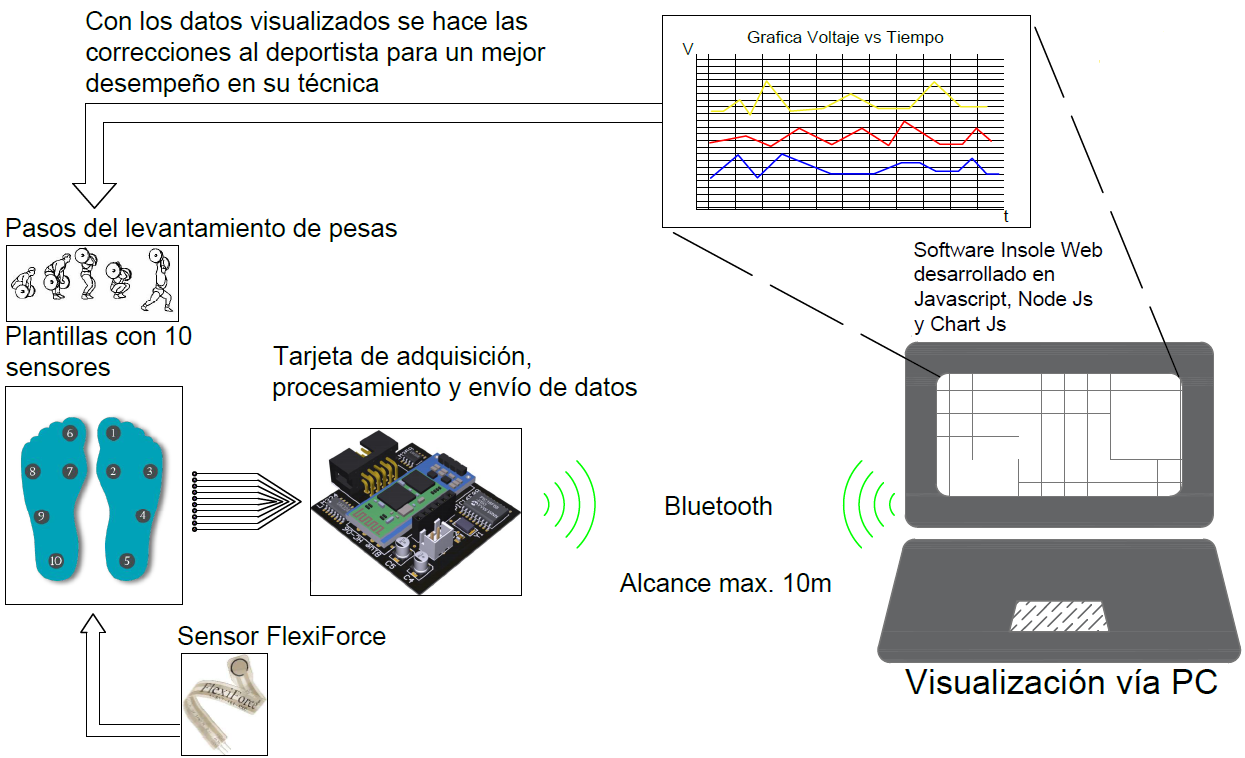
\includegraphics[width=0.83\textwidth]{./image/Diagrama_de_Bloques_sistema_Insole.png}
\caption{Diagrama de Bloques del sistema de adquisición de datos.}
\label{fig:DiagramaBloque}
\end{figure}


\section{Evaluación del Sensor}

\begin{wrapfigure}{r}{0.3\linewidth}
\centering
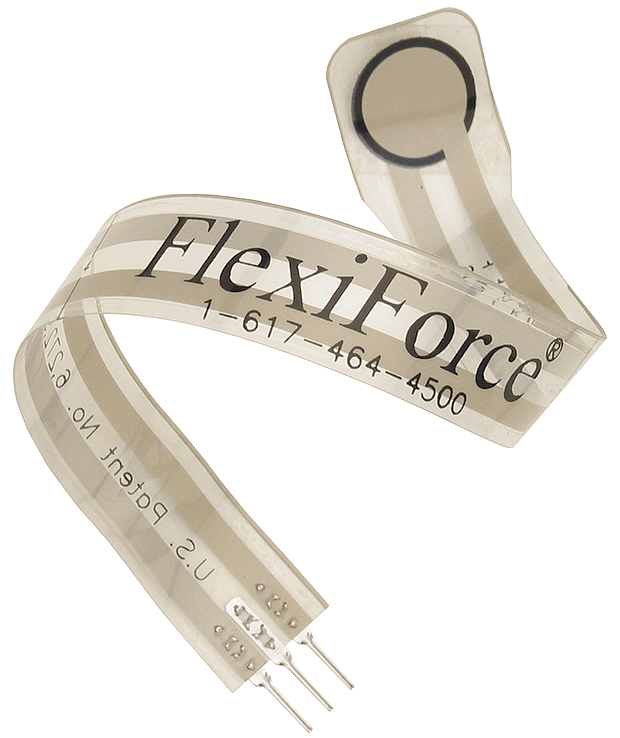
\includegraphics[width=0.2\textwidth]{./image/SensorFlexiForce.png}
\caption{Sensor FlexiForce 100 lbs Tekscan, Piezorresistivo.}
\label{fig:Sensor}
\end{wrapfigure}

El sensor utilizado es el Flexiforce A201, un sensor piezoresistivo delgado y flexible. A mayor fuerza ejercida, la resistencia del sensor se reduce. Las dimensiones del sensor no cambian cuando se flexiona, su rango de fuerza es de $(0-100lbs)$ $440N$, temperatura limite es de $(-9^\circ C$ hasta $60^\circ C)$ y el tiempo de respuesta es de $5$ microsegundos. Con las especificaciones técnicas de los sensores, se diseñaron los circuitos electrónicos para la adquisición de las señales, conversión A/D, y procesamiento.

\begin{figure}[H]
\centering
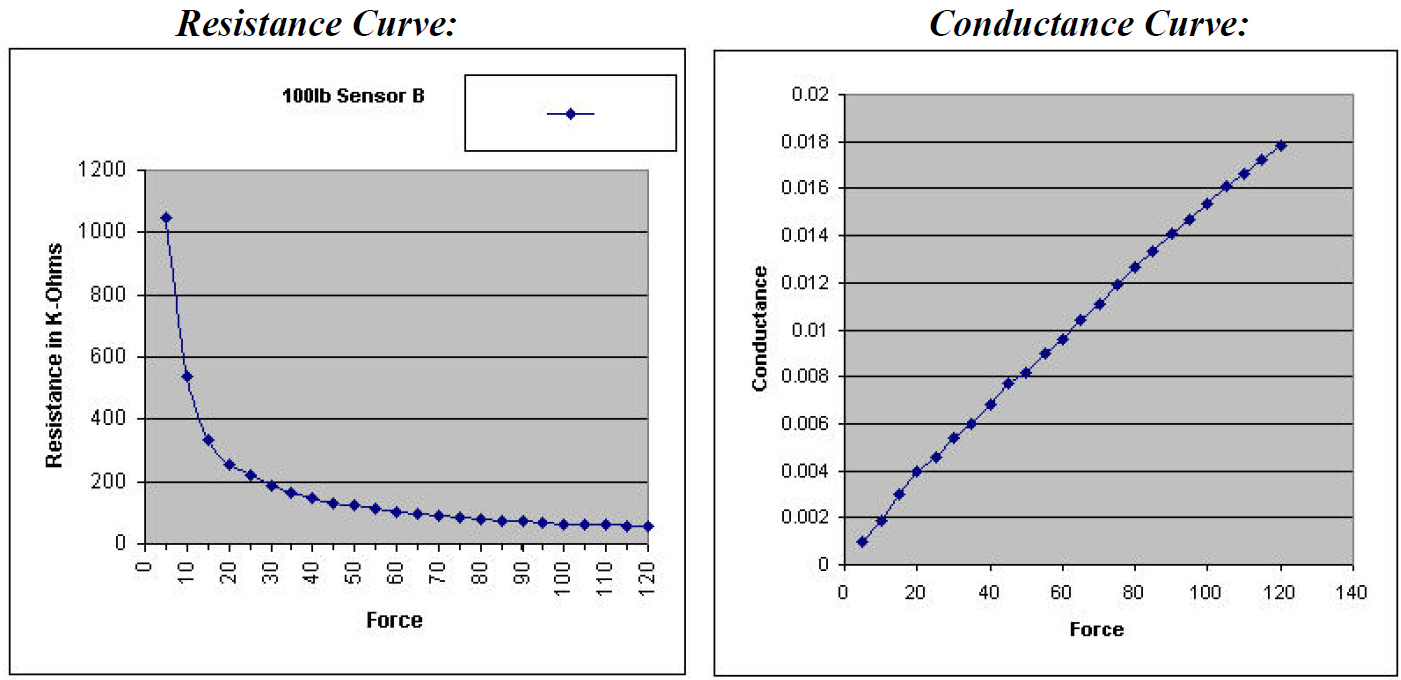
\includegraphics[width=0.9\textwidth]{./image/Curve.png}
\caption{Curvas de Calibración. Fuente: {\href{https://smartxpwiki.ewi.utwente.nl/_media/flx-flexiforce-sensors-manual.pdf}{FlexiForce Sensors Manual.}}}
\label{fig:Curvas}
\end{figure}

\section{Microcontrolador PIC16F88}
Para la selección del microcontrolador se tuvieron en cuenta los siguientes aspectos: el número de pines de entrada analógicos, la opción de empaquetado de montaje superficial y que trabajara con puertos series como son Rx y Tx a 9600 baudios para un correcto funcionamiento con el Bluetooth. Teniendo en cuenta las características anteriormente mencionadas, se eligió el \href{http://ww1.microchip.com/downloads/en/DeviceDoc/30487c.pdf}{PIC16F88} de \href{http://www.microchip.com/}{Microchip} y sus características son presentadas a continuación:

\textbf{Características de baja potencia:}
\begin{itemize}
\item Modos de administración de potencia:
	\begin{itemize}
	\item Primary Run: RC oscillator, 76 $\mu$A, 1MHz, 2V
    \item RC\_RUN: 7 $\mu$A, 31.25kHz, 2V
    \item SEC\_RUN: 9 $\mu$A, 32 kHz, 2V
    \item Sleep: 0.1 $\mu$A, 2V
	\end{itemize}
\item Timer1 Oscillator: 1.8 $\mu$A, 32 kHz, 2V
\item Watchdog Timer: 2.2 $\mu$A, 2V
\item Two-Speed Oscillator Start-up
\end{itemize}

\textbf{Características de los periféricos:}
\begin{itemize}
\item Capture, Compare, PWM (CCP) module:
	\begin{itemize}
	\item Capture is 16-bit, max. resolution is 12.5 ns
    \item Compare is 16-bit, max. resolution is 200 ns
    \item PWM max. resolution is 10-bit
	\end{itemize}
\item 10-bit, 7-channel Analog-to-Digital Converter
\item Synchronous Serial Port (SSP) with SPI™ (Master/Slave) and I$^{2}$C™ (Slave)
\item Addressable Universal Synchronous Asynchronous Receiver Transmitter (AUSART/SCI) with 9-bit address detection:
	\begin{itemize}
	\item RS-232 operation using internal oscillator (no external crystal required)
	\end{itemize}
\item Dual Analog Comparator module:
	\begin{itemize}
	\item Programmable on-chip voltage reference
    \item Programmable input multiplexing from device inputs and internal voltage reference
    \item Comparator outputs are externally accessible
	\end{itemize}
\end{itemize}

\textbf{Características especiales del Microcontrolador:}
\begin{itemize}
\item 100.000 erase/write cycles Enhanced Flash program memory typical
\item 1.000.000 typical erase/write cycles EEPROM data memory typical
\item EEPROM Data Retention: > 40 years
\item In-Circuit Serial Programming™ (ICSP™) via two pins
\item Processor read/write access to program memory
\item Low-Voltage Programming
\item In-Circuit Debugging via two pins
\item Extended Watchdog Timer (WDT):
	\begin{itemize}
	\item Programmable period from 1 ms to 268s
	\end{itemize}
\item Wide operating voltage range: 2.0V to 5.5V
\end{itemize}

\begin{figure}[H]
\centering
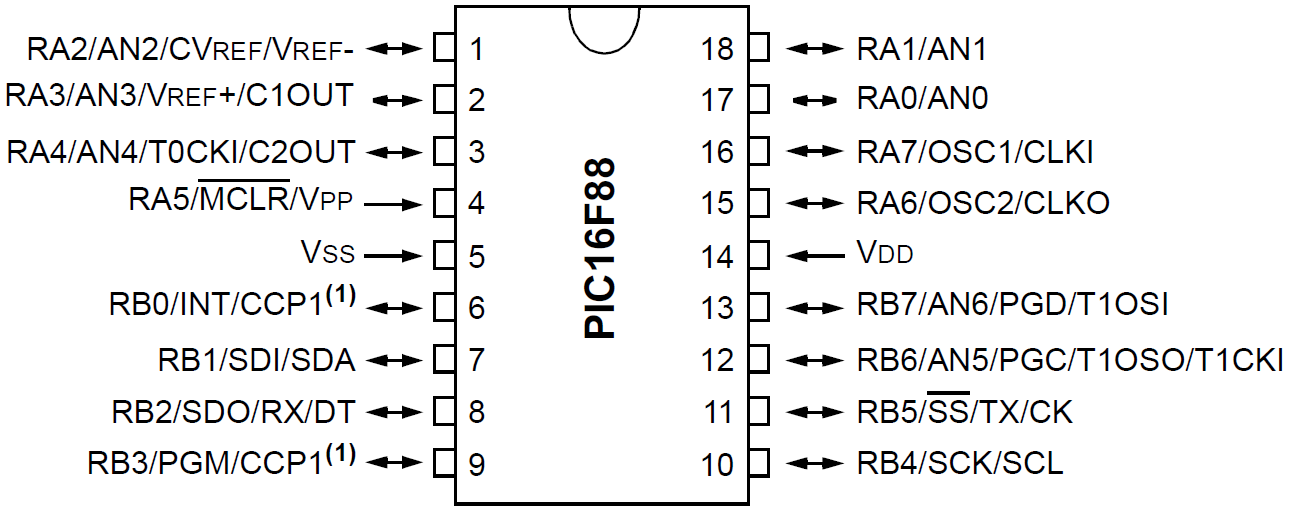
\includegraphics[width=0.9\textwidth]{./image/PIC16F88.png}
\caption{Diagrama de pines PIC16F88.}
\label{fig:PIC16F88}
\end{figure}


\section{Modulo Bluetooth HC-06}

Se seleccionó la tecnología Bluetooth por su bajo consumo de potencia, alcance y bajo costo. Las características del modulo HC-06 son:
\begin{itemize}
\item Led indicadores de conexión y encendido.
\item Alcance: 10m aproximados.
\item Compatible con el protocolo Bluetooth V2.0.
\item Voltaje de alimentación: 3.3VDC $\sim$ 6VDC.
\item Voltaje de operación: 3.3VDC.
\item Corriente: < 40 mA
\item Velocidad de comunicación ajustable: 1200, 2400, 4800, 9600, 19200, 38400, 57600, 115200 baud.
\item Medidas: 1.73 in x 0.63 in x 0.28 in (4.4 cm x 1.6 cm x 0.7 cm)
\item Número de pines: 4
\end{itemize}

\begin{figure}[H]
\centering
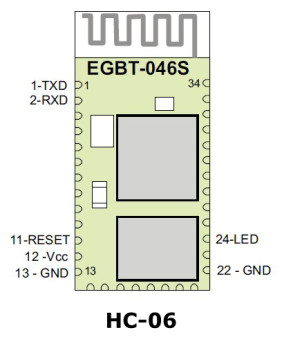
\includegraphics[width=0.3\textwidth]{./image/Blue_HC-06.png}
\caption{Modulo Bluetooth HC-06.}
\label{fig:Blue_HC-06}
\end{figure}

Su reducido tamaño permite cumplir con uno de los objetivos principales de portabilidad del sistema el cual no interviene en la practica del deporte a monitorear. 

\section{Diseño y fabricación del circuito impreso para la adquisición y envío de datos}

Para el diseño del circuito se tienen en cuenta las diferentes etapas que son la alimentación de la tarjeta, la adquisición de datos, el procesamiento de datos y la comunicación para el envío de datos.

\begin{figure}[H]
 \centering
  \subfloat[Software Altium Design versión 18.]{
   \label{fig:AltiumDesign}
    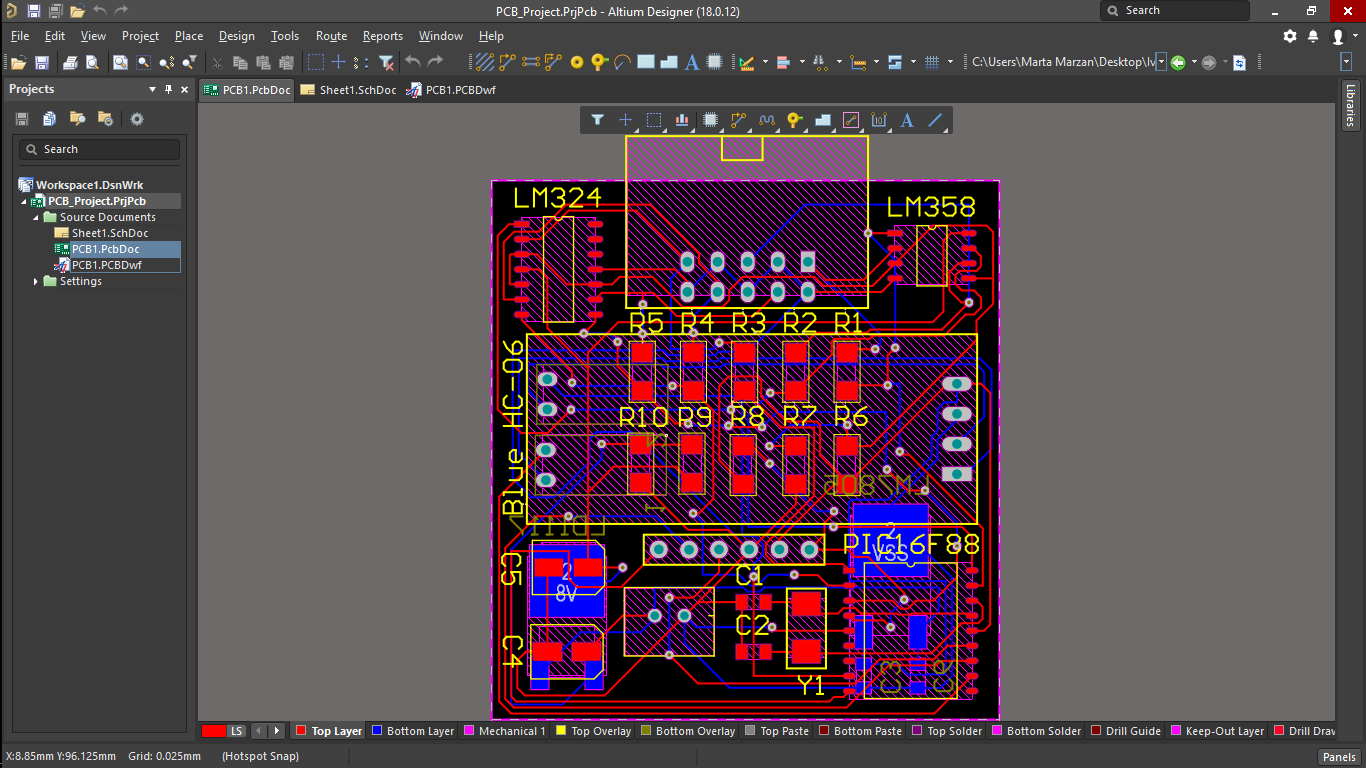
\includegraphics[width=0.49\textwidth]{./image/AltiumDesign.png}}
    \subfloat[Software SolidWorks versión 17.]{
   \label{fig:SolidWorks}
    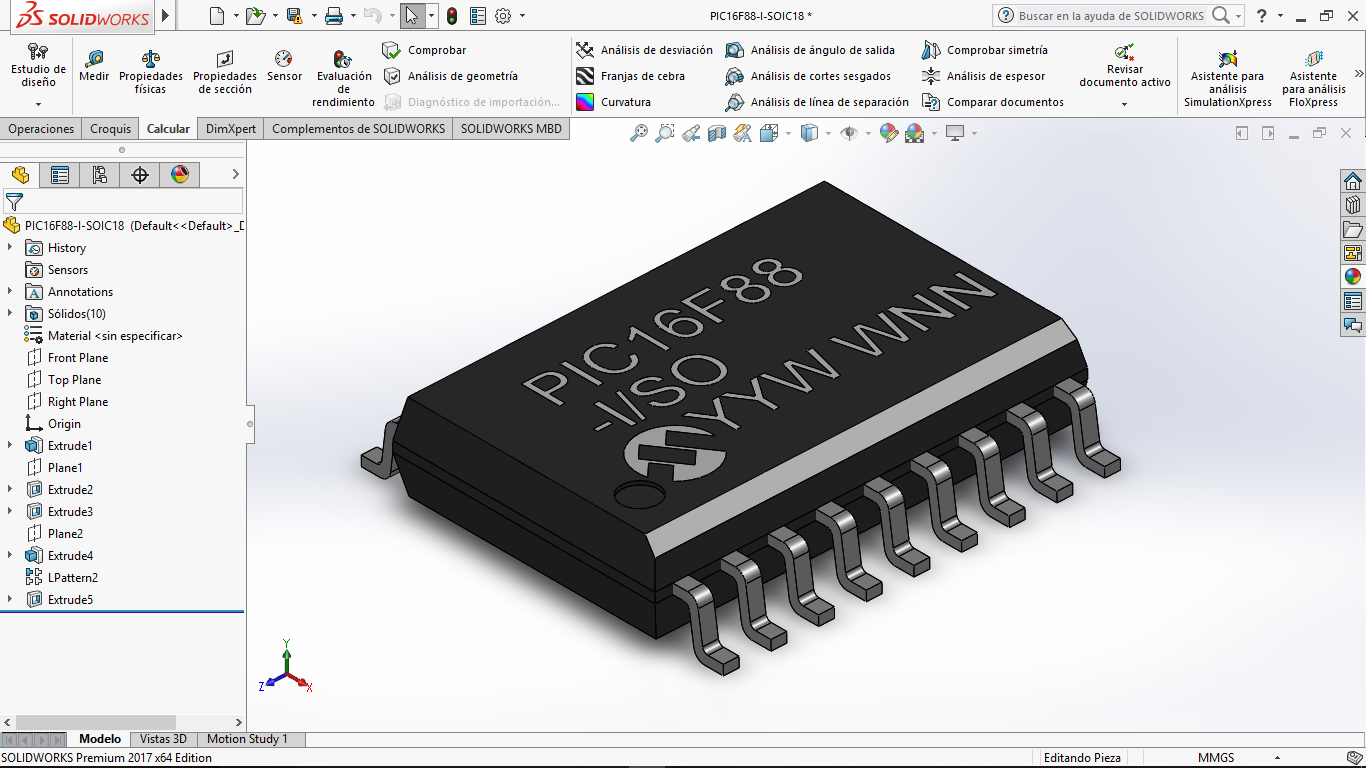
\includegraphics[width=0.49\textwidth]{./image/Solid_PIC16F88_3D.png}}\\
    \subfloat[Software Proteus versión 8.5.]{
   \label{fig:Proteus}
    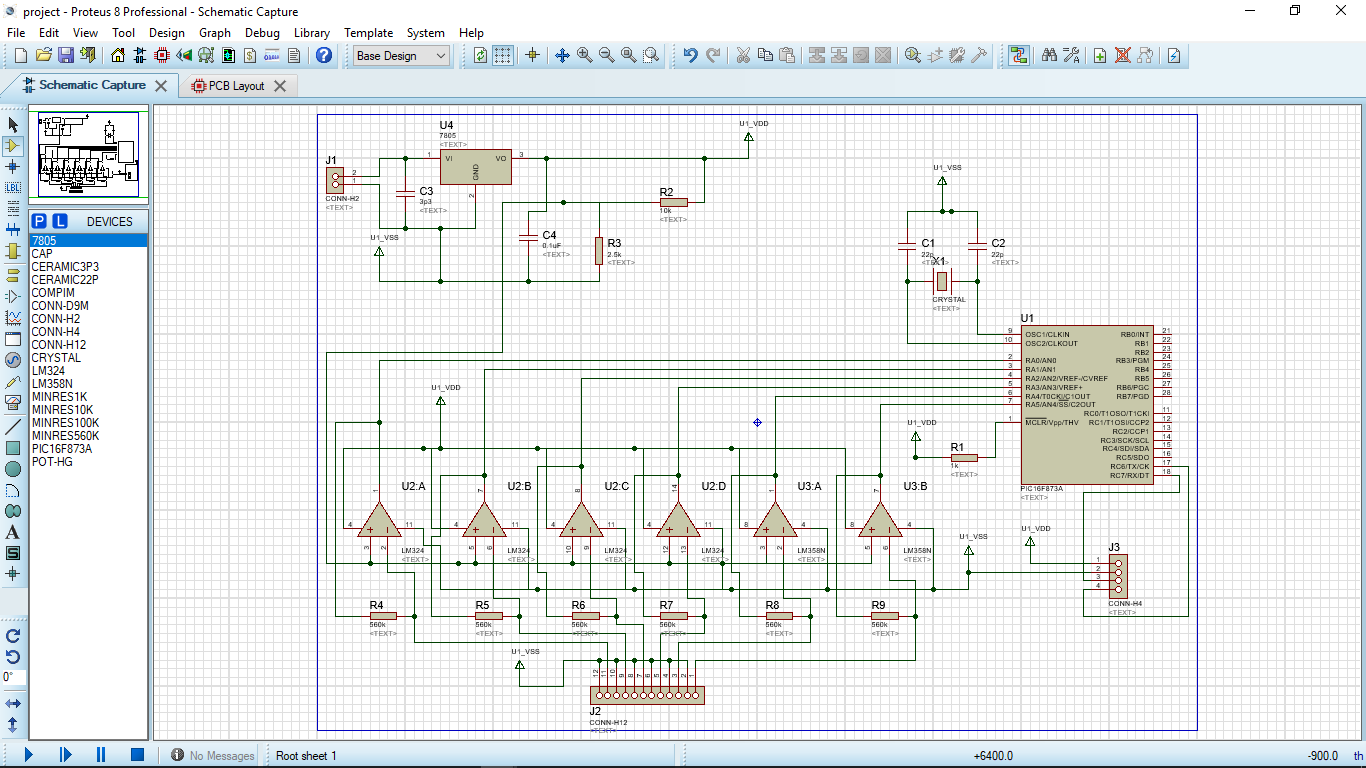
\includegraphics[width=0.49\textwidth]{./image/Proteus_esquematico.png}}
    \subfloat[Software miKroC for PIC versión 17.]{
   \label{fig:mickroC}
    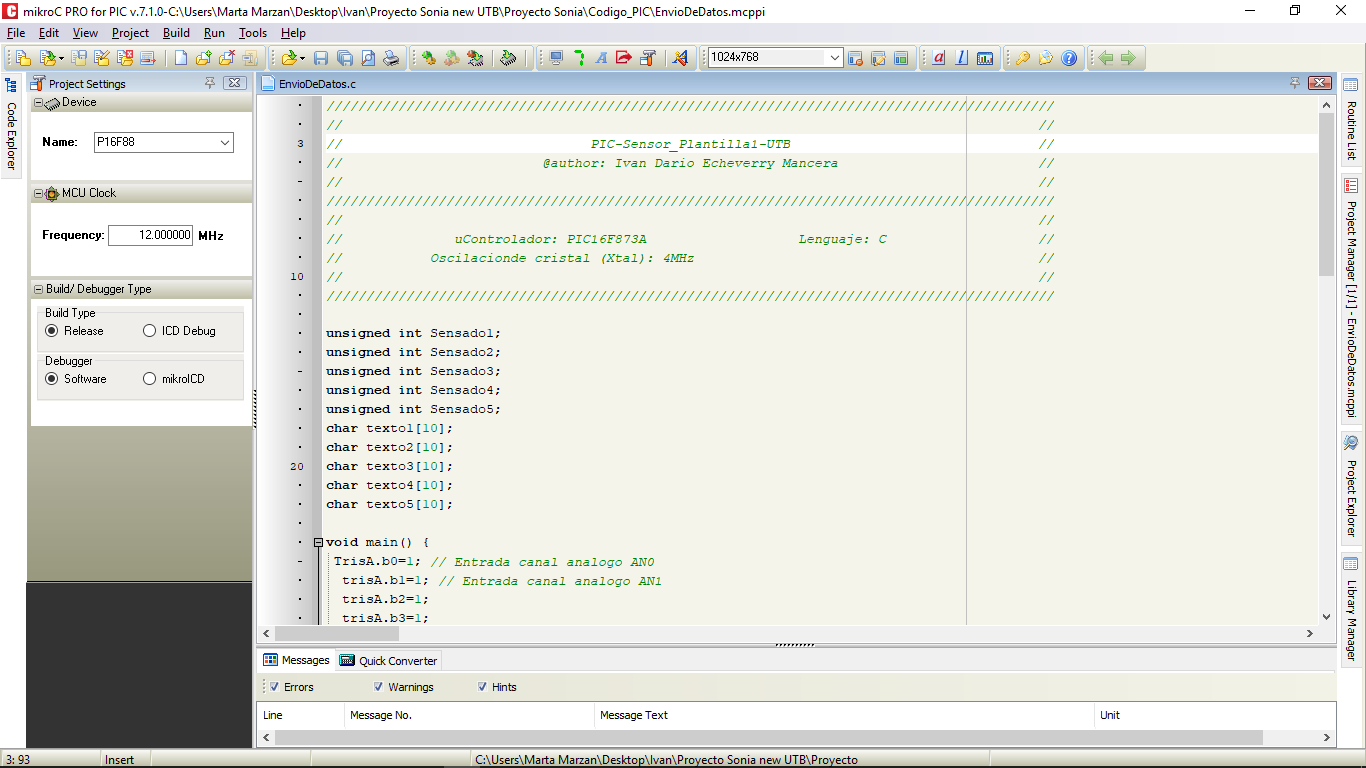
\includegraphics[width=0.49\textwidth]{./image/microC_for_PIC.png}}
 \caption{Tipos de Software utilizados para el diseño del sistema.}
 \label{fig:Software}
\end{figure}

Los programas computacionales utilizados para la simulación, diseño y elaboración de la tarjeta PCB son \href{https://www.labcenter.com/}{Proteus} versión 8.5 de Labcenter y \href{https://www.altium.com/altium-designer/es}{Altium Design} versión 18. Además se utilizó el software de diseño CAD \href{http://www.solidworks.es/}{SolidWorks} versión 17 para el diseño 3D de los componentes del circuito. Este programa se complementa con \href{https://www.altium.com/altium-designer/es}{Altium Design}. Para obtener mejores resultados se utilizaron librerías o modelos ya creados por otros usuarios de SolidWorks que se encuentran alojados en 3DContentCentral (\href{http://www.3dcontentcentral.es/}{http://www.3dcontentcentral.es/}) de forma libre para su desarrollo.

A continuación se describirá el circuito, que consta de las siguientes etapas: etapa (1) de alimentación, etapa (2) de adquisición y acondicionamiento de los datos y etapa (3) de procesamiento y transmisión de datos.

\begin{figure}[H]
\centering
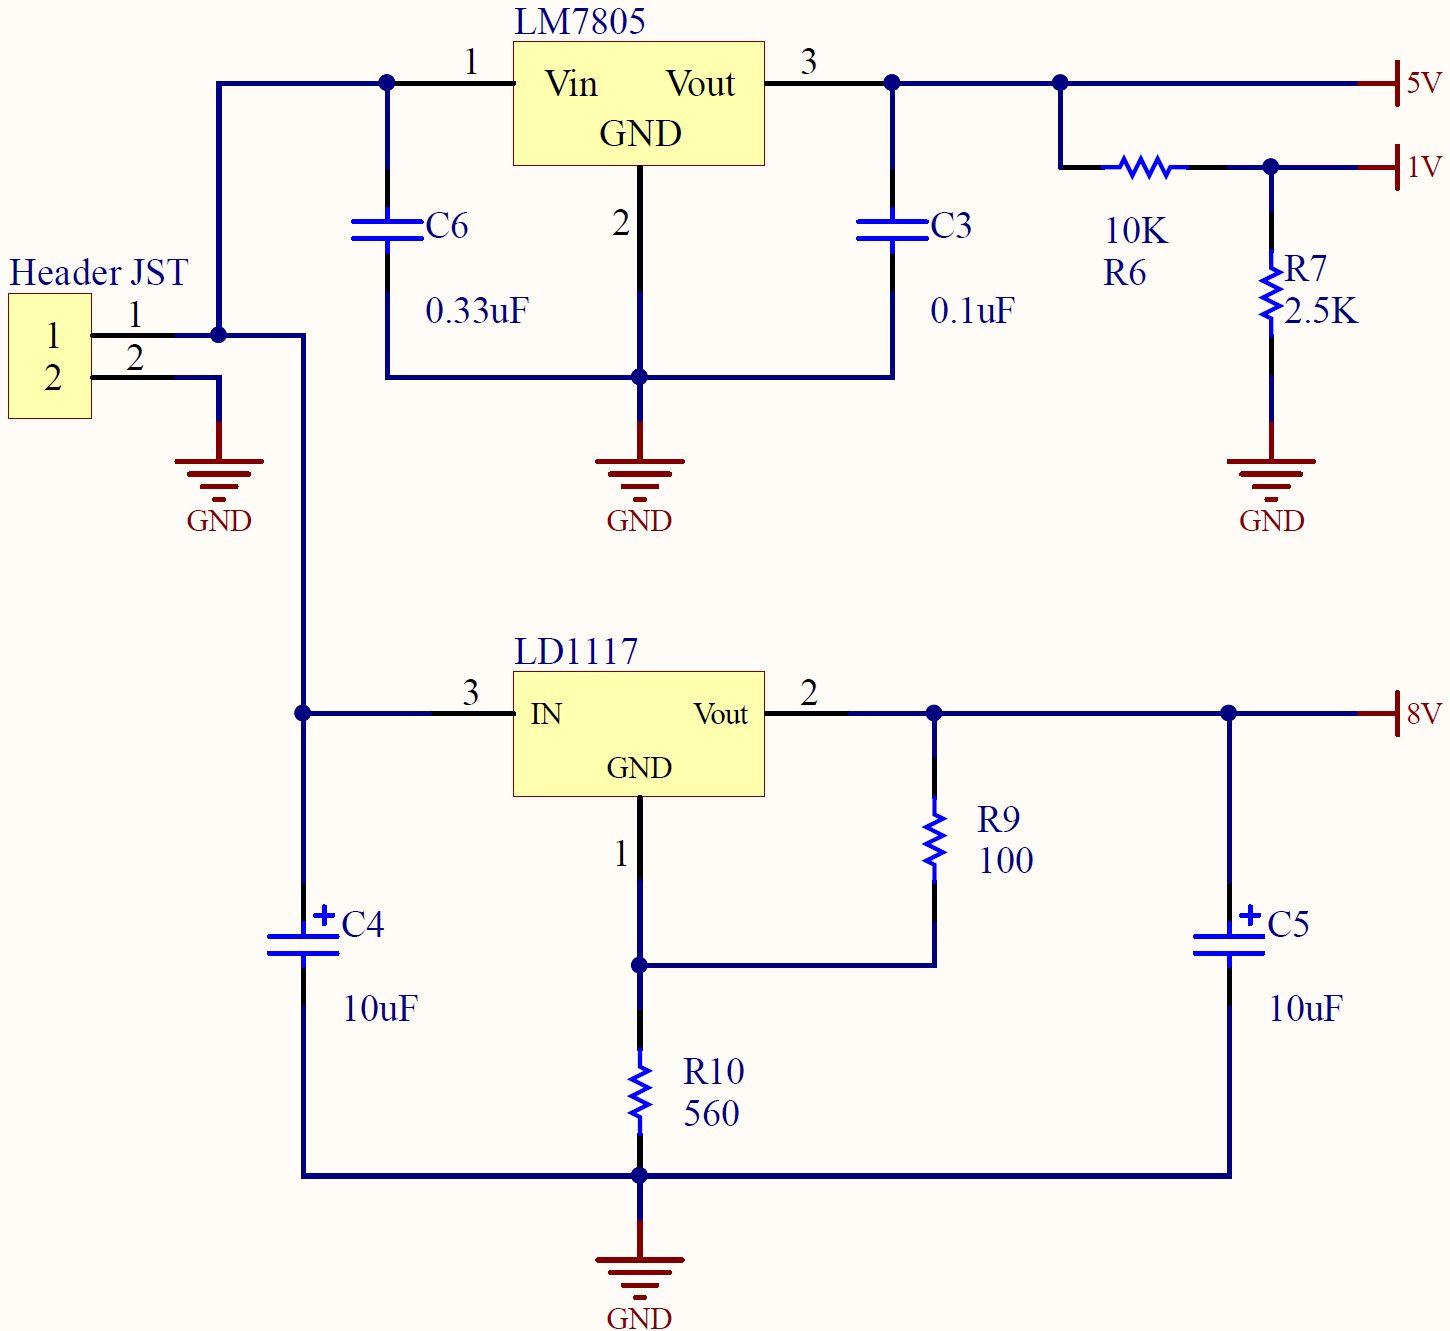
\includegraphics[width=0.6\textwidth]{./image/CircuitoFuente.png}
\caption{Etapa 1, Fuentes de 5V, 8V y Referencia de 1V.}
\label{fig:EtapaFuente}
\end{figure}

En la etapa (1) de alimentación de la tarjeta se usaron dos reguladores de voltaje para asegurar dos fuentes una de 5 Voltios y otra de 8 Voltios, y un voltaje de referencia como señal para la entrada al amplificador operacional de 1 Voltio. Para la fuente de 5 Voltios se utilizó un integrado de montaje superficial \href{https://www.sparkfun.com/datasheets/Components/LM7805.pdf}{LM7805}, este es utilizado para alimentar el microcontrolador \href{http://ww1.microchip.com/downloads/en/DeviceDoc/30487c.pdf}{PIC16F88}, el modulo \href{https://www.olimex.com/Products/Components/RF/BLUETOOTH-SERIAL-HC-06/resources/hc06.pdf}{Bluetooth HC-06}, darle Reset a la Tarjeta y derivar 1 Voltio para la referencia de los amplificadores operacionales por medio de un divisor de tensión. La regulación de 8 Voltios lograda con un integrado \href{https://cdn-shop.adafruit.com/product-files/2165/LD1117.pdf}{LD1117} es utilizada para la alimentación de dos amplificadores operacionales (\href{http://www.ti.com/lit/ds/symlink/lm158-n.pdf}{LM358} y \href{http://www.ti.com/lit/ds/symlink/lm124-n.pdf}{LM324}) cumpliendo así que este valor sea 2 Voltios mayor al máximo valor obtenido en la salida (OUT) de los amplificadores. El integrado \href{https://cdn-shop.adafruit.com/product-files/2165/LD1117.pdf}{LD1117} es un regulador variable y su ajuste viene definido por la siguiente ecuación:
\begin{center}
${{V}_{OUT}}={{V}_{REF}}(1+{{R}_{2}}/{{R}_{1}})$
\end{center}
Con base en el circuito que recomienda el fabricante (figura \ref{fig:circuitoejemplo}) y su ecuación podemos calcular el voltaje de salida de la siguiente manera:
\begin{figure}[H]
\centering
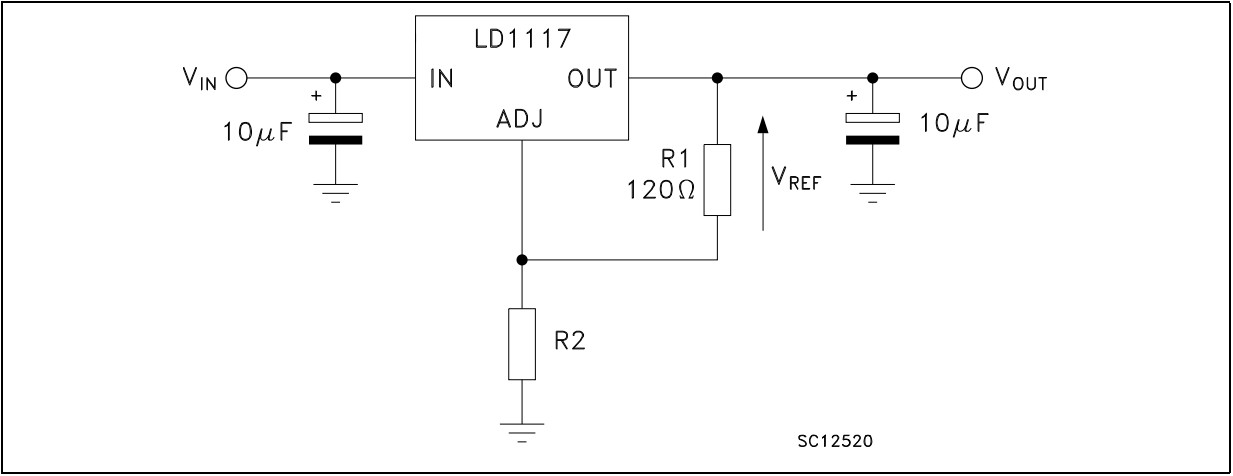
\includegraphics[width=0.9\textwidth]{./image/circuitoejemplo.png}
\caption{Aplicación de salida con voltaje ajustable. Fuente: \href{https://cdn-shop.adafruit.com/product-files/2165/LD1117.pdf}{LD1117}.}
\label{fig:circuitoejemplo}
\end{figure}
Dándole valores constantes a ${V}_{REF}=1.25V$, ${V}_{OUT}=8V$ y ${R}_{1}=100\Omega$ procedemos a despejar ${R}_{2}$:
\begin{center}
${R}_{2}=(({V}_{OUT}/{V}_{REF})-1)\times{R}_{1}$\\
${R}_{2}=((8V/1.25V)-1)\times100\Omega$\\
${R}_{2}=540\Omega$
\end{center}

\begin{figure}[H]
\centering
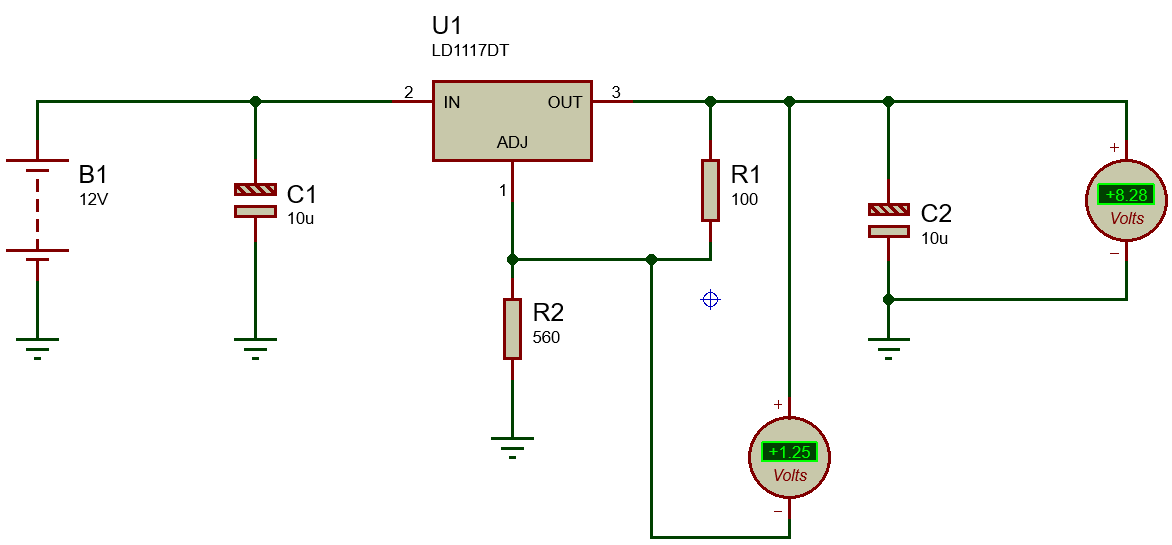
\includegraphics[width=0.9\textwidth]{./image/Simulacion_LD1117.png}
\caption{Simualción del circuito para el voltaje ajustable a 8V.}
\label{fig:SimulacionLD1117}
\end{figure}

Como buena practica se realizó la simulación en el software Proteus, el cual arrojó el resultado observado en la figura \ref{fig:SimulacionLD1117}.

En la etapa (2) (figura \ref{fig:EtapaAdquisicion}) encontramos la parte de adquisición, acondicionamiento y entrega de datos al microcontrolador, esta etapa esta compuesta por dos amplificadores operacionales un \href{http://www.ti.com/lit/ds/symlink/lm158-n.pdf}{LM358} el cual contiene dos amplificadores usados para los sensores 1 y 2 de la plantilla y un \href{http://www.ti.com/lit/ds/symlink/lm124-n.pdf}{LM324} que tiene los cuatro amplificadores usados para los sensores 3, 4 y 5. Estos amplificadores operacionales cumplen la función de proteger el circuito del microcontrolador de impedancias altas en las entradas del mismo.

\begin{figure}[H]
\centering
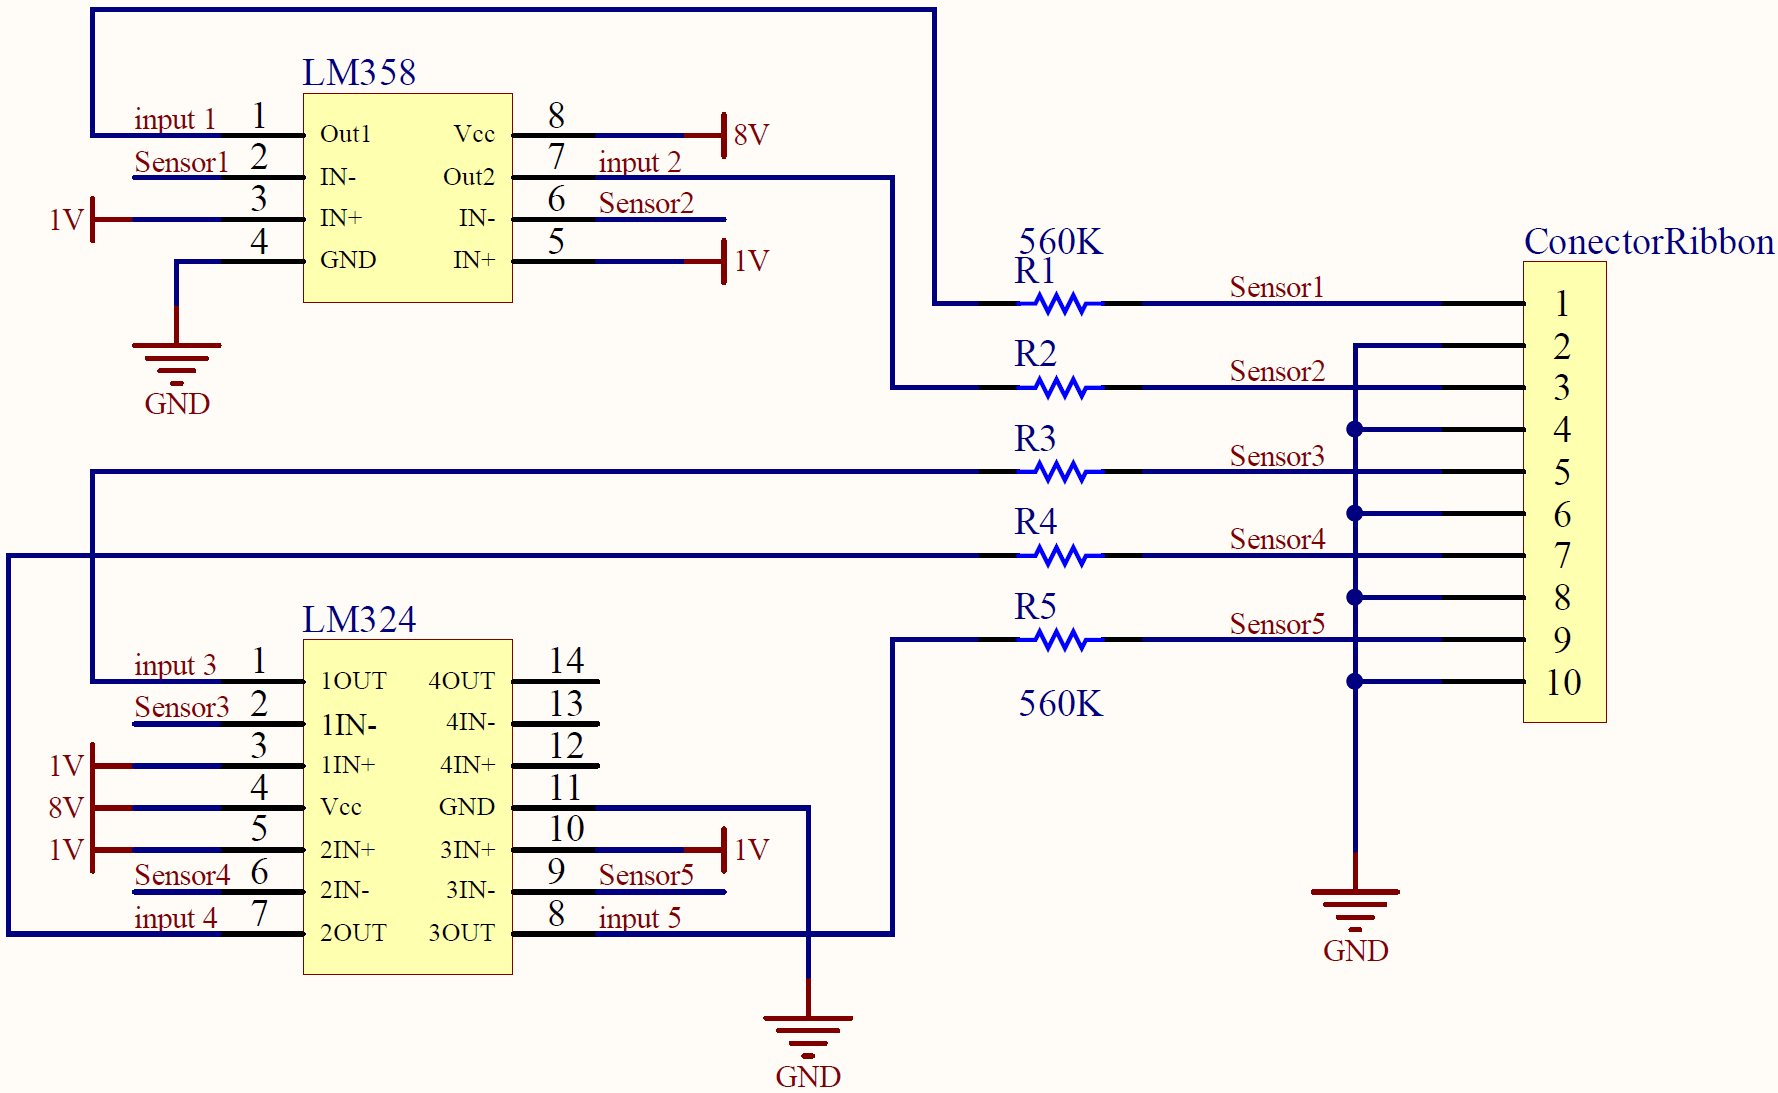
\includegraphics[width=0.7\textwidth]{./image/EtapaAdquisicionDatos.png}
\caption{Etapa 2, Etapa de Amplificadores Operacionales para la adquisición y acondicionamiento de los datos reflejados de cada Sensor.}
\label{fig:EtapaAdquisicion}
\end{figure}

\begin{figure}[H]
\centering
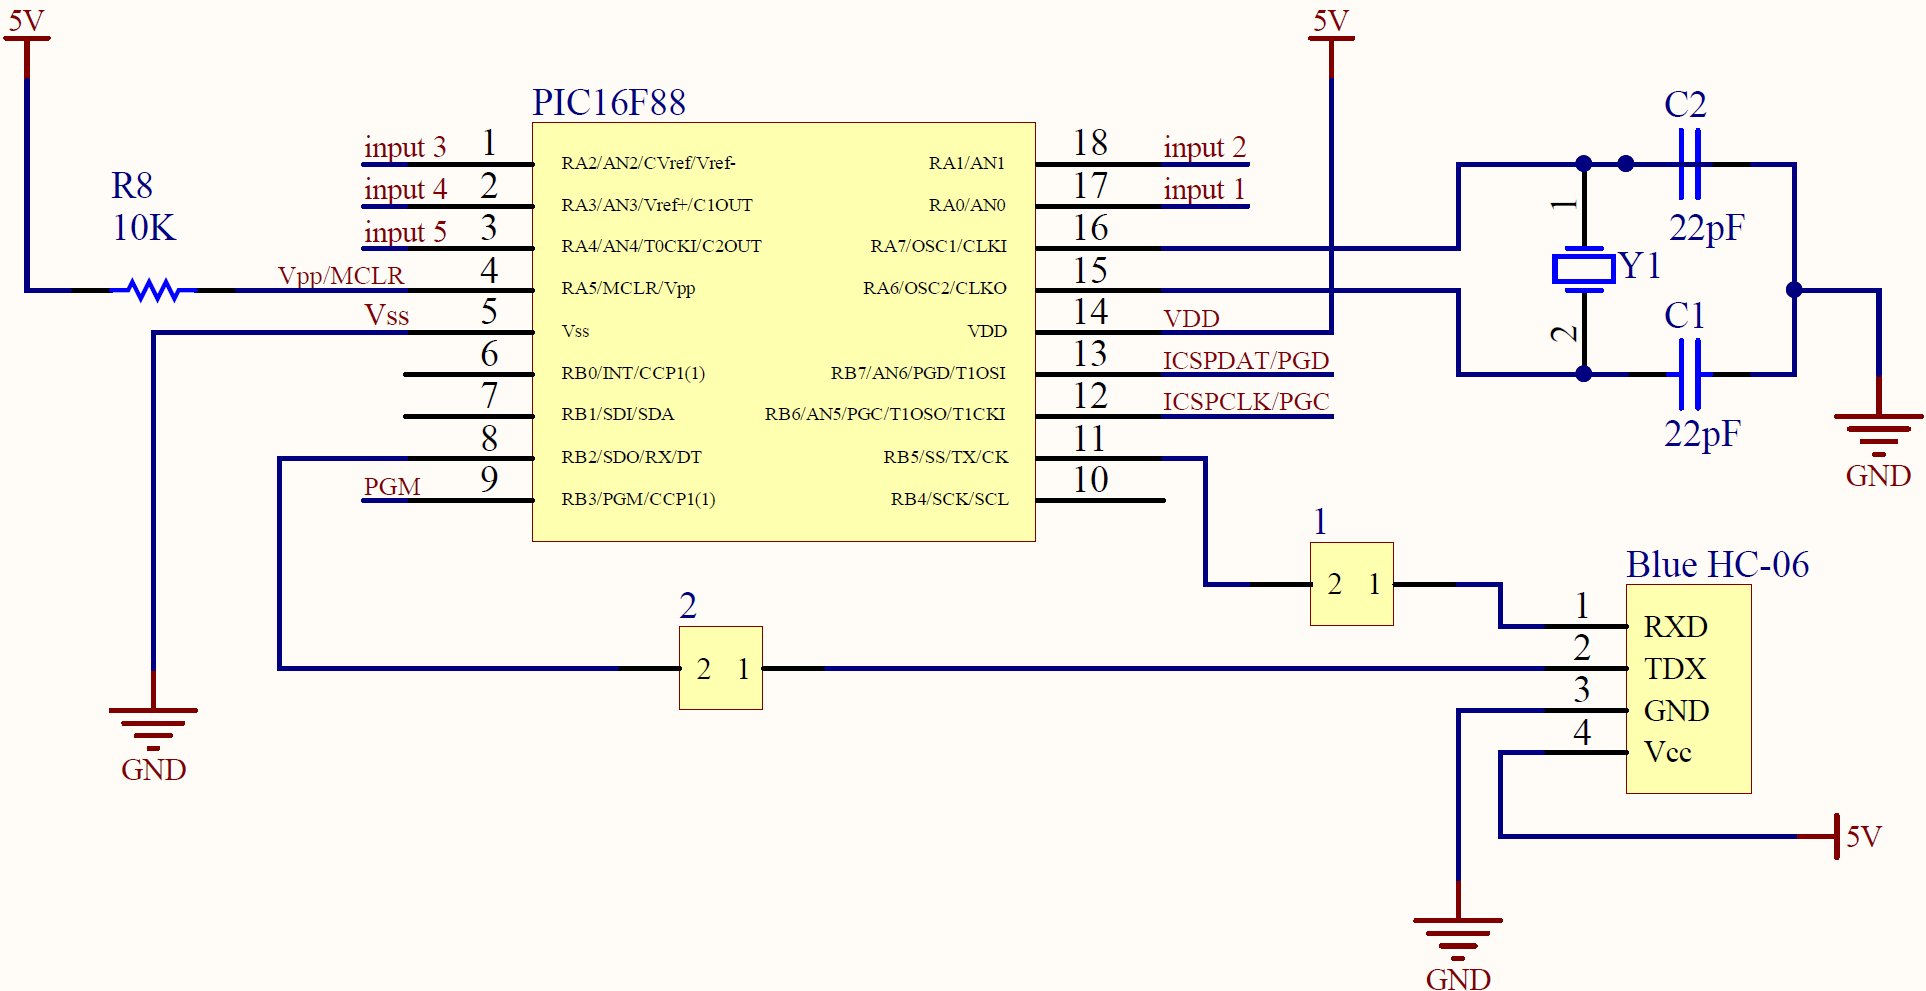
\includegraphics[width=0.7\textwidth]{./image/CircuitouControl.png}
\caption{Etapa 3, Etapa de procesamiento y envío mediante Bluetooth de los datos.}
\label{fig:EtapaProcesamiento}
\end{figure}

La etapa (3) esta compuesta por un microcontrolador de montaje superficial \href{http://ww1.microchip.com/downloads/en/DeviceDoc/30487c.pdf}{PIC16F88} el cual recibe los datos de los amplificadores operacionales y los procesa para posteriormente enviarlos por el puerto serie hacia el Bluetooth HC-06 y este último se encarga de hacer enlace con el computador con su antena a 2.4GHz.

\begin{figure}[H]
\centering
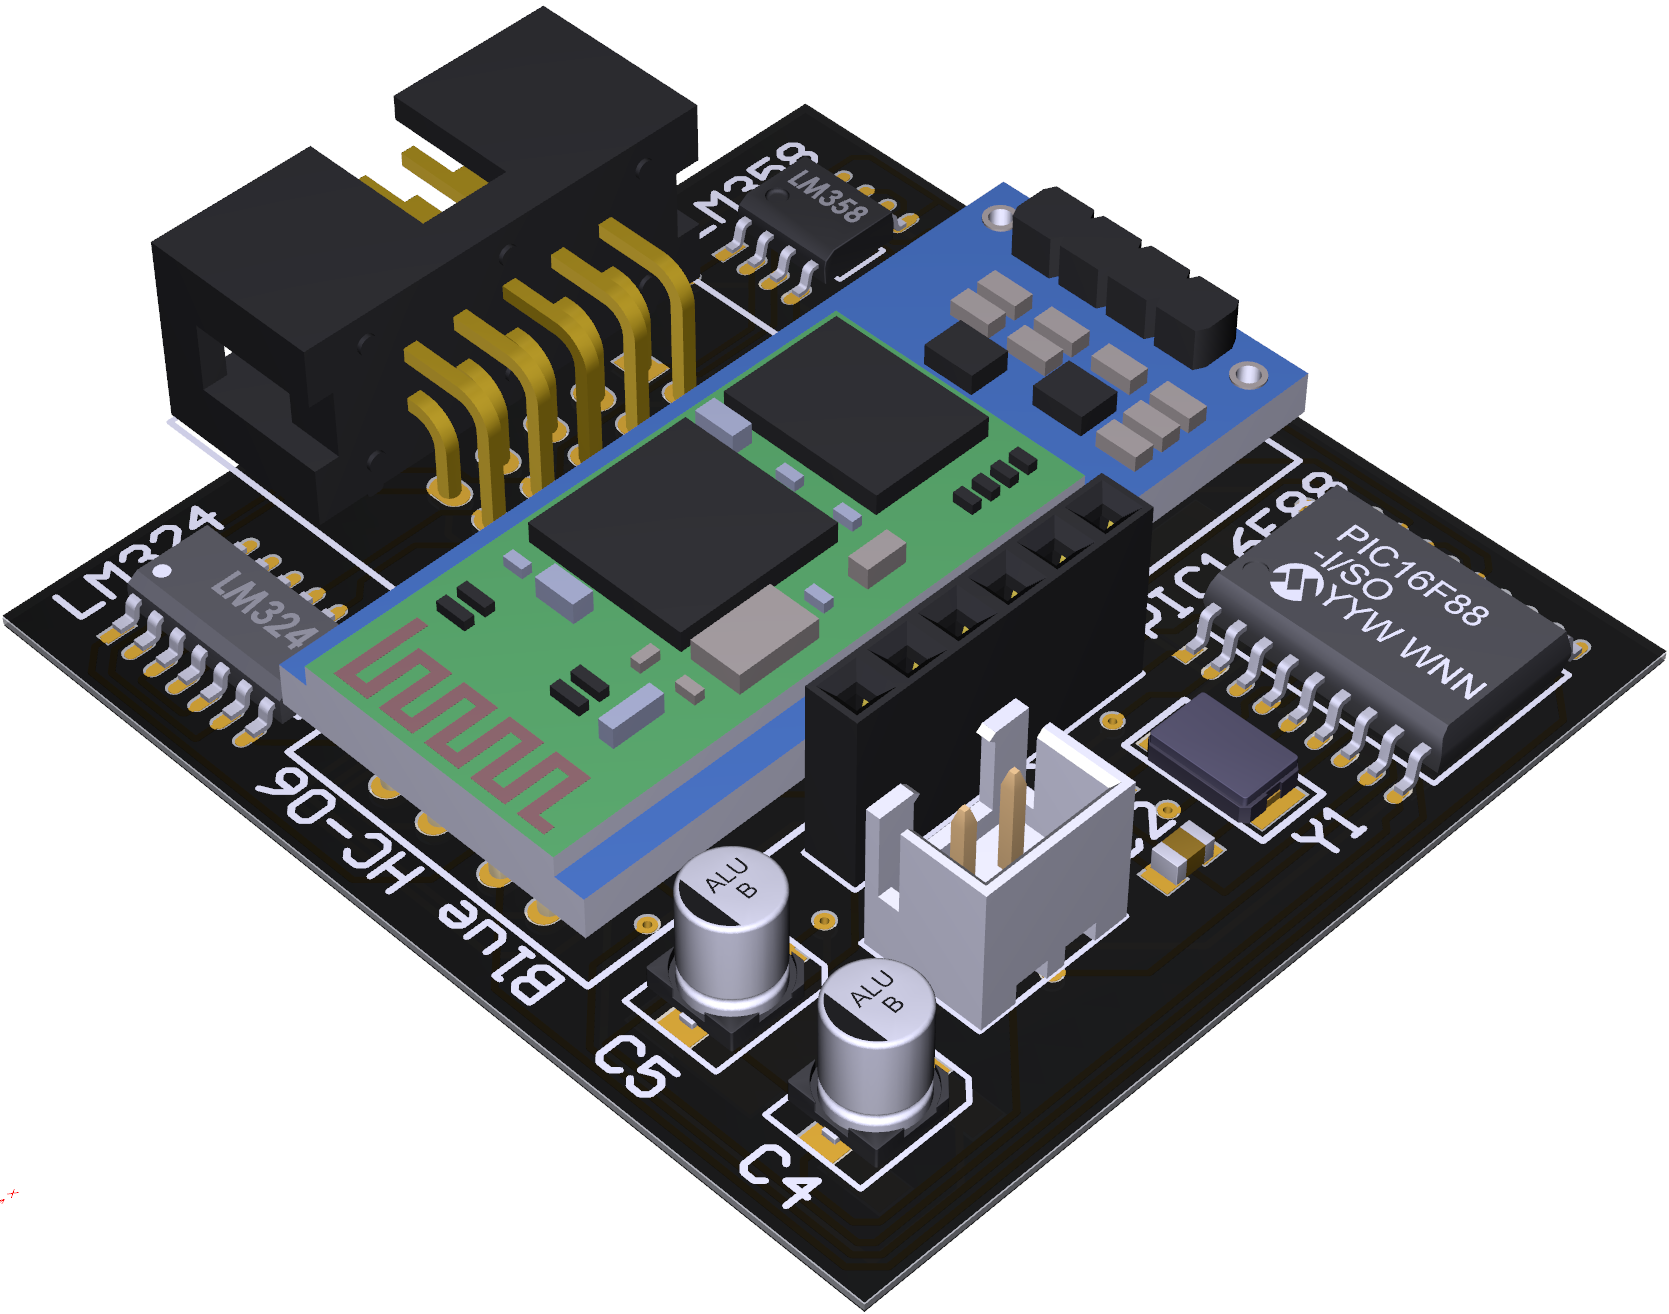
\includegraphics[width=0.7\textwidth]{./image/CircuitoSMD.png}
\caption{Tarjeta 3D de Adquisición, Procesamiento y envío de Datos.}
\label{fig:CircuitoSMD}
\end{figure}

\section{Calibración de Sensores}

En esta etapa se efectuaron pruebas de fuerza con 5 sensores de igual capacidad. Se realizaron pruebas con distintos valores de fuerza en los sensores y se obtuvieron mediciones similares entre sí, con lo cual se verificó que la calibración fue correcta. En la Fig. \ref{fig:Comportamiento} se puede observar los diferentes comportamientos para cada sensor de forma individual y con mas detalle se pueden ver estos valores en la Tabla \ref{Table:Valores}. Resulta importante aclarar que cada sensor arrojó valores que difieren un poco pero siguen un mismo patrón de forma lineal siendo su resistencia inversamente proporcional a la presión ejercida en cada sensor.

\begin{table}[H]
%\small
%\footnotesize
\scriptsize
%\tiny
\begin{center}
\begin{tabular}{| c | c | c | c | c | c |}
 \hline
\textbf{Sensor} & \textbf{Medida} & \textbf{Fuerza [KN]} & \textbf{Voltaje [V]} & \textbf{Voltaje min.} & \textbf{Voltaje max.} \\ 
 \hline
                    & 1 & 0,059 & 1,99 & 1,93 & 2,05 \\  
                    & 2 & 0,12 & 2,05 & 1,97 & 2,12 \\
                    & 3 & 0,168 & 2,33 & 2,28 & 2,37 \\
    1               & 4 & 0,205 & 2,62 & 2,57 & 2,68 \\
                    & 5 & 0,31 & 2,76 & 2,72 & 2,80 \\
                    & 6 & 0,432 & 3,75 & 3,73 & 3,77 \\
 \hline
                    & 7 & 0,06 & 2,10 & 2,04 & 2,16 \\
 					& 8 & 0,13 & 2,34 & 2,28 & 2,40 \\
    2               & 9 & 0,2 & 2,66 & 2,61 & 2,71 \\  
 					& 10 & 0,32 & 2,86 & 2,82 & 2,89 \\
 					& 11 & 0,42 & 3,02 & 2,99 & 3,06 \\
 \hline
					& 12 & 0,055 & 2,02 & 1,94 & 2,11 \\
					& 13 & 0,0115 & 2,11 & 2,05 & 2,18 \\
    3				& 14 & 0,21 & 2,39 & 2,34 & 2,45 \\
					& 15 & 0,3 & 2,55 & 2,45 & 2,65 \\
					& 16 & 0,43 & 2,86 & 2,82 & 2,91 \\
 \hline
					& 17 & 0,06 & 2,12 & 2,06 & 2,19 \\  
 					& 18 & 0,139 & 2,54 & 2,49 & 2,58 \\
	4				& 19 & 0,2 & 2,94 & 2,89 & 2,99 \\
					& 20 & 0,33 & 3,36 & 3,32 & 3,39 \\
					& 21 & 0,43 & 3,87 & 3,82 & 3,92 \\
 \hline
					& 22 & 0,055 & 1,96 & 1,83 & 2,08 \\
					& 23 & 0,13 & 2,05 & 1,93 & 2,17 \\
	5				& 24 & 0,215 & 2,34 & 2,29 & 2,38 \\
					& 25 & 0,315 & 2,61 & 2,58 & 2,64 \\
					& 26 & 0,435 & 3,41 & 3,36 & 3,45 \\
 \hline
\end{tabular}
\caption{Valores obtenidos en la caracterización de cada sensor.}
\label{Table:Valores}
\end{center}
\end{table}

\begin{figure}[H]
\centering
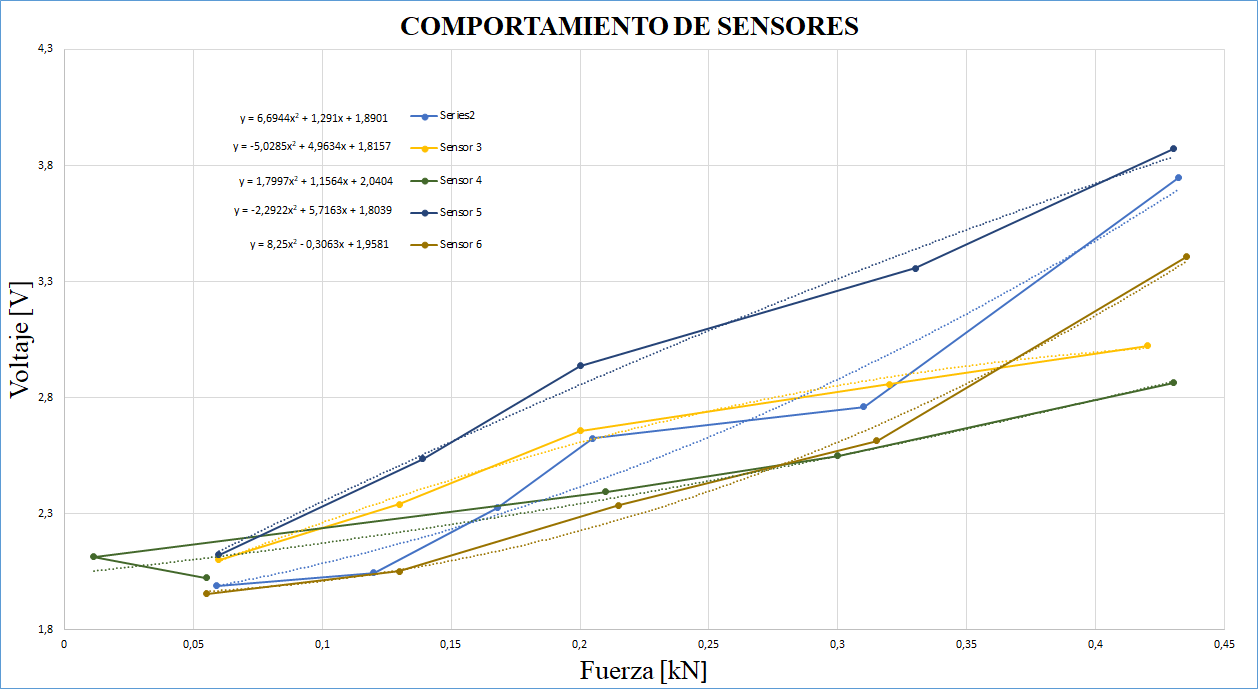
\includegraphics[width=1\textwidth]{./image/ComportamientoSensores.png}
\caption{Gráfica obtenida de la calibración de sensores.}
\label{fig:Comportamiento}
\end{figure}

\begin{figure}[H]
\centering
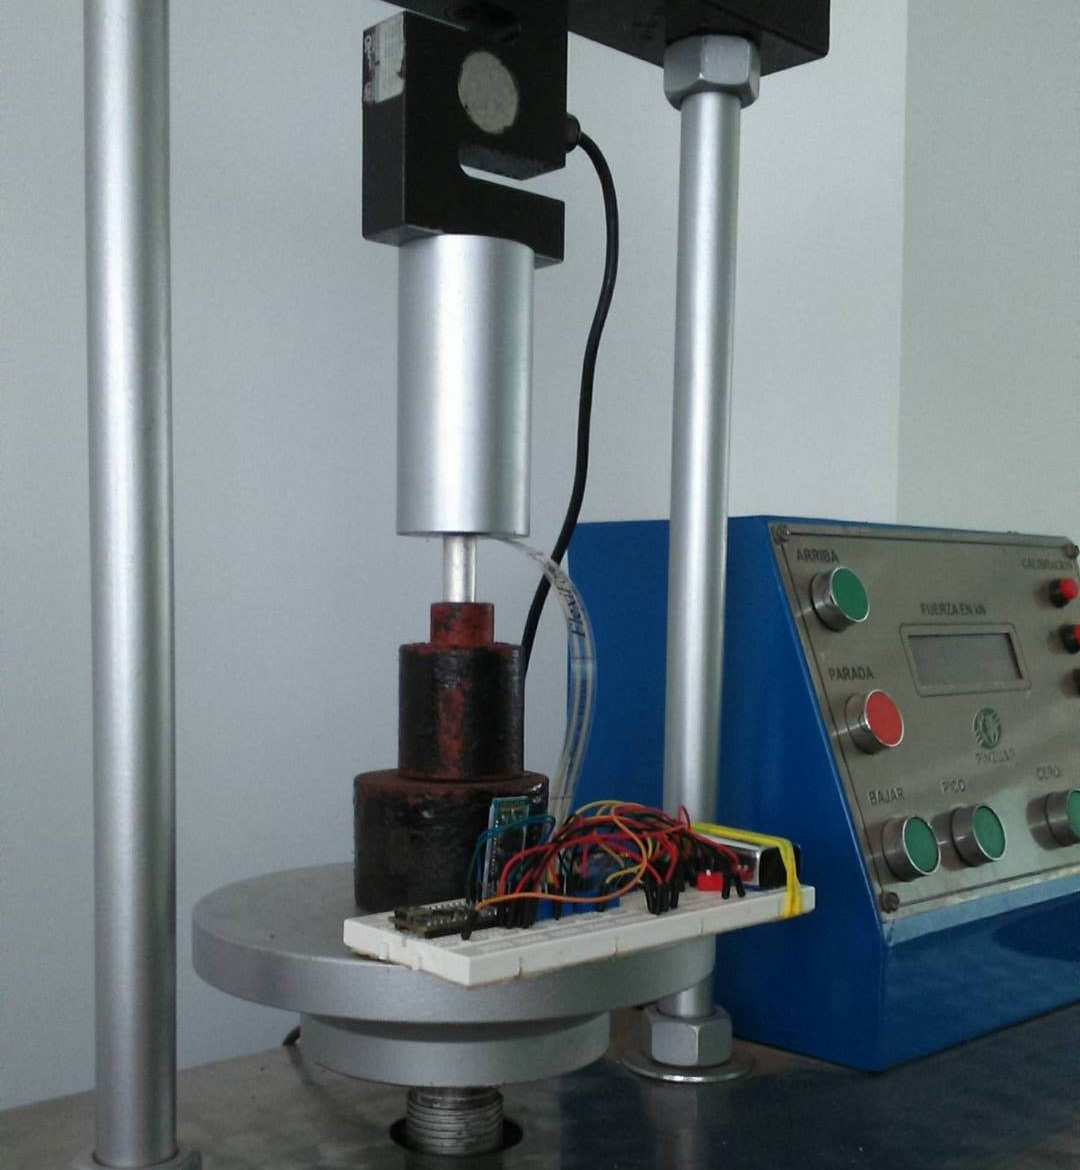
\includegraphics[width=0.5\textwidth]{./image/2.jpg}
\caption{Montaje para la calibración de sensores.}
\label{fig:Montaje}
\end{figure}

Para la calibración de estos sensores el montaje utilizado se puede visualizar en la Fig. \ref{fig:Montaje} donde se utilizó la maquina semiautomática digital para ensayos Marshall y CBR del laboratorio de suelos de la Universidad Tecnológica de Bolívar.

La Máquina Digital para Ensayos Marshall y CBR PS-25 esta diseñada para la exactitud, rapidez y registro confiable de los resultados adquiridos. Cuenta con un mecanismo de operación manual por medio de manivela para los ensayos de CBR (California Bearing Ratio: Ensayo de Relación de Soporte de California) mide la resistencia al esfuerzo cortante de un suelo en cemento, y operación eléctrica para el ensayo Marshall determina valores de estabilidad y deformabilidad de los pavimentos asfálticos; con medición digital de fuerza, desplazamiento (penetración, deformación o flujo) y velocidad de avance. Así mismo registra la deformación y la carga máxima (pico) en 12 puntos de deformación vs. fuerza en ensayo CBR, e incluye un seguro electro-mecánico que impide la operación eléctrica cuando está puesta la manivela (biela).

Especificaciones Técnicas:

\begin{itemize}
\item Rango de fuerza (Estabilidad): 0 a 50 kN compresión.
\item Clase de exactitud: 0,5 \% desde el 10 \% del rango.
\item Celdas de carga: 1 celda tipo “S” compresión | Rango: 0 a 50 kN.
\item Rango de desplazamiento (penetración, elongación y flujo): 50 mm.
\item Exactitud de la medición de desplazamiento: $0,1 \% \pm 0,05 mm$.
\item Velocidad de desplazamiento con operación eléctrica para ensayo Marshall $50,8 mm$.
\item Operación: 110 VAC (Opcional 220 VAC).
\item Dimensiones totales: $505 mm \times 775 mm \times 1 100 mm$.
\item Peso: 132 kg.
\end{itemize}


\section{Aplicación}

La aplicación debe cumplir ciertos criterios para su desarrollo entre ellos están: 

\begin{itemize}
\item El programa debe ser intuitivo
\item Gráfica en tiempo real
\item Debe ser visualizado en todo tipo de dispositivo conectado a Internet
\end{itemize}

Para lograr lo anteriormente mencionado se recurre a las herramientas de \href{https://nodejs.org/es/}{Node Js} entorno construido con el motor de JavaScript V8 de Chrome usando un módulo de operaciones E/S y orientado a eventos y ademas contiene el ecosistema mas grade de librerías de código abierto, \href{https://atom.io/}{Atom} editor de texto de fuente de codigo abierto, y librerías como Serialport que permitirá recibir e interpretar los datos recibidos por el puerto COM, y en este caso los recibidos vía Bluetooth, \href{http://expressjs.com/es/}{Express} es un framework diseñado para la construcción de aplicaciones web y \href{https://www.chartjs.org/}{Chart Js} herramienta que nos permite desarrollar y diseñar gráficas en javascript.\\

El editor de texto \href{https://atom.io/}{Atom} nos brinda una mejor organización de todo el proyecto determinando cada archivo con su extensión y además incluye un terminal donde se activa el servidor y se llaman todos los archivos que la app necesita ejecutar para su funcionamiento.\\

El resultado de esta app Web brinda una aplicación que se ejecuta desde el servidor mostrando una gráfica (fig. \ref{fig:insoleweb}) en tiempo real con series de cada sensor que varían en función del movimiento y/o fuerza ejercida sobre la plantilla. Estos datos pueden ser interpretados por el entrenador o deportista para su posterior análisis de la técnica del ejercicio.

\begin{figure}[H]
 \centering
  \subfloat[Atom editor de texto]{
   \label{fig:Atom}
    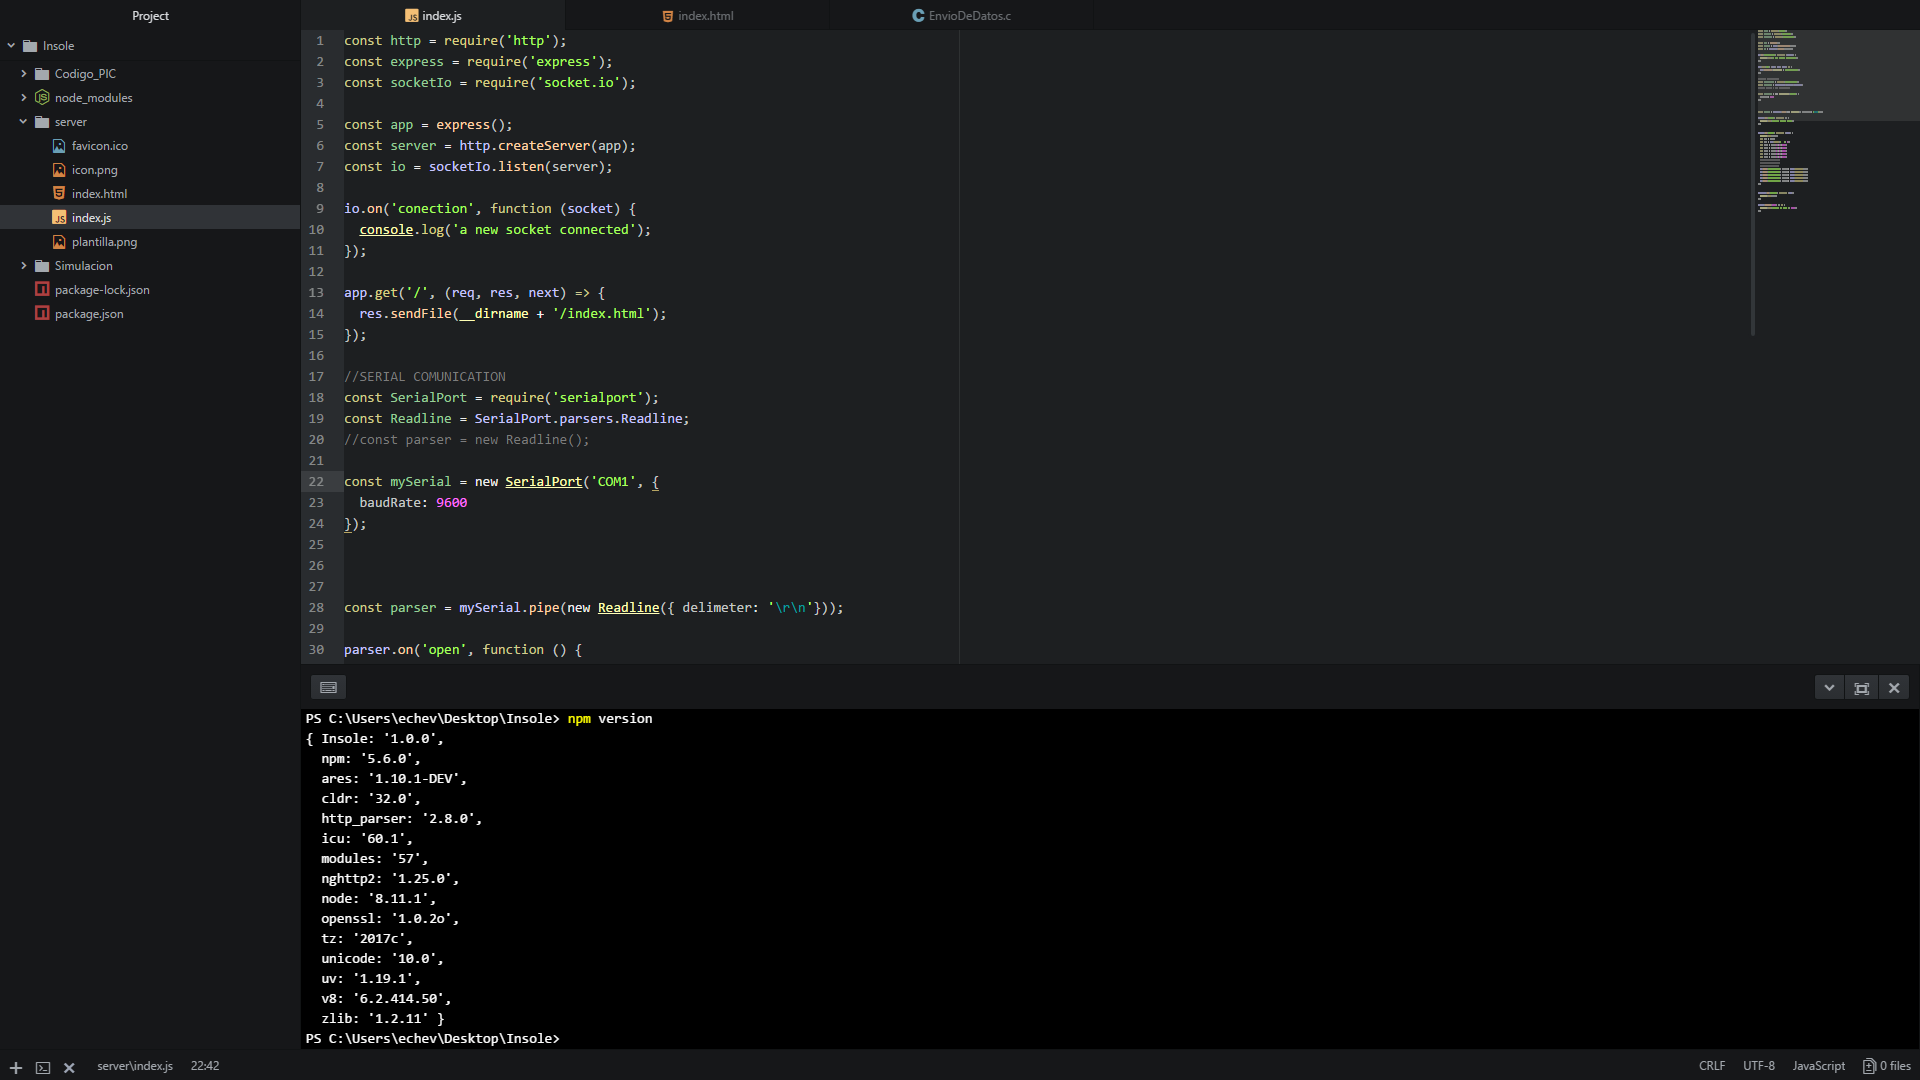
\includegraphics[width=1\textwidth]{./image/atom_image.png}}\\
    \subfloat[App Web desde cualquier navegador]{
   \label{fig:insoleweb}
    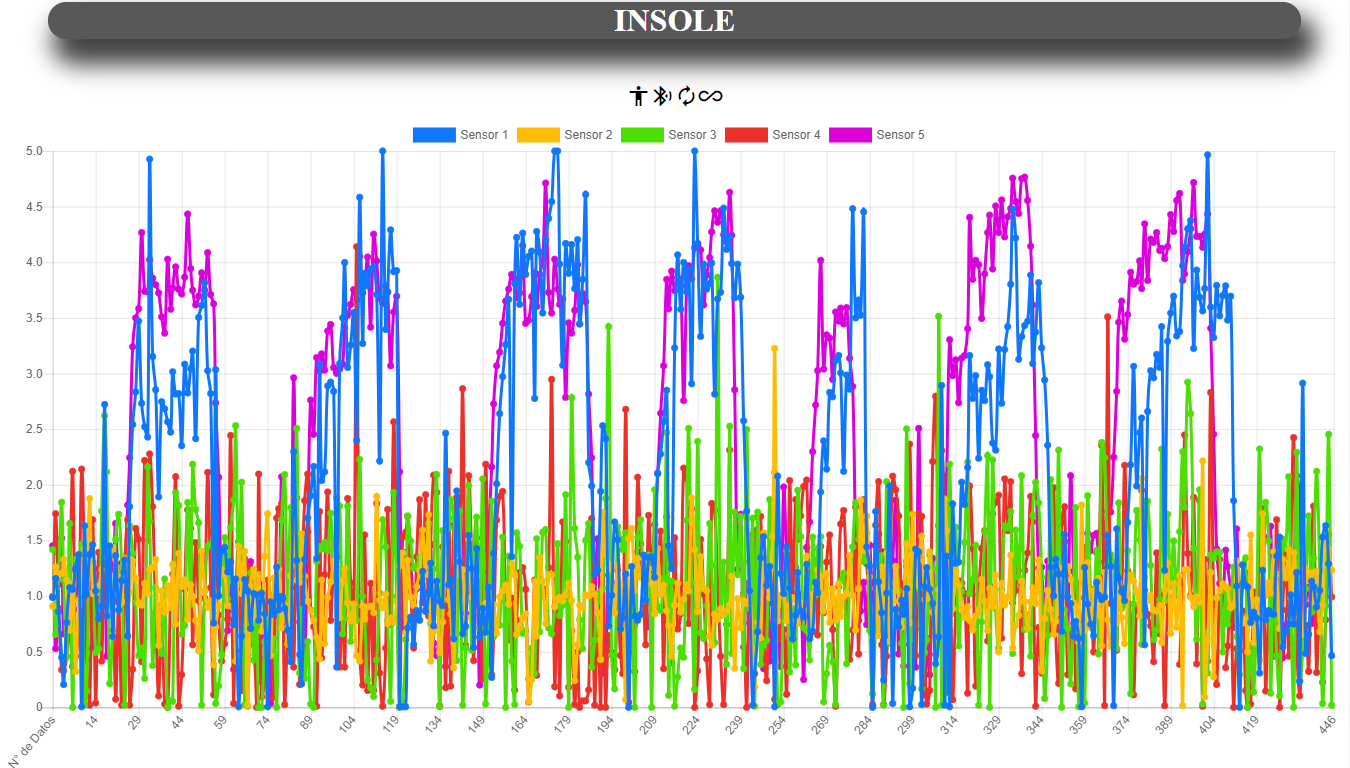
\includegraphics[width=1\textwidth]{./image/Insoleapp.png}}
 \caption{Software Utilizado para el desarrollo de la aplicación Web.}
 \label{fig:appWeb}
\end{figure}


\chapter{Resultados y Discusión} \label{sec:Resultados}

\section{Pruebas Realizadas con el Sistema en Funcionamiento}

Se realizaron 4 pruebas de esfuerzos diferentes entre ellas están las sentadillas con pesas de 25Kg, la maquina prensa sin pesas, correr por 10 metros y realizar 7 saltos; las dos primeras pruebas se hicieron en el gimnasio de la Universidad Tecnológica de Bolívar como se puede observar a continuación en la figura \ref{fig:Pruebas}.

\begin{figure}[H]
 \centering
  \subfloat[Sentadillas]{
   \label{fig:Sentadillas}
    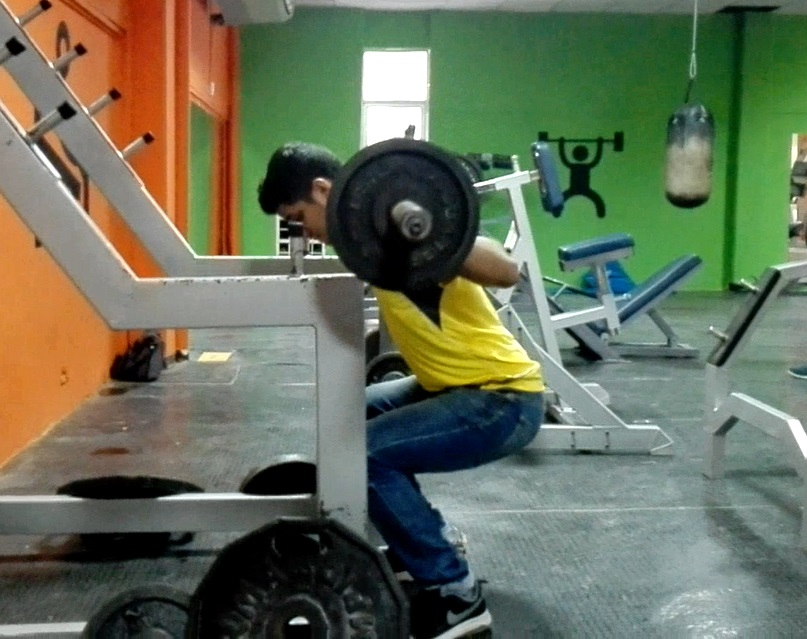
\includegraphics[width=0.244\textwidth]{./image/Sentadillas.jpg}}
    \subfloat[Prensa]{
   \label{fig:Prensa}
    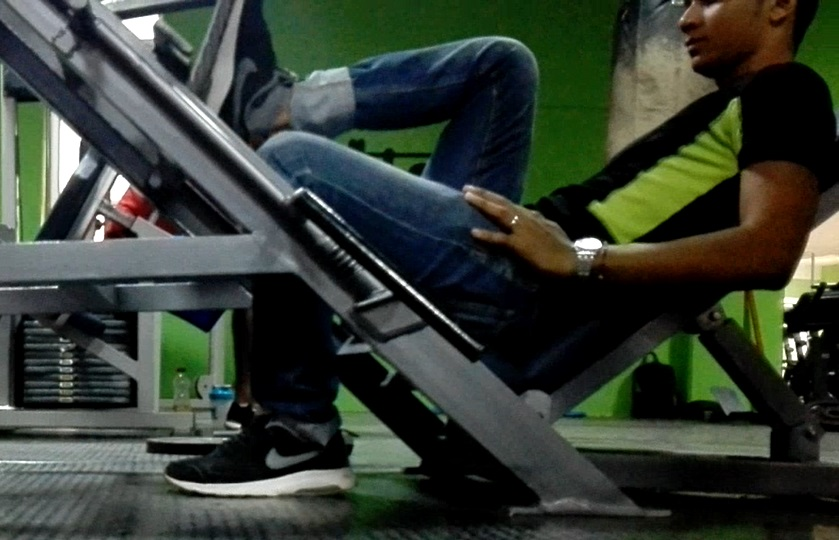
\includegraphics[width=0.3\textwidth]{./image/Prensa.jpg}}\\
    \subfloat[Correr]{
   \label{fig:Correr}
    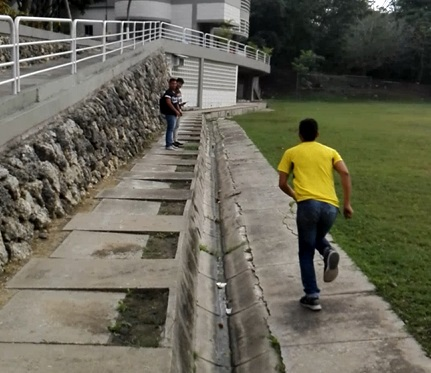
\includegraphics[width=0.3\textwidth]{./image/Correr.jpg}}
    \subfloat[Saltos]{
   \label{fig:Saltos}
    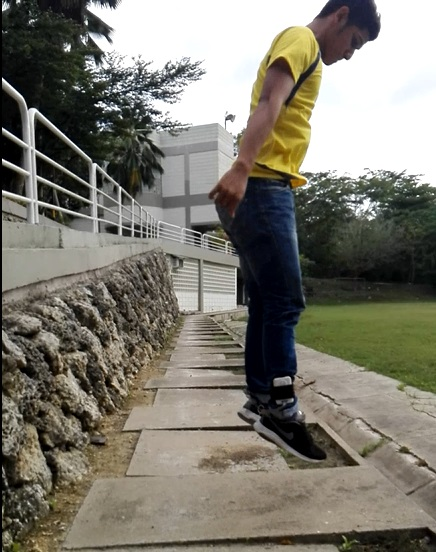
\includegraphics[width=0.205\textwidth]{./image/Saltos.jpg}}
 \caption{Pruebas realizadas.}
 \label{fig:Pruebas}
\end{figure}

\begin{table}[H]
\small
%\footnotesize
%\scriptsize
%\tiny
\begin{center}
\resizebox{10cm}{!} {
\begin{tabular}{| c | c | c | c | c | c | c | c | c | c | c | c |}
\hline
\multicolumn{6}{| c |}{\textbf{Sentadillas con 25Kg}} & \multicolumn{6}{| c |}{\textbf{Saltos}}\\
 \hline
\textbf{Sensor 1} & \textbf{Sensor 2} & \textbf{Sensor 3} & \textbf{Sensor 4} & \textbf{Sensor 5} & \textbf{Tiempo} & \textbf{Sensor 1} & \textbf{Sensor 2} & \textbf{Sensor 3} & \textbf{Sensor 4} & \textbf{Sensor 5} & \textbf{Tiempo}\\ 
 \hline
1,34 &	1,08 &	0,96 &	0,95 &	1,06 &	0,3 & 1,00 & 0,96 &	0,96 & 0,98 & 0,98 & 0,3\\
\hline
1,37 &	1,01 &	0,97 &	0,95 &	1,05 &	0,6 & 1,00 & 0,96 & 0,99 & 0,98 & 0,98 & 0,6\\
\hline
1,38 &	1,03 &	0,96 &	0,95 &	0,99 &	0,9 & 1,03 & 0,96 & 0,97 & 0,98 & 0,98 & 0,9\\
\hline
1,37 &	1,02 &	0,95 &	0,96 &	1,00 &	1,2 & 1,06 & 0,95 & 0,95 & 0,97 & 0,99 & 1,2\\
\hline
1,40 &	1,03 &	0,96 &	0,95 &	0,98 &	1,4 & 1,17 & 0,93 & 0,94 & 0,96 & 0,98 & 1,4\\
\hline
1,40 &	1,07 &	0,97 &	0,95 &	0,97 &	1,7 & 1,13 & 0,97 & 1,01 & 0,96 & 1,01 & 1,7\\
\hline
1,30 &	1,10 &	0,96 &	0,95 &	0,98 &	2,0 & 1,30 & 0,94 & 0,95 & 0,94 & 1,26 & 2,0\\
\hline
1,41 &	1,08 &	0,96 &	0,95 &	0,98 &	2,3 & 1,21 & 0,95 & 0,96 & 0,96 & 1,04 & 2,3\\
\hline
1,35 &	1,08 &	0,94 &	0,95 &	0,98 &	2,6 & 1,56 & 1,02 & 0,96 & 0,95 & 1,03 & 2,6\\
\hline
1,37 &	0,99 &	0,96 &	0,94 &	1,05 &	2,9 & 1,09 & 0,96 & 1,01 & 0,96 & 1,02 & 2,9\\
\hline
1,35 &	0,99 &	0,95 &	0,96 &	1,04 &	3,2 & 1,15 & 0,97 & 0,98 & 0,97 & 0,97 & 3,2\\
\hline
1,36 &	1,02 &	0,94 &	0,95 &	0,98 &	3,5 & 1,36 & 0,94 & 0,97 & 0,96 & 0,95 & 3,5\\
\hline
1,38 &	1,07 &	0,97 &	0,96 &	1,01 &	3,7 & 1,14 & 0,95 & 0,96 & 0,96 & 0,97 & 3,7\\
\hline
1,39 &	1,10 &	0,96 &	0,96 &	0,95 &	4,0 & 1,42 & 0,95 & 0,95 & 0,95 & 0,95 & 4,0\\
\hline
1,29 &	1,08 &	0,96 &	0,95 &	0,97 &	4,3 & 1,39 & 0,97 & 0,97 & 0,96 & 1,05 & 4,3\\
\hline
1,32 &	0,96 &	0,96 &	0,96 &	0,99 &	4,6 & 1,22 & 0,97 & 0,96 & 0,95 & 0,97 & 4,6\\
\hline
1,30 &	0,97 &	0,99 &	0,95 &	0,92 &	4,9 & 1,40 & 1,04 & 0,94 & 0,95 & 1,03 & 4,9\\
\hline
1,29 &	0,97 &	0,95 &	0,93 &	0,98 &	5,2 & 1,40 & 0,96 & 0,95 & 0,95 & 1,02 & 5,2\\
\hline
1,31 &	1,00 &	0,97 &	0,95 &	0,94 &	5,5 & 1,58 & 0,97 & 0,95 & 0,95 & 1,11 & 5,5\\
\hline
1,33 &	1,02 &	0,95 &	0,96 &	0,95 &	5,8 & 1,31 & 0,95 & 0,95 & 0,95 & 0,99 & 5,8\\
\hline
1,35 &	1,04 &	0,96 &	0,95 &	0,95 &	6,1 & 1,18 & 0,95 & 0,96 & 0,96 & 0,95 & 6,1\\
\hline
1,30 &	1,12 &	0,96 &	0,95 &	0,95 &	6,3 & 1,10 & 0,95 & 0,96 & 0,98 & 0,94 & 6,3\\
\hline
1,35 &	1,11 &	0,95 &	0,95 &	0,96 &	6,6 & 1,21 & 0,96 & 0,96 & 0,96 & 0,95 & 6,6\\
\hline
1,31 &	1,03 &	0,95 &	0,95 &	0,96 &	6,9 & 1,13 & 0,95 & 0,96 & 0,96 & 0,95 & 6,9\\
\hline
1,32 &	1,03 &	0,95 &	0,95 &	0,96 &	7,2 & 1,20 & 0,95 & 0,97 & 0,95 & 0,96 & 7,2\\
\hline
1,30 &	1,01 &	0,95 &	0,95 &	0,98 &	7,5 & 1,49 & 0,96 & 0,96 & 0,96 & 1,03 & 7,5\\
\hline
1,39 &	1,02 &	0,95 &	0,95 &	0,95 &	7,8 & 1,28 & 0,99 & 0,96 & 0,95 & 1,17 & 7,8\\
\hline
1,36 &	1,06 &	0,96 &	0,95 &	1,01 &	8,1 & 0,97 & 1,03 & 0,95 & 0,95 & 1,13 & 8,1\\
\hline
1,36 &	1,09 &	0,97 &	0,94 &	1,05 &	8,4 & 1,29 & 0,95 & 0,96 & 0,96 & 0,97 & 8,4\\
\hline
1,38 &	1,04 &	0,95 &	0,95 &	0,95 &	8,7 & 1,41 & 0,98 & 0,97 & 0,96 & 0,97 & 8,7\\
\hline
1,39 &	1,00 &	0,96 &	0,95 &	0,96 &	8,9 & 1,17 & 0,97 & 0,96 & 1,00 & 1,13 & 8,9\\
\hline
1,35 &	1,01 &	0,95 &	0,95 &	0,97 &	9,2 & 1,14 & 0,97 & 0,97 & 0,99 & 0,99 & 9,2\\
\hline
1,37 &	1,02 &	0,95 &	0,94 &	0,94 &	9,5 & 1,22 & 0,95 & 0,96 & 0,97 & 0,97 & 9,5\\
\hline
1,40 &	1,01 &	0,97 &	0,95 &	1,00 &	9,8 & 1,20 & 0,95 & 0,97 & 0,97 & 0,97 & 9,8\\
\hline
1,38 &	1,07 &	0,95 &	0,98 &	0,98 &	10,1 & 1,19 & 0,95 & 0,96 & 0,95 & 1,00 & 10,1\\
\hline
1,37 &	1,08 &	0,95 &	0,94 &	0,97 &	10,4 & 1,06 & 0,96 & 0,96 & 0,98 & 0,95 & 10,4\\
\hline
1,34 &	1,06 &	0,95 &	0,96 &	0,98 &	10,7 & 1,05 & 0,95 & 0,97 & 0,97 & 0,94 & 10,7\\
\hline
1,37 &	0,99 &	0,95 &	0,96 &	0,96 &	11,0 & 1,03 & 1,01 & 0,97 & 0,96 & 0,97 & 11,0\\
\hline
1,37 &	0,99 &	0,95 &	0,95 &	0,96 &	11,3 & 1,32 & 0,96 & 1,00 & 0,95 & 0,95 & 11,3\\
\hline
1,35 &	1,02 &	0,95 &	0,95 &	0,96 &	11,5 & 1,25 & 0,97 & 0,98 & 0,97 & 1,09 & 11,5\\
\hline
1,41 &	1,00 &	0,95 &	0,95 &	0,98 &	11,8 & 1,32 & 0,97 & 0,95 & 0,95 & 1,03 & 11,8\\
\hline
1,41 &	1,08 &	0,96 &	0,95 &	0,99 &	12,1 & 1,35 & 1,17 & 0,95 & 0,96 & 1,20 & 12,1\\
\hline
1,45 &	1,08 &	0,95 &	0,95 &	0,98 &	12,4 & 1,22 & 1,16 & 0,96 & 0,95 & 1,04 & 12,4\\
\hline
1,40 &	1,01 &	0,98 &	0,95 &	0,97 &	12,7 & 1,31 & 0,98 & 0,98 & 0,97 & 1,00 & 12,7\\
\hline
1,34 &	0,96 &	0,95 &	0,93 &	0,96 &	13,0 & 1,55 & 0,96 & 0,95 & 0,96 & 1,11 & 13,0\\
\hline
1,32 &	0,94 &	0,95 &	0,97 &	0,94 &	13,3 & 1,47 & 0,95 & 0,95 & 0,97 & 0,97 & 13,3\\
\hline
1,32 &	0,97 &	0,95 &	0,96 &	0,95 &	13,6 & 1,41 & 0,94 & 0,95 & 0,95 & 0,98 & 13,6\\
\hline
1,44 &	0,99 &	0,95 &	0,94 &	0,94 &	13,8 & 1,32 & 0,95 & 0,95 & 0,95 & 0,97 & 13,8\\
\hline
1,40 &	1,04 &	0,95 &	0,95 &	0,96 &	14,1 & 1,28 & 0,96 & 0,96 & 0,97 & 0,96 & 14,1\\
\hline
1,38 &	1,08 &	0,94 &	0,95 &	0,97 &	14,4 & 1,22 & 0,96 & 0,96 & 0,99 & 0,97 & 14,4\\
\hline
1,40 &	1,04 &	0,95 &	0,95 &	0,96 &	14,7 & 1,20 & 0,95 & 0,95 & 0,96 & 0,95 & 14,7\\
\hline
1,37 &	1,00 &	0,95 &	0,94 &	0,94 &	15,0 & 1,48 & 0,95 & 0,95 & 0,97 & 1,23 & 15,0\\
\hline
1,38 &	1,01 &	0,95 &	0,95 &	0,93 &	15,3 & 1,34 & 0,95 & 0,95 & 0,95 & 0,97 & 15,3\\
\hline
1,37 &	1,00 &	0,95 &	0,96 &	0,94 &	15,6 & 1,44 & 0,96 & 0,97 & 0,99 & 1,01 & 15,6\\
\hline
1,37 &	1,01 &	0,95 &	0,95 &	0,96 &	15,9 & 1,64 & 0,95 & 0,95 & 0,95 & 1,21 & 15,9\\
\hline
1,38 &	1,01 &	0,95 &	0,95 &	0,95 &	16,2 & 1,36 & 0,95 & 0,95 & 0,96 & 1,11 & 16,2\\
\hline
1,44 &	1,03 &	0,95 &	0,95 &	0,97 &	16,4 & 1,74 & 0,99 & 0,96 & 0,96 & 1,01 & 16,4\\
\hline
1,39 &	1,07 &	0,96 &	0,95 &	0,98 &	16,7 & 1,59 & 0,96 & 0,96 & 0,98 & 1,09 & 16,7\\
\hline
1,36 &	1,04 &	0,95 &	0,96 &	0,97 &	17,0 & 1,43 & 0,96 & 0,95 & 0,97 & 0,99 & 17,0\\
\hline
1,36 &	0,97 &	0,95 &	0,96 &	0,95 &	17,3 & 1,32 & 0,92 & 0,96 & 0,95 & 0,94 & 17,3\\
\hline
1,33 &	0,97 &	0,93 &	0,95 &	0,98 &	17,6 & 1,26 & 0,95 & 0,98 & 0,96 & 0,95 & 17,6\\
\hline
1,37 &	0,99 &	0,95 &	0,97 &	0,93 &	17,9 & 1,27 & 0,95 & 0,97 & 0,96 & 0,95 & 17,9\\
\hline
1,36 &	1,01 &	0,95 &	0,96 &	0,99 &	18,2 & 1,30 & 0,95 & 0,96 & 1,02 & 1,07 & 18,2\\
\hline
1,38 &	0,98 &	0,95 &	0,95 &	0,97 &	18,5 & 1,36 & 0,96 & 0,95 & 0,96 & 1,00 & 18,5\\
\hline
1,40 &	1,00 &	0,93 &	0,95 &	0,97 &	18,8 & 1,37 & 0,95 & 0,96 & 0,95 & 1,00 & 18,8\\
\hline
1,39 &	1,01 &	0,95 &	0,97 &	0,98 &	19,0 & 1,32 & 0,94 & 0,95 & 0,94 & 0,95 & 19,0\\
\hline
1,39 &	1,11 &	0,95 &	0,95 &	0,97 &	19,3 & 1,55 & 0,98 & 0,95 & 0,97 & 1,11 & 19,3\\
\hline
1,42 &	1,03 &	0,95 &	0,95 &	1,01 &	19,6 & 1,53 & 0,99 & 0,95 & 0,95 & 1,28 & 19,6\\
\hline
1,43 &	1,02 &	0,95 &	0,95 &	0,99 &	19,9 & 1,50 & 0,98 & 0,97 & 0,96 & 1,27 & 19,9\\
\hline
1,38 &	1,01 &	0,95 &	0,95 &	0,94 &	20,2 & 1,36 & 0,96 & 0,96 & 0,95 & 1,15 & 20,2\\
\hline
1,38 &	1,01 &	0,94 &	0,96 &	0,98 &	20,5 & 1,44 & 0,98 & 0,96 & 0,97 & 0,96 & 20,5\\
\hline
1,40 &	1,02 &	0,95 &	0,95 &	0,95 &	20,8 & 1,45 & 0,96 & 0,95 & 0,95 & 0,98 & 20,8\\
\hline
1,39 &	1,00 &	0,95 &	0,96 &	1,00 &	21,1 & 1,22 & 0,96 & 0,95 & 0,97 & 1,07 & 21,1\\
\hline
1,42 &	1,01 &	0,95 &	0,95 &	0,96 &	21,3 & 1,26 & 0,95 & 0,96 & 1,00 & 1,36 & 21,3\\
\hline
1,41 &	1,06 &	0,95 &	0,95 &	1,01 &	21,6 & 1,34 & 0,95 & 0,95 & 0,97 & 1,20 & 21,6\\
\hline
1,44 &	1,02 &	0,95 &	0,96 &	1,01 &	21,9 & 1,23 & 0,95 & 0,95 & 0,97 & 1,11 & 21,9\\
\hline
1,41 &	1,06 &	0,97 &	0,97 &	0,97 &	22,2 & 1,17 & 0,96 & 0,96 & 0,97 & 1,00 & 22,2\\
\hline
1,39 &	1,03 &	0,96 &	0,94 &	0,97 &	22,5 & 1,26 & 0,95 & 0,97 & 0,96 & 0,96 & 22,5\\
\hline
1,37 &	1,01 &	0,95 &	0,95 &	0,99 &	22,8 & 1,20 & 0,97 & 0,95 & 0,96 & 0,97 & 22,8\\
\hline
1,41 &	1,02 &	0,95 &	0,97 &	0,94 &	23,1 & 1,19 & 0,95 & 0,95 & 0,99 & 0,99 & 23,1\\
\hline
1,40 &	0,99 &	0,95 &	0,95 &	0,92 &	23,4 & 1,20 & 0,97 & 0,96 & 0,96 & 0,95 & 23,4\\
\hline
1,43 &	1,04 &	0,95 &	0,95 &	0,98 &	23,7 & 1,32 & 0,97 & 0,99 & 0,98 & 1,07 & 23,7\\
\hline
1,44 &	1,07 &	0,95 &	0,96 &	1,04 &	23,9 & 1,91 & 1,01 & 0,95 & 0,94 & 1,26 & 23,9\\
\hline
1,43 &	1,03 &	0,95 &	0,95 &	1,02 &	24,2 & 1,55 & 0,97 & 0,95 & 0,96 & 1,23 & 24,2\\
\hline
1,40 &	1,03 &	0,95 &	0,95 &	0,95 &	24,5 & 1,41 & 0,97 & 0,96 & 0,96 & 1,17 & 24,5\\
\hline
1,36 &	1,01 &	0,96 &	0,95 &	0,97 &	24,8 & 1,83 & 1,01 & 0,96 & 0,94 & 1,01 & 24,8\\
\hline
1,39 &	1,02 &	0,95 &	0,97 &	0,97 &	25,1 & 1,74 & 0,96 & 0,95 & 0,96 & 1,09 & 25,1\\
\hline
1,41 &	1,01 &	0,95 &	0,96 &	0,95 &	25,4 & 1,31 & 0,95 & 0,96 & 0,96 & 1,03 & 25,4\\
\hline
1,42 &	1,05 &	0,95 &	0,95 &	0,99 &	25,7 & 1,32 & 0,95 & 0,96 & 0,96 & 1,76 & 25,7\\
\hline
1,45 &	1,12 &	0,94 &	0,95 &	1,03 &	26,0 & 1,39 & 0,95 & 0,95 & 0,95 & 0,96 & 26,0\\
\hline
1,40 &	1,17 &	0,95 &	0,95 &	1,02 &	26,2 & 1,12 & 0,95 & 0,96 & 0,95 & 0,97 & 26,2\\
\hline
1,48 &	1,02 &	0,95 &	0,94 &	1,05 &	26,5 & 1,33 & 0,94 & 0,97 & 0,97 & 1,25 & 26,5\\
\hline
1,49 &	1,00 &	0,95 &	0,95 &	0,96 &	26,8 & 1,31 & 0,95 & 0,94 & 0,96 & 1,07 & 26,8\\
\hline
1,42 &	0,99 &	0,95 &	0,97 &	1,03 &	27,1 & 1,30 & 0,96 & 0,96 & 1,00 & 1,04 & 27,1\\
\hline
1,34 &	1,01 &	0,95 &	0,96 &	1,14 &	27,4 & 1,28 & 0,95 & 0,96 & 0,97 & 1,03 & 27,4\\
\hline
1,43 &	0,99 &	0,95 &	0,95 &	1,01 &	27,7 & 1,13 & 0,95 & 0,96 & 0,98 & 1,06 & 27,7\\
\hline
1,48 &	1,11 &	0,95 &	0,97 &	1,08 &	28,0 & 1,38 & 0,95 & 0,96 & 0,95 & 0,96 & 28,0\\
\hline
1,50 &	1,06 &	0,95 &	0,95 &	1,00 &	28,3 & 1,96 & 1,00 & 0,94 & 0,94 & 1,21 & 28,3\\
\hline
1,43 &	1,11 &	0,96 &	0,95 &	1,00 &	28,6 & 1,83 & 0,94 & 0,95 & 0,95 & 1,28 & 28,6\\
\hline
1,39 &	1,02 &	0,95 &	0,96 &	0,94 &	28,8 & 1,53 & 0,95 & 0,95 & 0,96 & 1,13 & 28,8\\
\hline
1,37 &	0,98 &	0,95 &	0,98 &	1,24 &	29,1 & 1,49 & 0,99 & 1,01 & 0,97 & 1,00 & 29,1\\
\hline
1,41 &	1,02 &	0,96 &	0,95 &	0,97 &	29,4 & 1,30 & 0,97 & 1,00 & 0,96 & 0,93 & 29,4\\
\hline
1,35 &	1,03 &	0,94 &	0,95 &	0,93 &	29,7 & 1,28 & 0,96 & 1,00 & 0,97 & 0,95 & 29,7\\
\hline
1,55 &	1,03 &	0,95 &	0,96 &	0,98 &	30,0 & 1,13 & 0,95 & 0,99 & 1,06 & 0,99 & 30,0\\
 \hline
\end{tabular}
}
\caption{Valores obtenidos en las pruebas de Sentadillas con 25Kg de peso y 7 Saltos durante 30 segundos.}
\label{Table:Sentadillas_y_Saltos}
\end{center}
\end{table}

%\begin{table}[H]
%\small
%\footnotesize
%\scriptsize
%\tiny
%\begin{center}
%\resizebox{9cm}{!} {
%\begin{tabular}{| c | c | c | c | c | c |}
%\hline
%\multicolumn{6}{| c |}{\textbf{Correr}}\\
% \hline
%\textbf{Sensor 1} & \textbf{Sensor 2} & \textbf{Sensor 3} & \textbf{Sensor 4} & \textbf{Sensor 5} & \textbf{Tiempo}\\ 
% \hline
%1,42 & 0,97 & 0,94 & 0,96 & 1,18 & 0,3\\
%\hline
%1,49 & 0,99 & 0,96 & 0,95 & 1,18 & 0,6\\
%\hline
%1,46 & 0,99 & 0,95 & 0,96 & 1,18 & 0,9\\
%\hline
%1,43 & 1,02 & 0,95 & 0,96 & 1,17 & 1,2\\
%\hline
%1,44 & 0,98 & 0,97 & 0,96 & 1,17 & 1,4\\
%\hline
%1,45 & 0,99 & 0,95 & 0,96 & 1,16 & 1,7\\
%\hline
%0,96 & 0,96 & 0,98 & 0,96 & 1,16 & 2,0\\
%\hline
%1,57 & 0,98 & 0,98 & 0,96 & 0,97 & 2,3\\
%\hline
%1,38 & 0,97 & 0,97 & 0,96 & 1,05 & 2,6\\
%\hline
%1,53 & 1,05 & 1,16 & 1,44 & 1,06 & 2,9\\
%\hline
%1,34 & 0,95 & 0,95 & 0,96 & 1,06 & 3,2\\
%\hline
%1,38 & 0,97 & 0,95 & 0,96 & 0,97 & 3,5\\
%\hline
%1,53 & 0,95 & 0,97 & 0,95 & 0,94 & 3,7\\
%\hline
%1,35 & 0,95 & 0,94 & 0,96 & 1,00 & 4,0\\
%\hline
%1,76 & 1,03 & 1,06 & 1,35 & 1,22 & 4,3\\
%\hline
%1,44 & 0,95 & 0,95 & 0,96 & 1,15 & 4,6\\
%\hline
%1,47 & 0,97 & 0,97 & 0,96 & 0,96 & 4,9\\
%\hline
%1,49 & 0,96 & 0,99 & 0,96 & 0,92 & 5,2\\
%\hline
%1,44 & 0,98 & 0,95 & 0,96 & 0,97 & 5,5\\
%\hline
%1,47 & 0,97 & 0,96 & 0,95 & 0,96 & 5,8\\
%\hline
%1,49 & 0,95 & 0,95 & 0,95 & 1,04 & 6,1\\
%\hline
%1,44 & 0,96 & 0,95 & 0,96 & 1,01 & 6,3\\
%\hline
%1,62 & 1,03 & 1,15 & 0,97 & 1,00 & 6,6\\
%\hline
%1,45 & 0,96 & 0,96 & 0,95 & 1,12 & 6,9\\
%\hline
%1,49 & 0,95 & 0,94 & 0,96 & 0,94 & 7,2\\
%\hline
%1,55 & 0,93 & 0,95 & 0,96 & 1,00 & 7,5\\
%\hline
%1,47 & 0,96 & 0,96 & 0,95 & 0,96 & 7,8\\
%\hline
%1,46 & 0,96 & 0,97 & 1,04 & 1,53 & 8,1\\
%\hline
%1,38 & 0,95 & 0,95 & 0,96 & 1,03 & 8,4\\
%\hline
%1,43 & 0,96 & 0,95 & 0,96 & 1,03 & 8,7\\
%\hline
%1,77 & 1,04 & 1,11 & 1,07 & 1,09 & 8,9\\
%\hline
%1,40 & 0,95 & 0,95 & 0,96 & 1,02 & 9,2\\
%\hline
%1,35 & 0,96 & 1,01 & 0,96 & 0,99 & 9,5\\
%\hline
%1,87 & 0,96 & 1,09 & 0,94 & 1,06 & 9,8\\
%\hline
%1,30 & 0,95 & 0,96 & 0,95 & 1,12 & 10,1\\
%\hline
%1,48 & 0,96 & 0,96 & 0,96 & 1,03 & 10,4\\
%\hline
%1,75 & 0,97 & 1,05 & 0,95 & 1,01 & 10,7\\
%\hline
%1,53 & 0,95 & 0,95 & 0,96 & 1,15 & 11,0\\
%\hline
%1,52 & 0,95 & 0,95 & 1,00 & 1,47 & 11,3\\
%\hline
%1,58 & 0,95 & 0,96 & 0,95 & 1,13 & 11,5\\
%\hline
%1,56 & 0,96 & 0,96 & 0,96 & 0,98 & 11,8\\
%\hline
%1,67 & 0,97 & 0,99 & 0,95 & 1,14 & 12,1\\
%\hline
%1,65 & 0,96 & 0,95 & 0,96 & 1,11 & 12,4\\
%\hline
%1,68 & 0,96 & 0,94 & 0,96 & 0,99 & 12,7\\
%\hline
%1,64 & 0,96 & 0,95 & 0,96 & 1,13 & 13,0\\
%\hline
%1,49 & 0,96 & 0,96 & 0,96 & 1,01 & 13,3\\
%\hline
%1,56 & 0,99 & 1,03 & 1,02 & 1,10 & 13,6\\
%\hline
%1,58 & 0,97 & 0,97 & 0,96 & 1,16 & 13,8\\
%\hline
%1,59 & 0,96 & 0,95 & 0,96 & 1,01 & 14,1\\
%\hline
%1,64 & 0,94 & 0,96 & 0,95 & 1,14 & 14,4\\
%\hline
%1,40 & 0,98 & 0,94 & 0,95 & 1,04 & 14,7\\
%\hline
%1,67 & 0,96 & 0,95 & 1,08 & 1,59 & 15,0\\
%\hline
%1,62 & 0,95 & 0,95 & 0,95 & 1,24 & 15,3\\
%\hline
%1,63 & 0,98 & 0,95 & 0,96 & 1,00 & 15,6\\
%\hline
%1,60 & 0,97 & 1,13 & 0,95 & 0,99 & 15,9\\
%\hline
%1,40 & 0,98 & 0,95 & 0,95 & 1,30 & 16,2\\
%\hline
%1,72 & 0,97 & 0,95 & 0,96 & 0,99 & 16,4\\
%\hline
%1,23 & 0,97 & 0,95 & 0,96 & 1,01 & 16,7\\
% \hline
%\end{tabular}
%}
%\caption{Valores obtenidos en la prueba de Correr.}
%\label{Table:Correr}
%\end{center}
%\end{table}

%\begin{figure}[H]
%\centering
%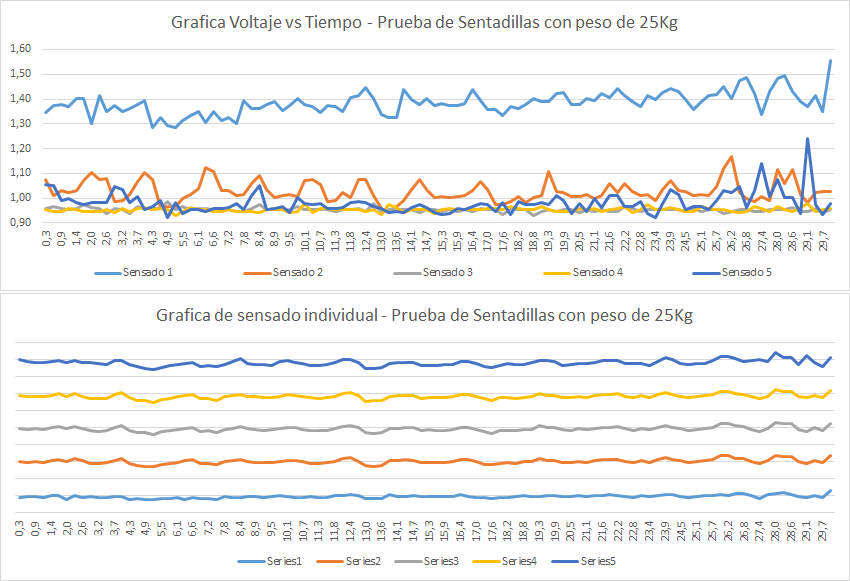
\includegraphics[width=1\textwidth]{./image/Grafica_Sentadillas.png}
%\caption{Gráfica de la prueba de sentadillas durante 30 segundos con pesas de 25Kg.}
%\label{fig:Grafica_Sentadillas}
%\end{figure}

\begin{figure}[H]
\centering
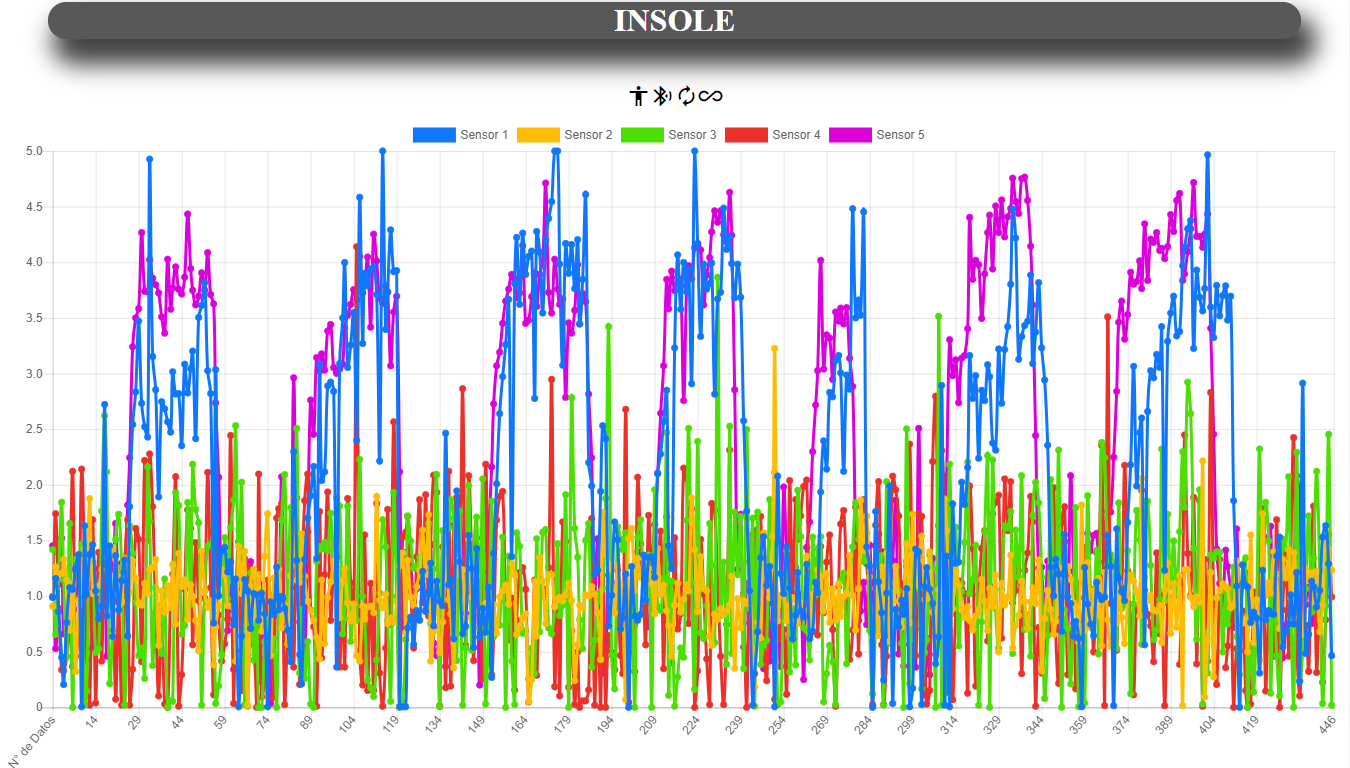
\includegraphics[width=1\textwidth]{./image/Insoleapp.png}
\caption{Gráfica de la prueba de Saltos durante 30 segundos.}
\label{fig:Grafica_Saltos}
\end{figure}

\begin{wrapfigure}{r}{0.2\linewidth}
\centering

\includegraphics[width=0.15\textwidth]{./image/Plantilla_Derecha.png}
\caption{Plantilla derecha con la ubicación de cada sensor.}
\label{fig:Plantilla_derecha}
\end{wrapfigure}

Se llevaron acabo pruebas para evaluar la comodidad y usabilidad del sistema, estas pruebas fueron usar la plantilla por debajo y por encima de la plantilla del calzado concluyendo así que para mayor comodidad del sistema, la plantilla diseñada debe ser usada por debajo de la plantilla del calzado deportivo.

Los resultados de las pruebas son trazados en la figura \ref{fig:Grafica_Saltos} se pueden observar los 7 valores por encima del promedio en la gráfica obtenida de la prueba de saltos \ref{fig:Saltos} observando los 7 saltos que fueron realizados en la prueba, se notan variaciones en el sensor numero 1 el cual esta ubicado en el dedo grueso y el sensor 5 ubicado en el talón.

El valor máximo de presión se registra en el centro del talón y el dedo grueso, en la practica de saltos primero se toma impulso sobre cargando la parte superior del pie para el salto y al final del movimiento sobre cargando la parte central del talón que es donde descansa la mayor parte del peso del cuerpo.

%\begin{figure}[H]
%\centering
%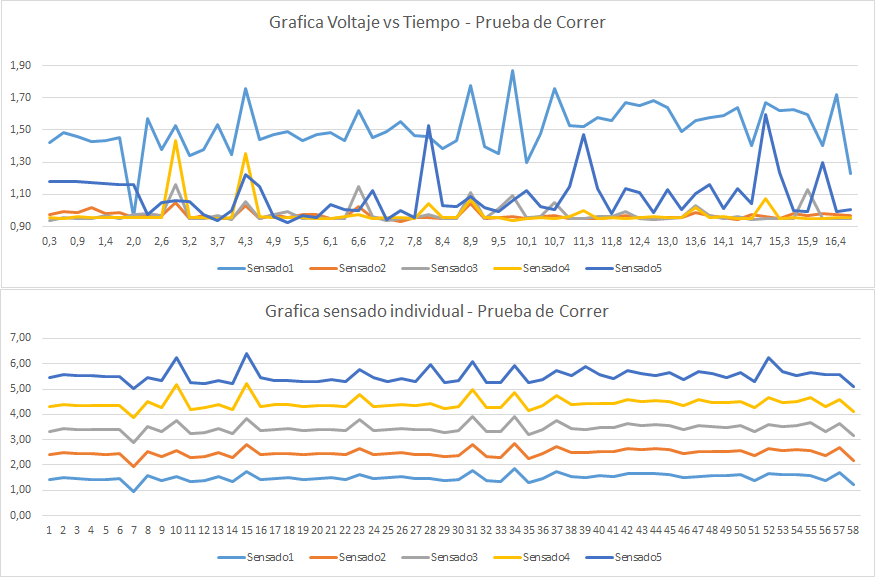
\includegraphics[width=1\textwidth]{./image/Grafica_Correr.png}
%\caption{Gráfica de la prueba de correr.}
%\label{fig:Grafica_Correr}
%\end{figure}




\chapter{Conclusiones y Recomendaciones} \label{sec:Conclusiones}

El sistema diseñado es apropiado para las características planteadas (portabilidad, tamaño, remoto, consumo, biocompatibilidad). Sin embargo, al momento de su implementación la principal complejidad de este fue la calibración de cada sensor debido a que cada sensor no cumplía con su curva característica la cual está definida por el fabricante como se observa en la figura \ref{fig:Curvas}. 

En cuanto al diseño electrónico se realizaron pruebas muy concisas que nos permitieron tener un bosquejo de las medidas aproximadas para cada sensor (figura \ref{fig:Comportamiento}), esto fue posible por las diferentes pruebas realizadas para que la ganancia del circuito sea apropiada para que abarque el rango de 1 a 5 Voltios.

El sistema presentado proporciona medidas simultaneas de presión de 5 sensores ubicados de la siguiente manera: sensor 1 corresponde al dedo grueso, sensor 2 y 3 al primer y quinto metatarsiano respectivamente, el sensor 4 en la zona lateral de la planta y por ultimo el sensor 5 ubicado en el talón. El análisis de los datos se puede llevar a cabo con la aplicación web que gráfica las variaciones de presión en tiempo real, de esta forma el sujeto obtiene una retroalimentacion inmediata sobre su patología la cual puede ser corregida en el mismo instante.

Este sistema puede ser utilizado en diferentes tipos de aplicaciones como pueden ser la elección de zapatos mas apropiados, rehabilitación de diferentes lesiones, estudio de patrones a la hora de caminar por personas afectadas por enfermedades como Parkinson y Diabetes.

\chapter{Anexos}\label{sec:Anexos}

\section{Diagrama de Bloques del sistema completo}

\begin{figure*}[h!]
\centering
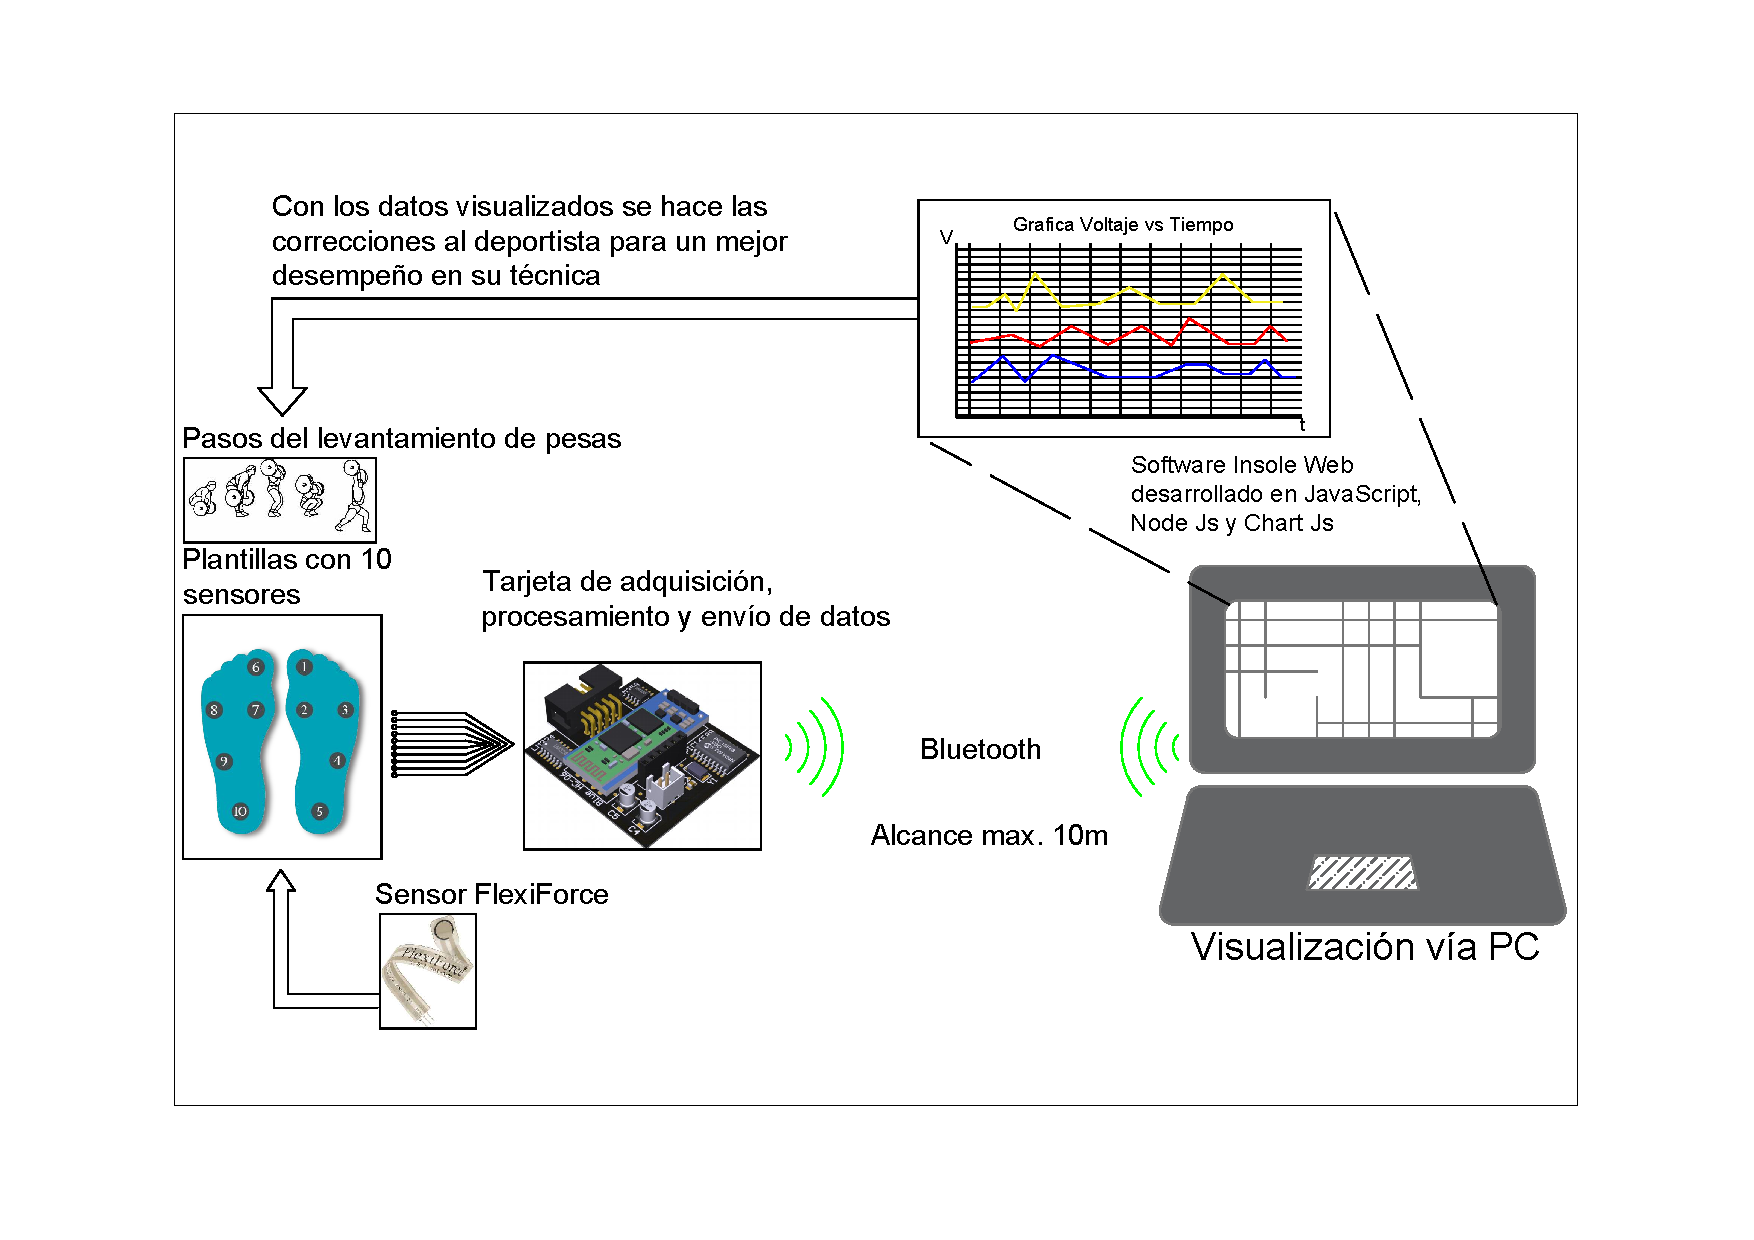
\includegraphics[width=1\textwidth]{./Documentos_PDF/Diagrama_de_Bloques_sistema_Insole.pdf}
\caption{Diagrama de Bloques del sistema de adquisición de datos.}
\label{fig:DiagramaBloque}
\end{figure*}

\newpage
\section{Código para el Microcontrolador PIC16F88}

\begin{lstlisting}[style=C]
///////////////////////////////////////////////////////////////////////////////////////////
//                                                                                       //
//                               PIC-Sensor_Plantilla1-UTB                               //
//                         @author: Ivan Dario Echeverry Mancera                         //
//                                                                                       //
///////////////////////////////////////////////////////////////////////////////////////////
//                                                                                       //
//              uControlador: PIC16F88                     Lenguaje: C                   //
//           Oscilacionde cristal (Xtal): 12MHz                                          //
//                                                                                       //
///////////////////////////////////////////////////////////////////////////////////////////

unsigned int Sensado1;
unsigned int Sensado2;
unsigned int Sensado3;
unsigned int Sensado4;
unsigned int Sensado5;

char texto1[20];
char texto2[20];
char texto3[20];
char texto4[20];
char texto5[20];

void main() 
{

	TrisA.b0=1;
    TrisA.b1=1; 
    TrisA.b2=1;
    TrisA.b3=1;
    TrisA.b4=1;
    Trisb.b2=1;//RX entrada
  	Trisb.b5=0;//TX salida
    
  	ADC_init();
  	UART1_init(9600);
    
  	Delay_ms(1000); 
}

while(1)
{

	Sensado1 = ADC_Read(0);
	wordtostr(Sensado1,texto1);
    
	Sensado2 = ADC_Read(1);
	wordtostr(Sensado2,texto2);
    
	Sensado3 = ADC_Read(2);
	wordtostr(Sensado3,texto3);
    
	Sensado4 = ADC_Read(3);
	wordtostr(Sensado4,texto4);
    
	Sensado5 = ADC_Read(4);
	wordtostr(Sensado5,texto5);

                           UART1_Write_Text(texto1);
                           UART1_Write_Text(" ");

                           UART1_Write_Text(texto2);
                           UART1_Write_Text(" ");

                           UART1_Write_Text(texto3);
                           UART1_Write_Text(" ");

                           UART1_Write_Text(texto4);
                           UART1_Write_Text(" ");

                           UART1_Write_Text(texto5);
                           UART1_Write(0x0A);

 Delay_ms(100);
}

\end{lstlisting}

\newpage
\section{Código HTML}

\begin{lstlisting}[style=HTML5]
<!DOCTYPE html>
<html>
  <head>
    <link rel="stylesheet" href="https://cdnjs.cloudflare.com/ajax/libs/font-awesome/4.7.0/css/font-awesome.min.css">
    <link href="https://fonts.googleapis.com/icon?family=Material+Icons" rel="stylesheet">
    <link rel="icon" type="image/png" href="icon.png" />
    <meta charset="utf-8">
    <title>Insole</title>
    
    <style>
  #parrafo {
    background-color:#585858;
    margin: 10px;
    padding: 20px;
    -webkit-box-shadow: 10px 20px 39px 6px rgba(0,0,0,0.75);
    -moz-box-shadow: 10px 20px 39px 6px rgba(0,0,0,0.75);
    box-shadow: 10px 20px 39px 6px rgba(0,0,0,0.75);
    border-radius: 20px 20px 20px 20px;
    -moz-border-radius: 20px 20px 20px 20px;
    -webkit-border-radius: 20px 20px 20px 20px;
    border: 0px solid #000000;
  }
  #izq {
    background-color:#FFFFFF;
    margin: 10px;
    padding: 0px;
    -webkit-box-shadow: 10px 20px 30px 6px rgba(0,0,0,0.75);
    -moz-box-shadow: 10px 20px 30px 6px rgba(0,0,0,0.75);
    box-shadow: 10px 20px 30px 6px rgba(0,0,0,0.75);
    border-radius: 20px 20px 20px 20px;
    -moz-border-radius: 20px 20px 20px 20px;
    -webkit-border-radius: 20px 20px 20px 20px;
    border: 0px solid #000000;
  }
  #titulo {
    background-color:#585858;
    margin: 20px;
    -webkit-box-shadow: 10px 20px 39px 6px rgba(0,0,0,0.75);
    -moz-box-shadow: 10px 20px 39px 6px rgba(0,0,0,0.75);
    box-shadow: 10px 20px 39px 6px rgba(0,0,0,0.75);
    border-radius: 20px 20px 20px 20px;
    -moz-border-radius: 20px 20px 20px 20px;
    -webkit-border-radius: 20px 20px 20px 20px;
    border: 0px solid #000000;
  }
  #iconos {
    display: block;
    margin: 0px;
    padding: 0px;
    border: 0px;
    font-size: 2em;
    -webkit-margin-before: 0.1em;
    -webkit-margin-after: 0.1em;
    -webkit-margin-start: 0px;
    -webkit-margin-end: 0px;
    font-weight: bold;
  }
  #titulografica {
    background-color:#585858;
    margin: 0px;
    padding: 20px;
    border-radius: 20px 20px 0px 0px;
    -moz-border-radius: 20px 20px 0px 0px;
    -webkit-border-radius: 20px 20px 0px 0px;
  }
  #Der {
    margin: 0px;
    padding: 150px 0px 0px 0px;
  }
  </style>
  
  </head>
  <body>
  
    <div id="titulo">
    <h1 align=center><font color="White">INSOLE</font></h1>
    </div>
    <h1 id="iconos" align="center"><i class="material-icons md-16">accessibility</i><i class="material-icons md-16">bluetooth_searching</i><i class="material-icons md-16">autorenew</i><i class="material-icons md-16">all_inclusive</i></h1>
    <div class="box">
      <div class="container">
        <div id="izq" style="float: left; width: 83%">
          <p id="titulografica"><font color="White">Grafica plantilla derecha - Insole</font></p>
          <canvas id="myCanvas" style="display: block; width:100%"></canvas>
        </div>
      </div>
      
        <script src="https://cdnjs.cloudflare.com/ajax/libs/Chart.js/2.7.2/Chart.min.js" charset="utf-8"></script>
        <script src="/socket.io/socket.io.js" charset="utf-8"></script>
        <script>
          var socket = io();
          var chartOptions = {
            scales: {
              xAxes: [{
                scaleLabel: {
                  display: true,
                  labelString: "Numero de Datos Obtenidos"
                }
              }],
              yAxes: [{
                ticks: {
                  min: 0.8,
                  max: 5,
                  stepSize: 0.1
                },
                scaleLabel: {
                  display: true,
                  labelString: "Voltaje [V]"
                }
              }]
            },
            responsive: false
          };
          
          var ctx = document.getElementById("myCanvas").getContext('2d');
          var myChart = new Chart(ctx, {
            type: 'line',
            data: {
              labels: [],
              datasets: [{
                label: "Sensor 1",
                fill: false,
                borderColor: 'rgb(16, 119, 251)',
                backgroundColor: 'rgb(16, 119, 251)',
                data: []
              },{
                label: "Sensor 2",
                fill: false,
                borderColor: "rgb(254, 189, 5)",
                backgroundColor: "rgb(254, 189, 5)",
                data: []
              }, {
                label: "Sensor 3",
                fill: false,
                borderColor: "rgb(77, 222, 5)",
                backgroundColor: "rgb(77, 222, 5)",
                data: []
              }, {
                label: "Sensor 4",
                fill: false,
                borderColor: "rgb(234, 49, 42)",
                backgroundColor: "rgb(234, 49, 42)",
                data: []
              }, {
                label: "Sensor 5",
                fill: false,
                borderColor: "rgb(218, 1, 218)",
                backgroundColor: "rgb(218, 1, 218)",
                data: []
              }]
            },
            options: chartOptions
          });
          
          var counter = 0;
          var DATA_LIMIT = 300;
          var labels = myChart.data.labels;
          socket.on('sen:data', function (senArray) {
            labels.push(counter++);
            var isFull = labels.length === DATA_LIMIT;
            if(isFull) labels.shift();
            senArray.forEach((sen, index) => {
              var chartData = myChart.data.datasets[index];
              chartData.data.push(sen);
              if(isFull) chartData.data.shift();
            });
            
            myChart.update();
          });
          </script>
          
        <div class="container">
          <div id="Der" style="float: right; width: 14%">
            <img src="plantilla.png" style="margin-left: auto; margin-right: auto; display: block; width: 70%;"/>
            <img src="utb.png" style="margin-left: auto; margin-right: auto; display: block; width: 80%; padding: 30px 0px 20px 0px;"/>
            <p id="designed" align="center" style="margin:0px; position: fixed;">&copy; 2018 - Designed by Ivan Echeverry</p>
          </div>
        </div>
    </div>
  </body>
</html>
\end{lstlisting}

\section{Código JavaScript}
\begin{lstlisting}[style=HTML5]
const path = require('path');
const http = require('http');
const express = require('express');
const socketIo = require('socket.io');

const app = express();
const server = http.createServer(app);
const io = socketIo.listen(server);

io.on('conection', function (socket) {
  console.log('a new socket connected');
});

app.use(express.static(path.join(__dirname, 'public')));

app.get('/', (req, res, next) => {
  res.sendFile(__dirname + '/index.html');
});

//SERIAL COMUNICATION
const SerialPort = require('serialport');
const Readline = SerialPort.parsers.Readline;
//const parser = new Readline();

const mySerial = new SerialPort('COM1', {
  baudRate: 9600
});

const parser = mySerial.pipe(new Readline({ delimeter: '\r\n'}));

parser.on('open', function () {
  console.log('Opened Serial Port');
});

parser.on('data', function (data) {
  console.log(data)
  //asumiendo que cada 1 recibe un datos siempre!
  const res = data
  .trim()
  .split("   ")
  .map(r => (r*5)/1023  );

  io.emit('sen:data', res);
});

mySerial.on('error', function (err){
  console.log(err);
});

server.listen(3000, () => {
  console.log('server on port ', 3000);
});
\end{lstlisting}

\newpage

\section{Esquemático del Circuito}

\begin{figure}[H]
\centering
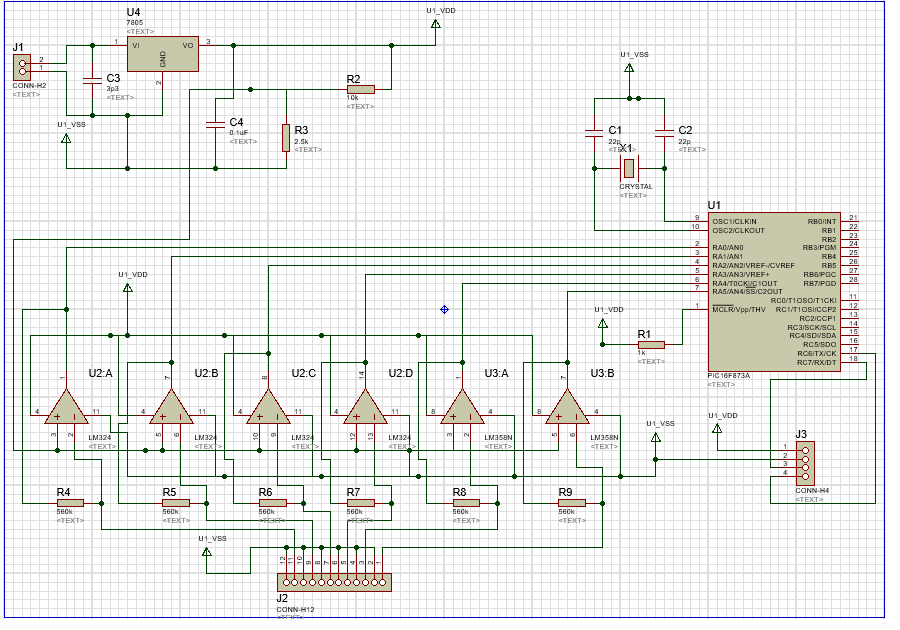
\includegraphics[width=1\textwidth]{./image/esquematico.png}
\caption{Esquemático}
\label{fig:esquematico}
\end{figure}

\newpage

\section{Documentación del Diseño PCB}

\begin{figure}[H]
\centering
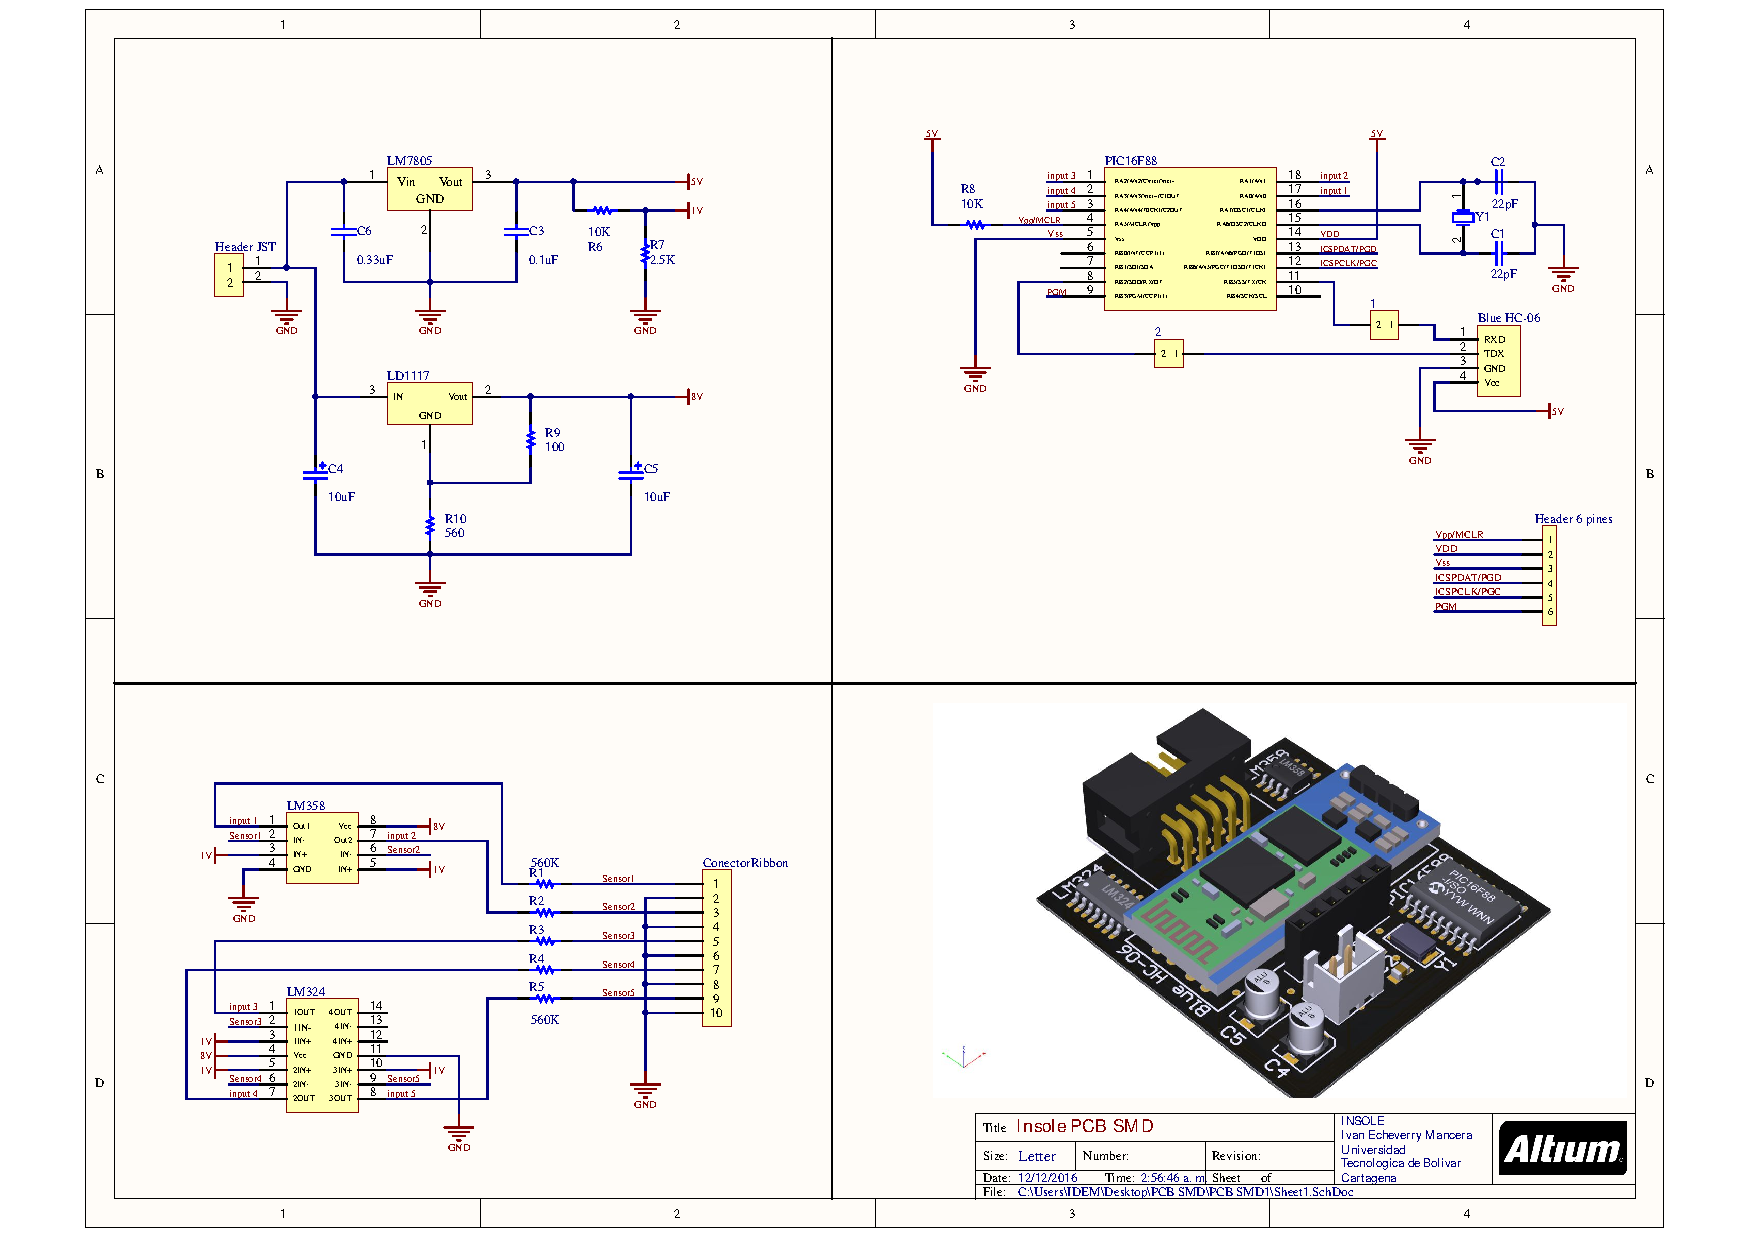
\includegraphics[width=1\textwidth]{./Documentos_PDF/DiagramaElectronico.pdf}
\caption{Diagrama Electrónico}
\label{fig:DiagramaElectronico}
\end{figure}

\begin{figure}[H]
\centering
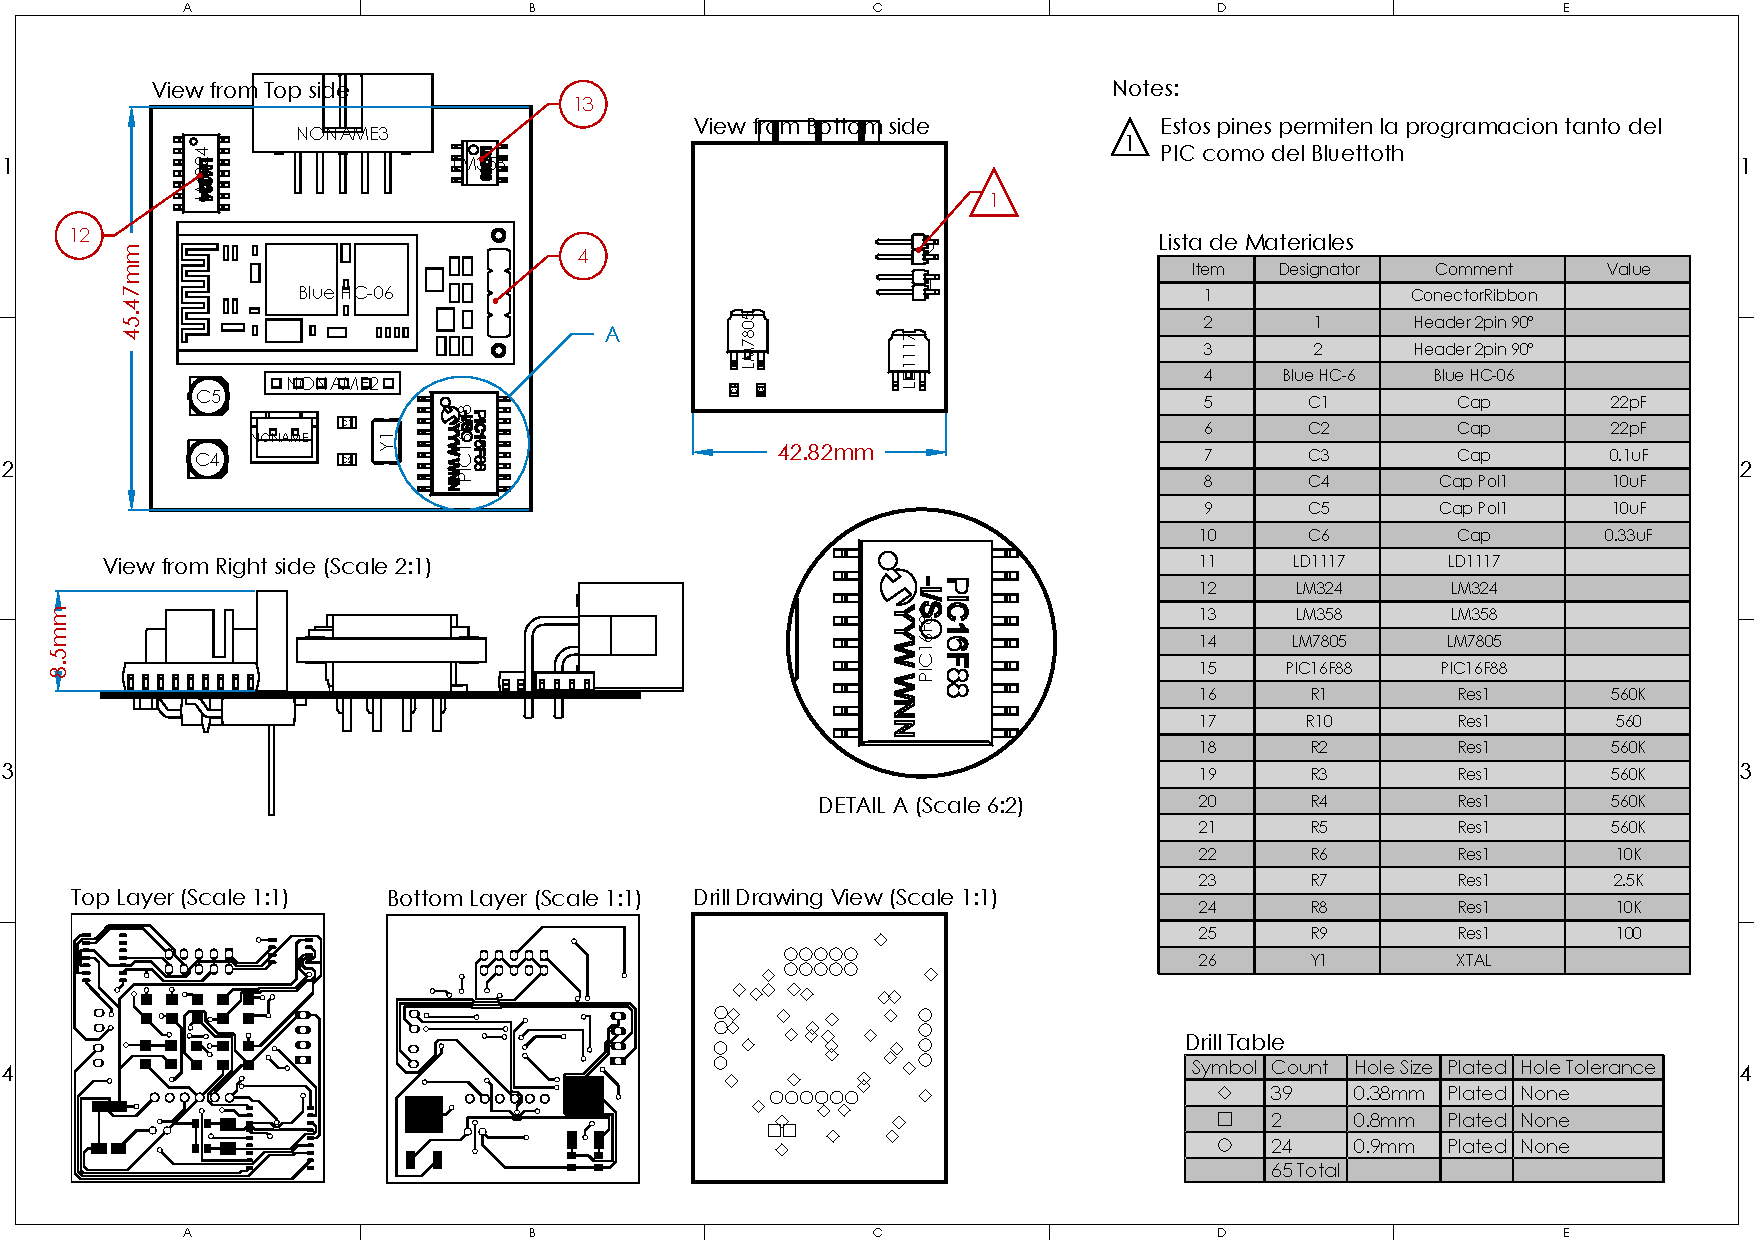
\includegraphics[width=1\textwidth]{./Documentos_PDF/Detalle_PCB.pdf}
\caption{Detalles del PCB}
\label{fig:PCB_Detalles}
\end{figure}

\begin{figure}[H]
\centering
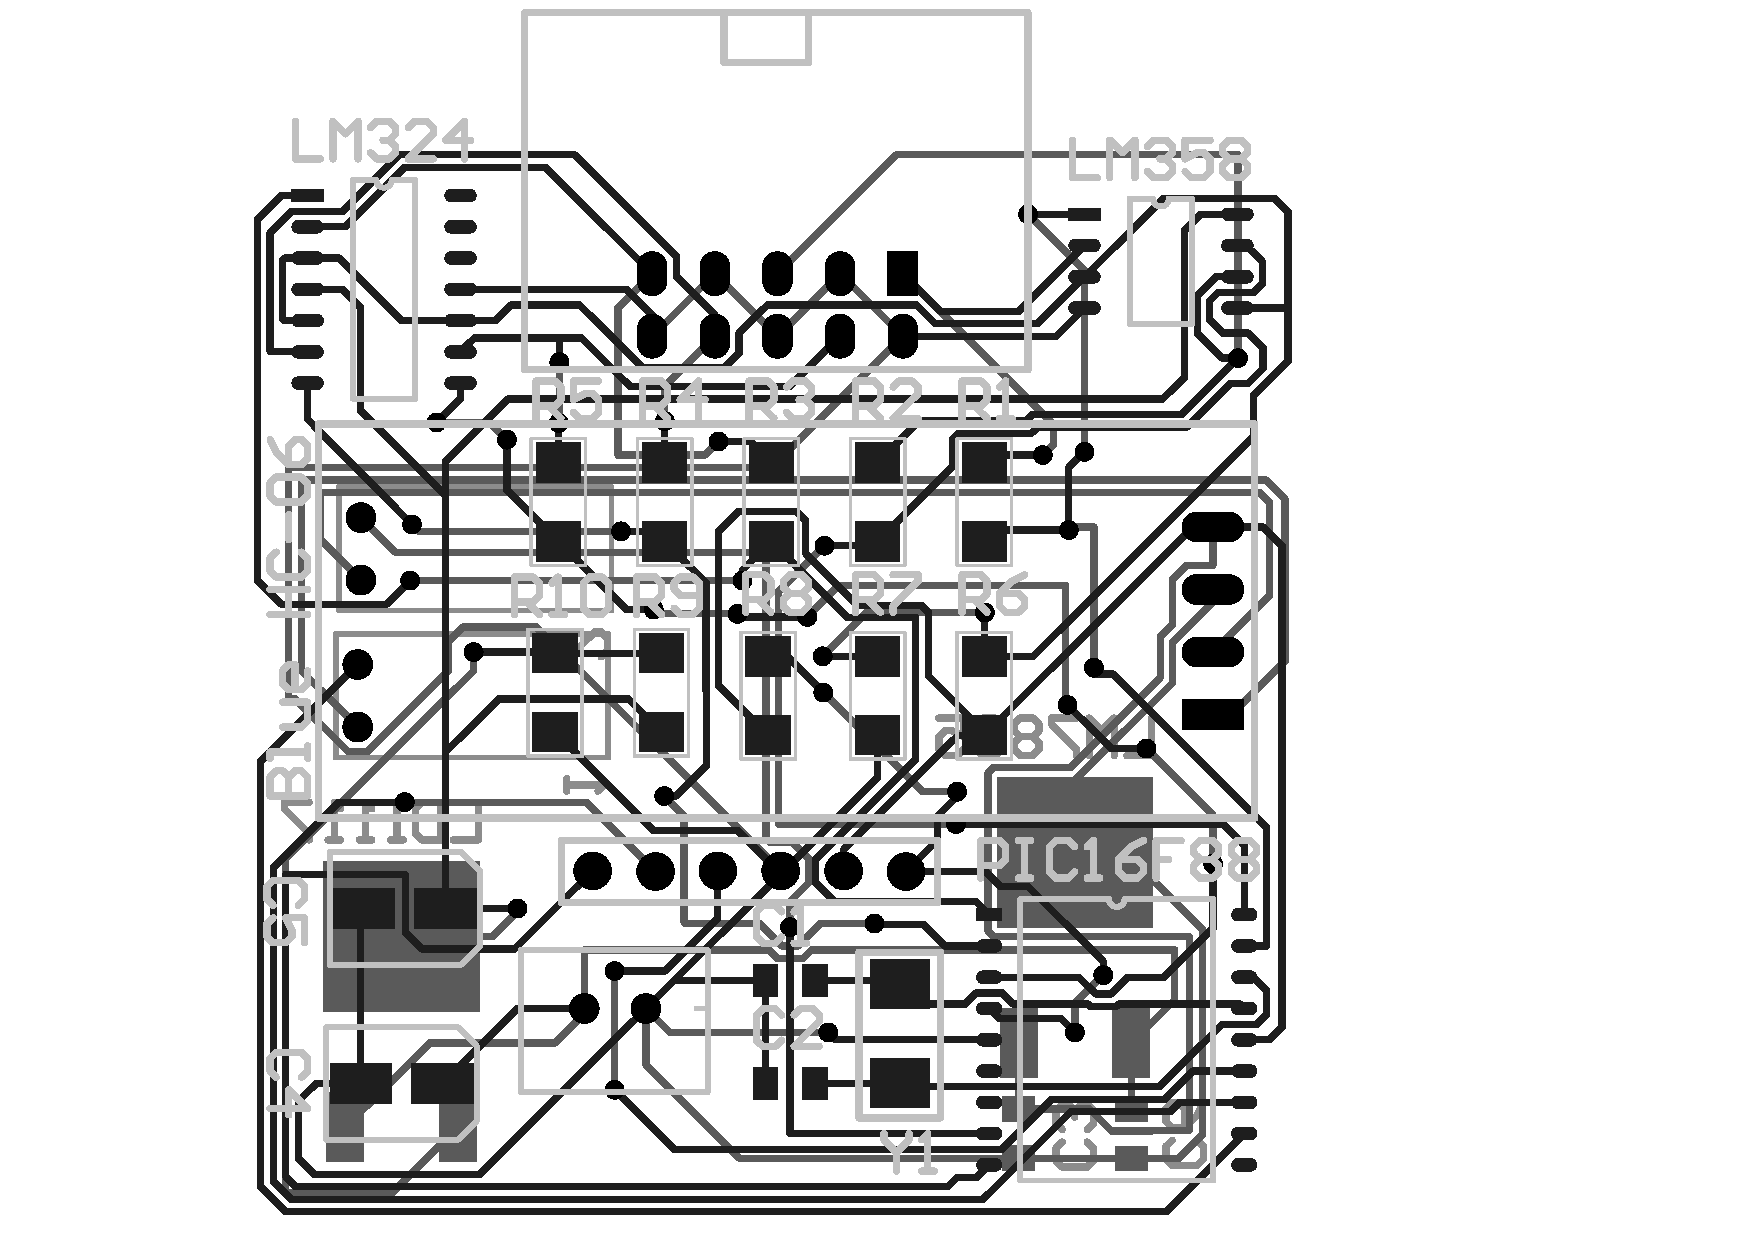
\includegraphics[width=1\textwidth]{./Documentos_PDF/Pistas_PCB.pdf}
\caption{Diseño de Pistas}
\label{fig:Pistas_PCB}
\end{figure}

\begin{figure}[H]
\centering
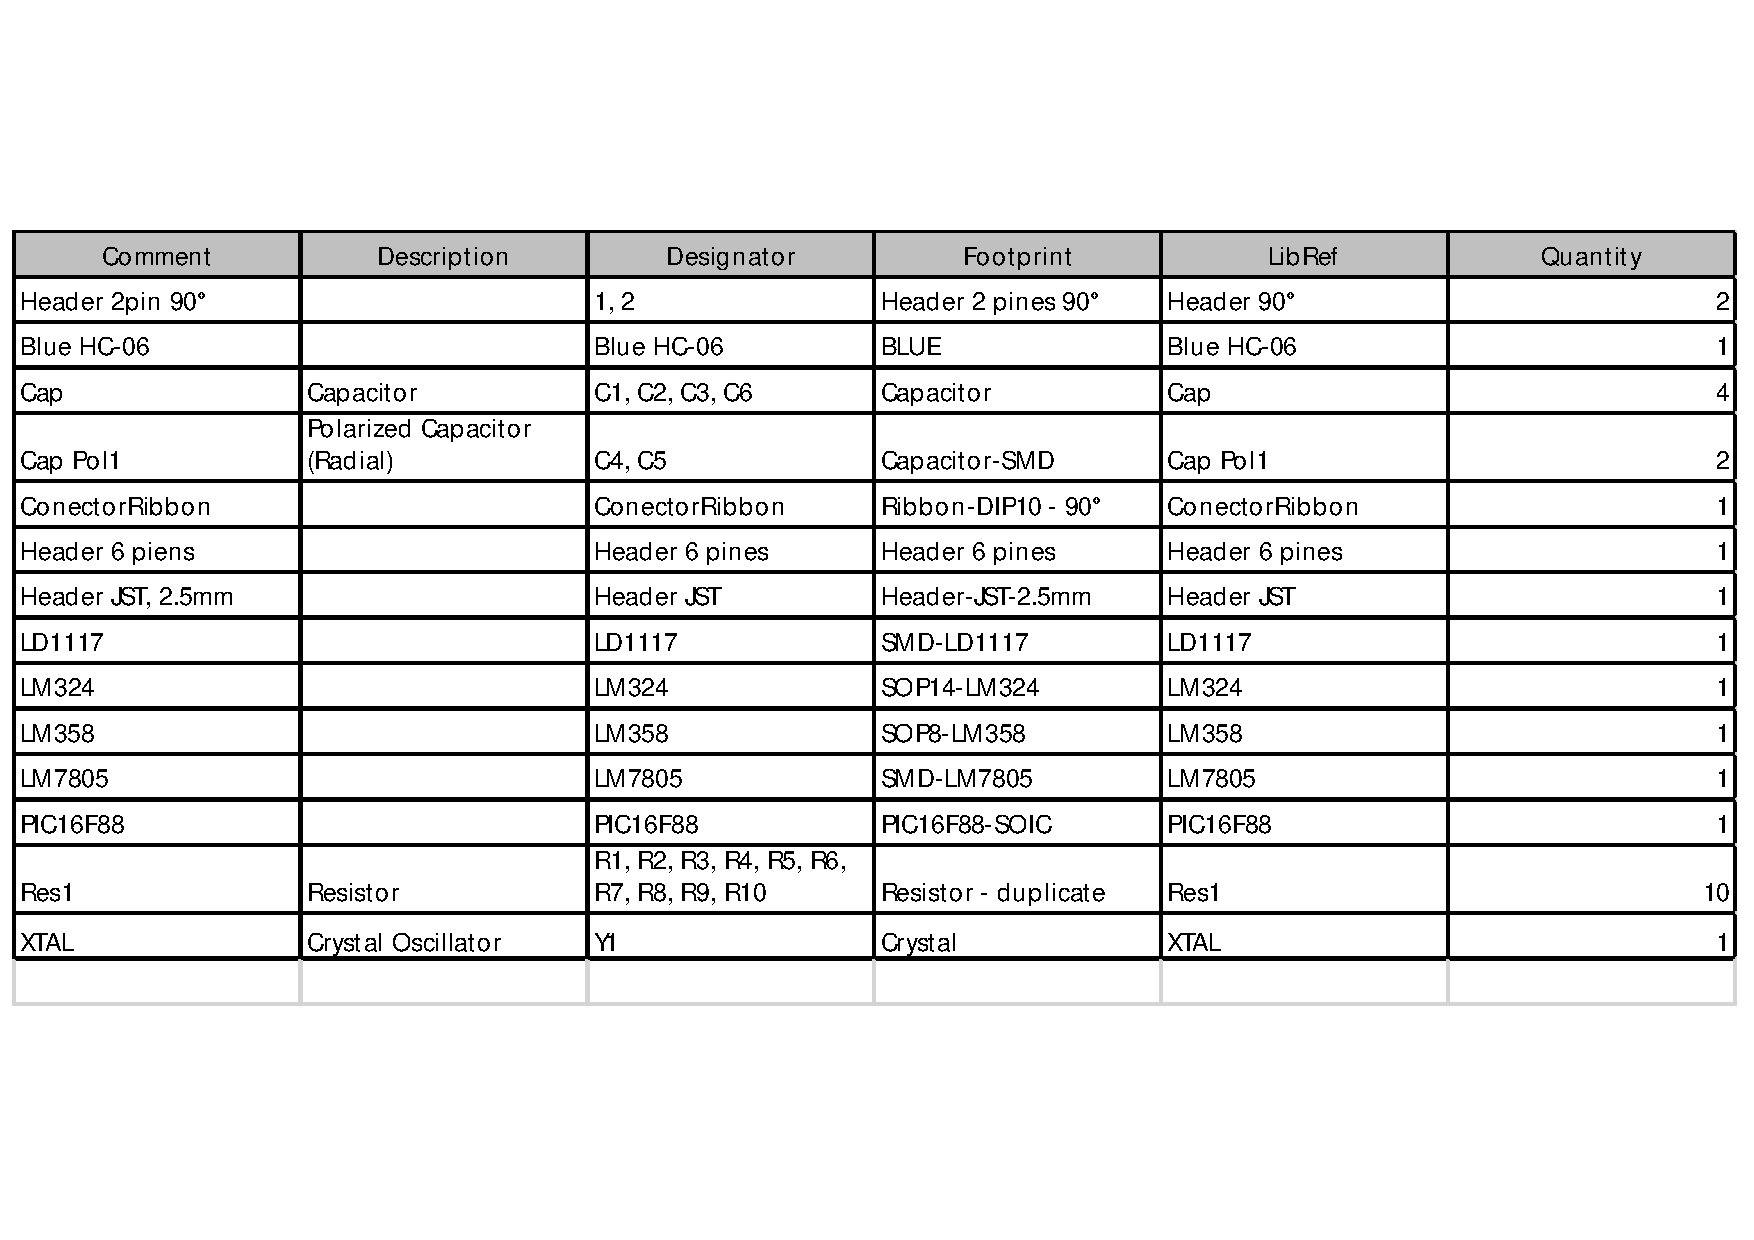
\includegraphics[width=1\textwidth]{./Documentos_PDF/Lista_Materiales.pdf}
\caption{Listas de Materiales PCB}
\label{fig:Lista_Materiales}
\end{figure}

\newpage

\section{Fotos del Sistema Insole}

\begin{figure}[H]
\centering
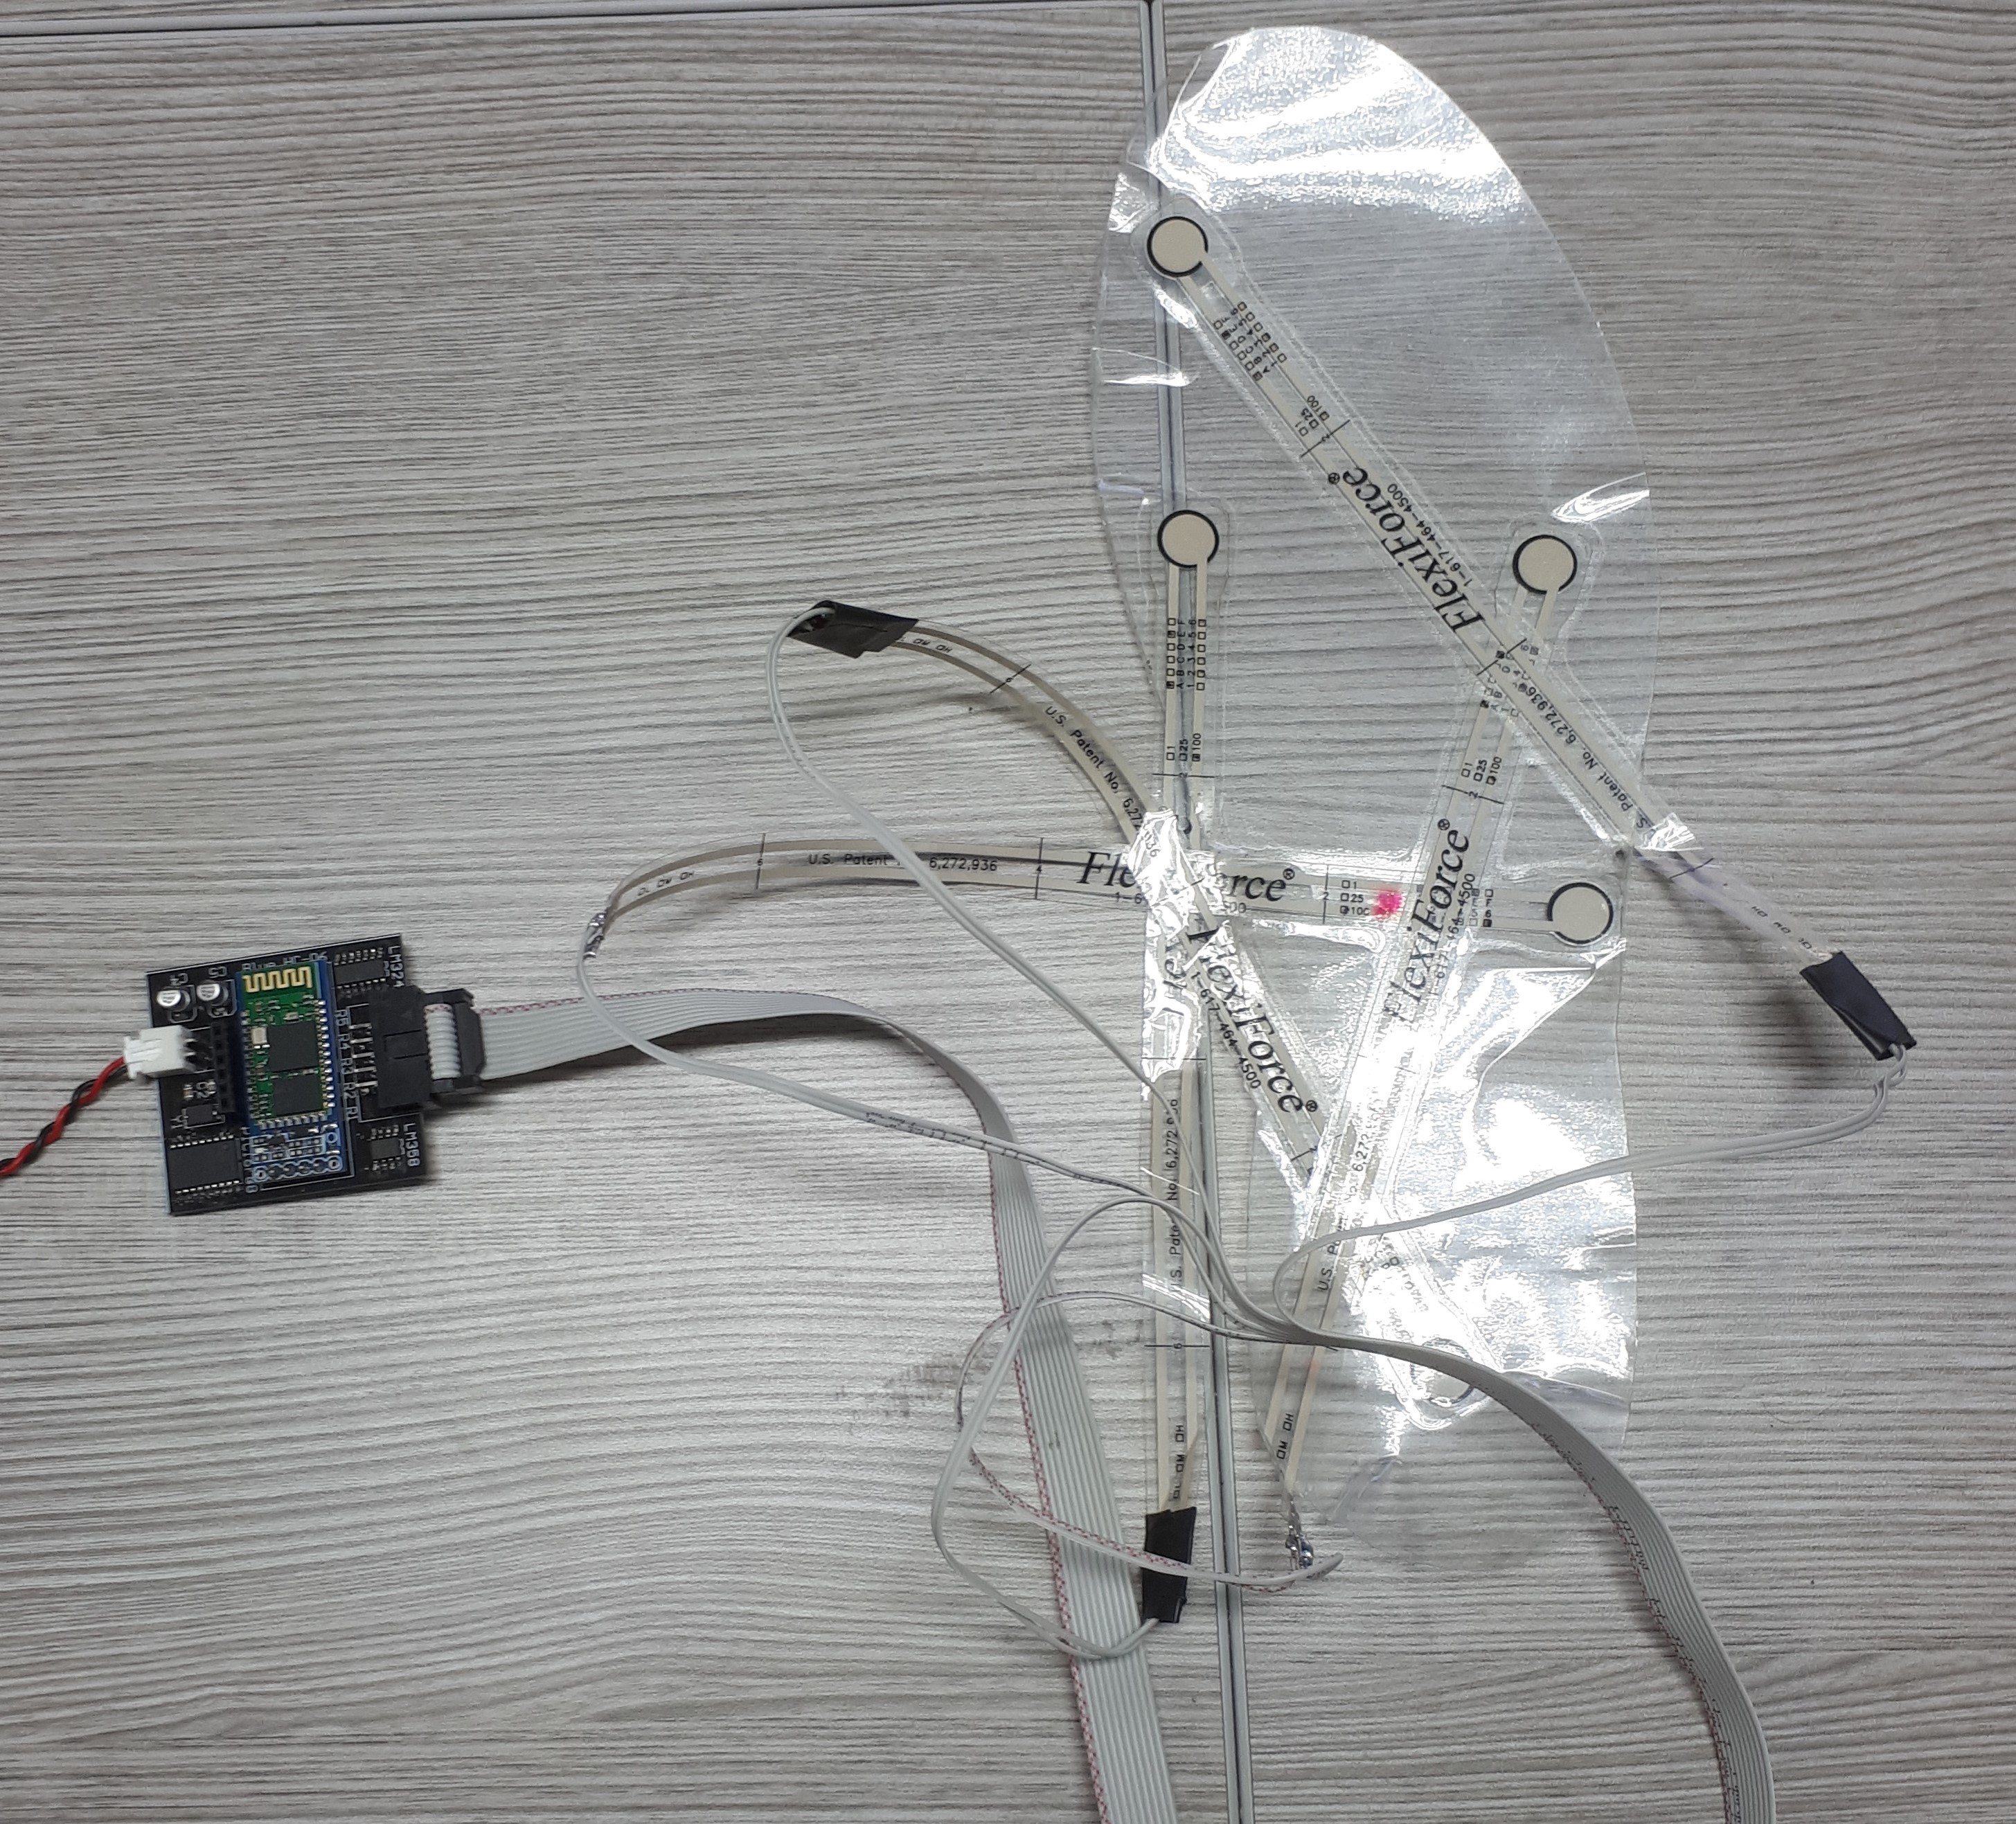
\includegraphics[width=1\textwidth]{./image/foto3.jpg}
\caption{Sistema de plantilla Insole Vista 1.}
\label{fig:plantillavista1}
\end{figure}

\begin{figure}[H]
\centering
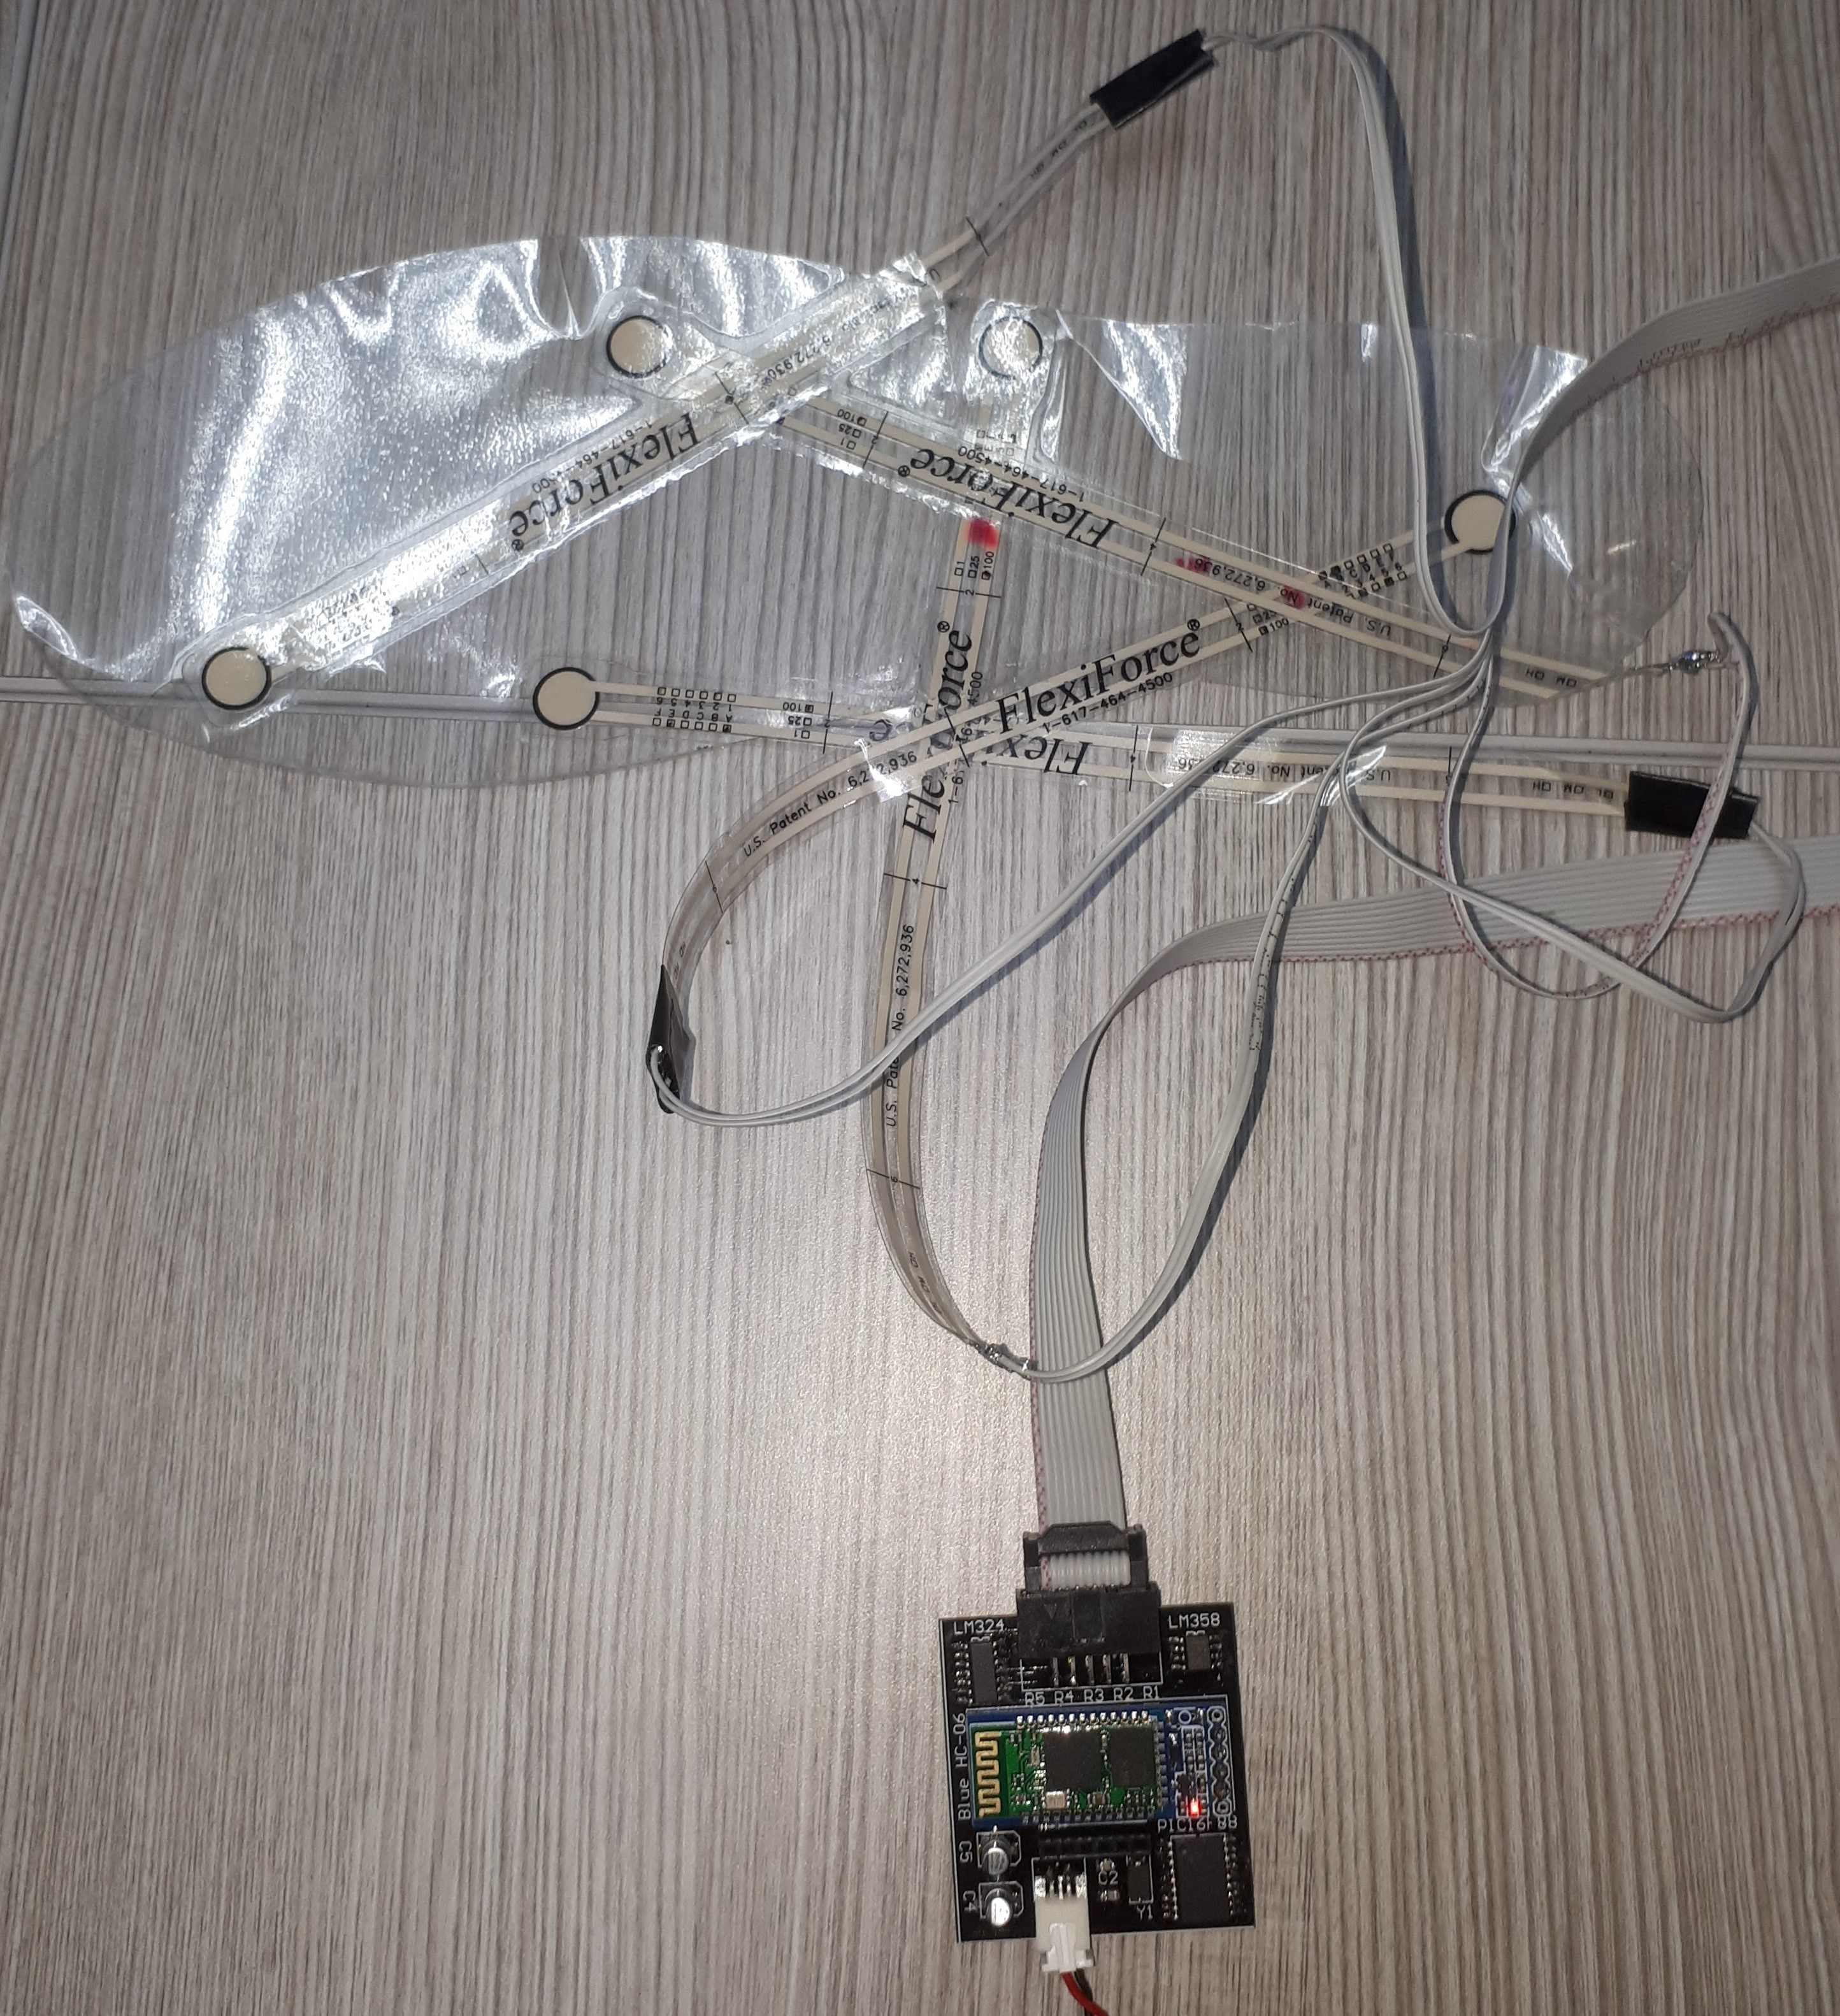
\includegraphics[width=1\textwidth]{./image/foto2.jpg}
\caption{Sistema de plantilla Insole Vista 2.}
\label{fig:plantillavista2}
\end{figure}

\begin{figure}[H]
\centering
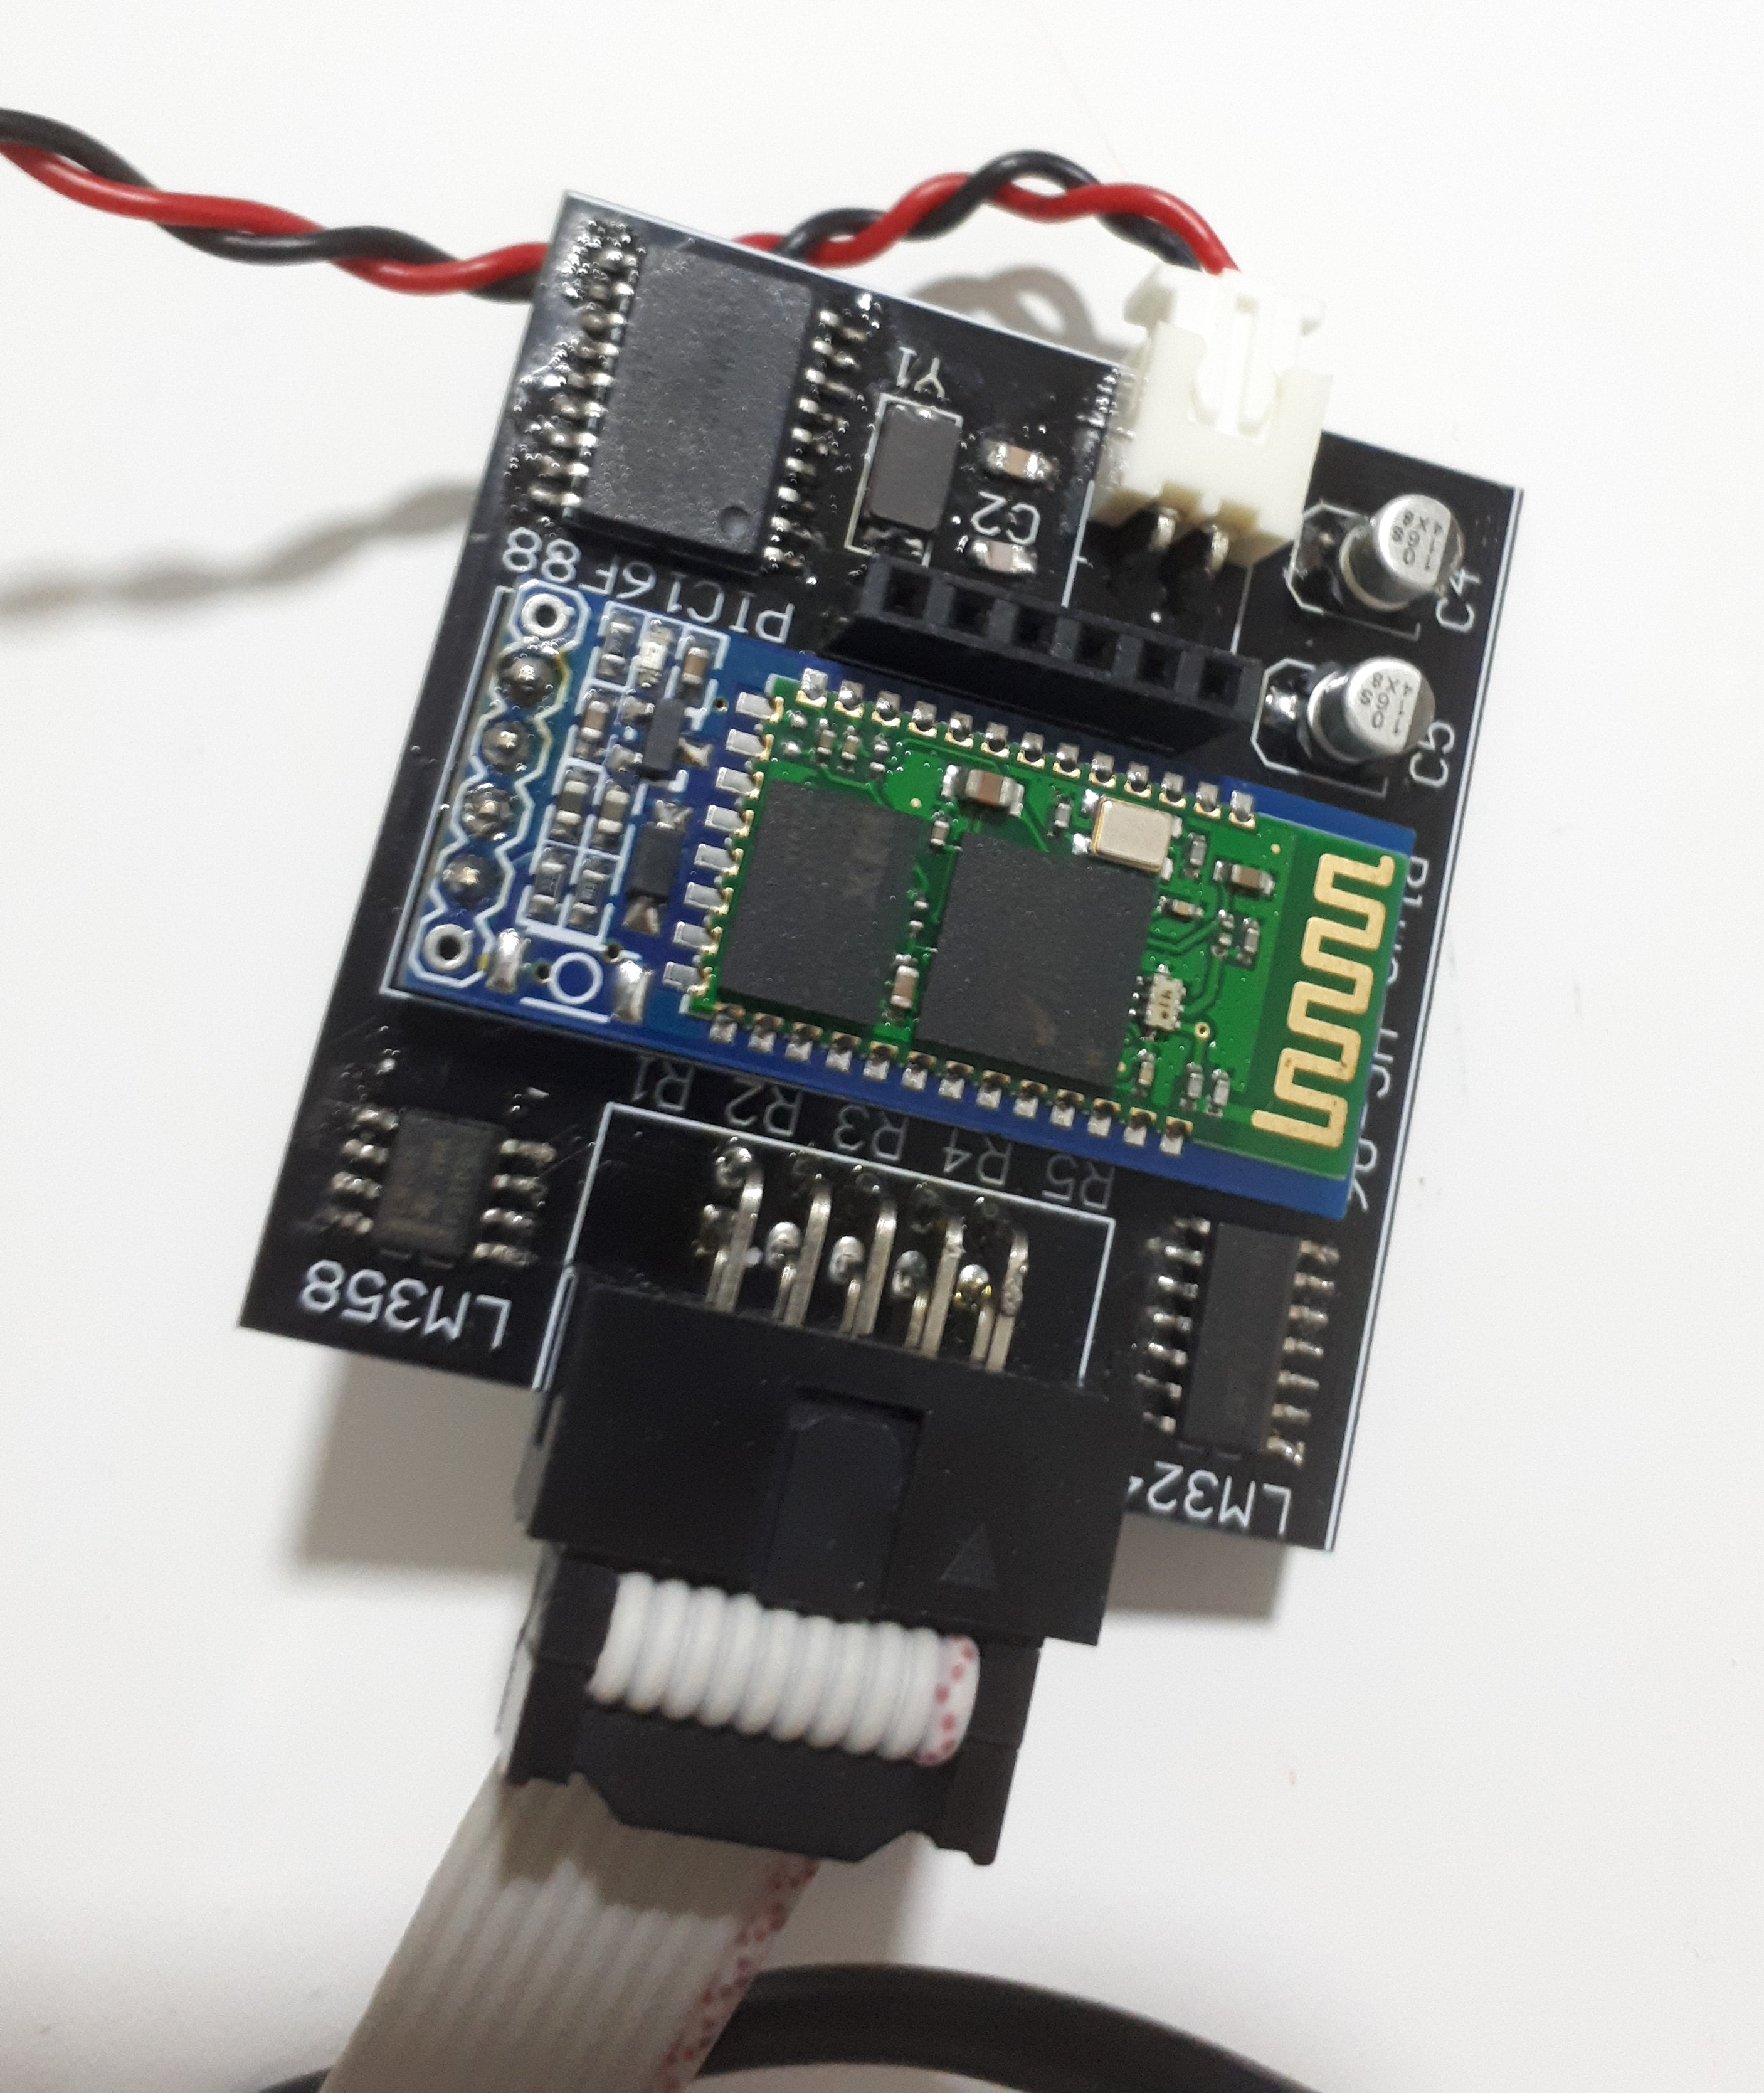
\includegraphics[width=1\textwidth]{./image/foto1.jpg}
\caption{Tarjeta electrónica captadora y transmisora de los datos.}
\label{fig:Tarjeta}
\end{figure}





	
%\par}
%abbrv
%unsrt

\pagestyle{empty}
\sloppy
\bibliographystyle{unsrt}
\bibliography{insole}

\end{document}
